\documentclass[11pt,oneside]{report}

\usepackage[T1]{fontenc}
\usepackage{lmodern}
\usepackage{microtype}
\usepackage[a4paper,margin=23mm,headheight=15pt]{geometry}
\usepackage{amsmath,amssymb,mathtools}
\usepackage{graphicx}
\usepackage{xcolor}
\usepackage{booktabs,longtable,tabularx,array,multirow,makecell}
\usepackage{float}
\usepackage{caption,subcaption}
\usepackage{pdflscape}
\usepackage{enumitem}
\usepackage{listings}
\usepackage{fancyhdr}
\usepackage{titlesec}
\usepackage{tikz}
\usetikzlibrary{arrows.meta,positioning,fit,shapes.geometric}
\usepackage[most]{tcolorbox}
\usepackage{xurl}
\usepackage{seqsplit}
\usepackage[numbers,sort&compress]{natbib}
\usepackage[hidelinks]{hyperref}
\usepackage[nameinlink,noabbrev]{cleveref}

\definecolor{CytoBlue}{HTML}{176B87}
\definecolor{CytoTeal}{HTML}{218C74}
\definecolor{CytoRed}{HTML}{C4455A}
\definecolor{CytoGold}{HTML}{D99A2B}
\definecolor{CytoPurple}{HTML}{735DA5}
\definecolor{CytoInk}{HTML}{24323D}
\definecolor{CytoPale}{HTML}{EEF4F7}

\hypersetup{
  colorlinks=true,
  linkcolor=CytoBlue,
  citecolor=CytoTeal,
  urlcolor=CytoPurple,
  pdftitle={CytoFair: Complete Project Record},
  pdfauthor={Snehasish Ghosh, Soham Mitra, Nibaran Das}
}

\titleformat{\chapter}[display]
  {\normalfont\huge\bfseries\color{CytoInk}}
  {\filleft\color{CytoBlue}\fontsize{42}{45}\selectfont\thechapter}
  {0.3ex}
  {\titlerule[1.2pt]\vspace{1ex}\filright}
\titleformat{\section}{\Large\bfseries\color{CytoInk}}{\thesection}{0.65em}{}
\titleformat{\subsection}{\large\bfseries\color{CytoBlue}}{\thesubsection}{0.65em}{}
\titleformat{\subsubsection}{\normalsize\bfseries\color{CytoTeal}}{\thesubsubsection}{0.65em}{}

\pagestyle{fancy}
\fancyhf{}
\fancyhead[L]{\small\color{CytoInk}CytoFair: Complete Project Record}
\fancyhead[R]{\small\color{CytoBlue}\nouppercase{\leftmark}}
\fancyfoot[C]{\color{CytoInk}\thepage}
\renewcommand{\headrulewidth}{0.4pt}
\setlength{\parindent}{0pt}
\setlength{\parskip}{0.55em}
\setcounter{tocdepth}{3}
\setcounter{secnumdepth}{3}

\newtcolorbox{keybox}[1]{
  enhanced,breakable,colback=CytoPale,colframe=CytoBlue,
  title={#1},fonttitle=\bfseries,boxrule=0.8pt,arc=1.5mm,
  left=2mm,right=2mm,top=1.5mm,bottom=1.5mm
}
\newtcolorbox{warningbox}[1]{
  enhanced,breakable,colback=CytoRed!5,colframe=CytoRed,
  title={#1},fonttitle=\bfseries,boxrule=0.8pt,arc=1.5mm,
  left=2mm,right=2mm,top=1.5mm,bottom=1.5mm
}
\newtcolorbox{decisionbox}[1]{
  enhanced,breakable,colback=CytoGold!8,colframe=CytoGold!85!black,
  title={#1},fonttitle=\bfseries,boxrule=0.8pt,arc=1.5mm,
  left=2mm,right=2mm,top=1.5mm,bottom=1.5mm
}
\newcommand{\protocol}[1]{\textsf{#1}}
\newcommand{\cytofair}{\textsc{CytoFair}}
\newcommand{\pass}{\textcolor{CytoTeal}{\textbf{PASS}}}
\newcommand{\fail}{\textcolor{CytoRed}{\textbf{FAIL}}}
\newcommand{\pending}{\textcolor{CytoGold!80!black}{\textbf{PENDING}}}
\newcommand{\meanpm}[2]{#1\,$\pm$\,#2}
\newcommand{\artifact}[1]{\path{#1}}
\graphicspath{{assets/}}

\lstdefinestyle{cyto}{
  basicstyle=\ttfamily\small,
  keywordstyle=\color{CytoBlue}\bfseries,
  commentstyle=\color{CytoTeal},
  stringstyle=\color{CytoPurple},
  backgroundcolor=\color{CytoPale},
  frame=single,rulecolor=\color{CytoBlue!45},
  breaklines=true,showstringspaces=false,
  numbers=left,numberstyle=\tiny\color{CytoInk!55},
  xleftmargin=1.7em,framexleftmargin=1.4em
}

\begin{document}

\begin{titlepage}
\centering
\vspace*{1.1cm}
{\color{CytoBlue}\rule{\textwidth}{2.2pt}}\\[1.1cm]
{\Huge\bfseries\color{CytoInk} Do We Train on Test Cells?\\[0.35cm]}
{\LARGE\color{CytoBlue} The Complete CytoFair Project Record\\[0.5cm]}
{\Large Motivation, provenance recovery, leakage measurement, models, statistics,\\
execution history, failures, verification, and reusable artifacts}\par
\vspace{1.25cm}
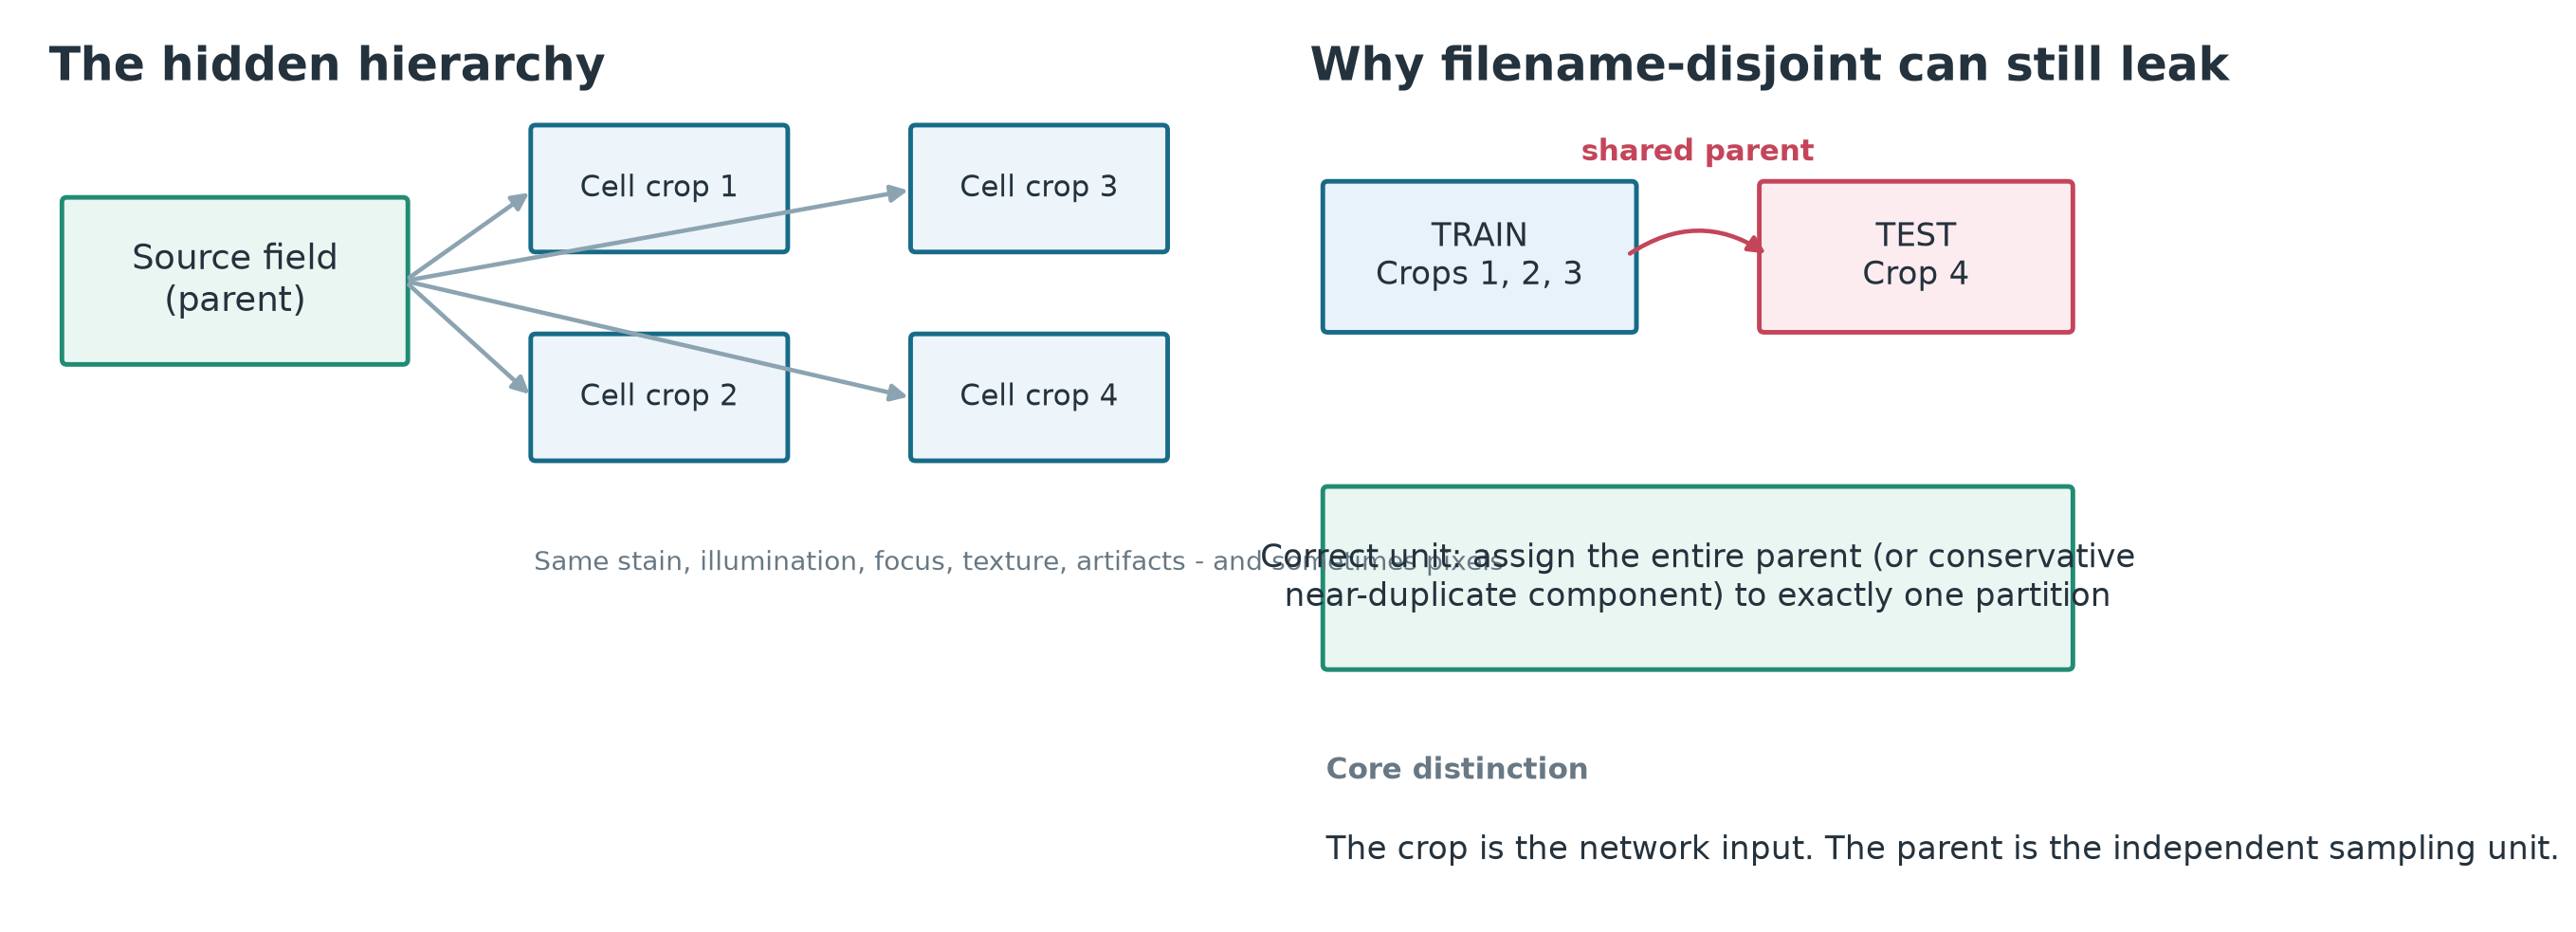
\includegraphics[width=0.92\textwidth]{hierarchy_and_leakage.png}
\vfill
{\Large\bfseries Snehasish Ghosh\textsuperscript{1}, Soham Mitra\textsuperscript{2}, Nibaran Das\textsuperscript{2}}\\[0.35cm]
{\normalsize
\textsuperscript{1}Indian Institute of Science, Bengaluru, India\\
\href{mailto:snehasishg@iisc.ac.in}{snehasishg@iisc.ac.in}\\[0.2cm]
\textsuperscript{2}Department of Computer Science and Engineering, Jadavpur University, Kolkata, India\\
Soham Mitra: \textit{[email placeholder]} \quad Nibaran Das: \textit{[email placeholder]}}
\vfill
{\large Frozen evidence through 7 September 2026\\
Comprehensive report compiled 13 September 2026 (Asia/Kolkata)}\\[0.5cm]
{\color{CytoBlue}\rule{\textwidth}{2.2pt}}
\end{titlepage}

\pagenumbering{roman}
\chapter*{Document status and scope}
\addcontentsline{toc}{chapter}{Document status and scope}

This is the long-form technical record of the \cytofair{} project. It is intentionally broader than the six-page conference paper. It explains why the project was started, how every analysis was designed, how the code represents the data, what was measured, what worked, what failed, what was changed during execution, what remains unverified, and what artifacts can be reused. The report is written from the repository state and frozen result files; it does not add a new experiment.

\begin{keybox}{Evidence boundary}
The quantitative claims in this document come from committed CSV, JSON, Parquet, source, and report artifacts in the repository. The experiment inventory contains 120 SIPaKMeD classification runs, 30 parent-identity probe runs, and 175 Cx22 segmentation runs: 325 completed neural-network runs in total. Structural analyses are additional deterministic or Monte Carlo computations, not neural runs. No post-hoc classifier confusion matrix or qualitative model prediction is invented, because the frozen classifier JSON files retain aggregate metrics and epoch histories but not per-sample predictions or checkpoints.
\end{keybox}

\begin{warningbox}{How to interpret ``leakage'' in this report}
Structural non-independence, literal pixel overlap, and a learnable parent fingerprint are demonstrated. These facts establish that a shortcut is available. They do \emph{not} prove that every cervical-classification model causally uses that shortcut, and the multiplicity-corrected classifier contrasts do not establish a universal accuracy-inflation effect. This distinction is maintained throughout the report.
\end{warningbox}

\begin{abstract}
Cervical-cell datasets are frequently released as crops, even when several crops came from one microscopic field or source image. A random crop split can therefore place sibling crops in both training and test sets, making file-level disjointness look like biological or acquisition-level independence. CytoFair recovers the hidden crop-to-parent hierarchy, validates it with fail-closed checks, measures structural and literal overlap, constructs parent- and component-disjoint splits, probes whether source identity remains learnable after transformations, and re-scores classification and segmentation models under matched protocols. The audit recovered all 4,049 SIPaKMeD crops, 1,320 Cx22 regions, 11,534 CRIC cells, and 917 Herlev cells. Under random splitting, 92.62\% of SIPaKMeD test crops, 85.23\% of Cx22 test regions, and 99.97\% of CRIC test cells had a parent in training, whereas Herlev correctly remained at zero. More than half of SIPaKMeD test crops shared literal source pixels with a training crop. A 424-way parent probe reached 25.73\% accuracy against 0.2358\% chance. All six SIPaKMeD classifier P1--P2 point estimates and all seven Cx22 segmentation estimates were positive, but no confirmatory contrast survived its preregistered Benjamini--Hochberg family. The project therefore supports a strong benchmark-construction conclusion---evaluate at the independent parent unit---while retaining a narrower and appropriately uncertain model-performance conclusion.
\end{abstract}

\tableofcontents
\listoffigures
\listoftables
\clearpage
\pagenumbering{arabic}

\chapter{Executive overview}

\section{The entire project in one page}

The initial problem was simple to state: \emph{when a benchmark calls every image file an independent example, is that file really the unit that was independently sampled?} In cervical cytology, the answer can be no. One microscope field can emit several cell crops. If those crops are split independently, their source field can appear on both sides of evaluation.

The project followed a staged answer:
\begin{enumerate}[leftmargin=2em]
  \item define the independent parent unit for four public datasets;
  \item recover exact crop-to-parent mappings, using independent recovery branches where the release permits them;
  \item refuse downstream analysis unless agreement, geometry, counts, and uniqueness pass;
  \item calculate how often random crop splitting separates siblings;
  \item detect literal pixel overlap and conservative cross-parent near-duplicate components;
  \item create four fixed protocols that isolate independence from training-set size;
  \item ask whether parent identity is visually learnable after removing candidate cues;
  \item re-run multiple classifier and segmentation families over five fixed seeds;
  \item use paired inference, effect sizes, bootstrap intervals, and declared BH families;
  \item preserve failed attempts and execution amendments rather than erasing them.
\end{enumerate}

\begin{figure}[H]
\centering
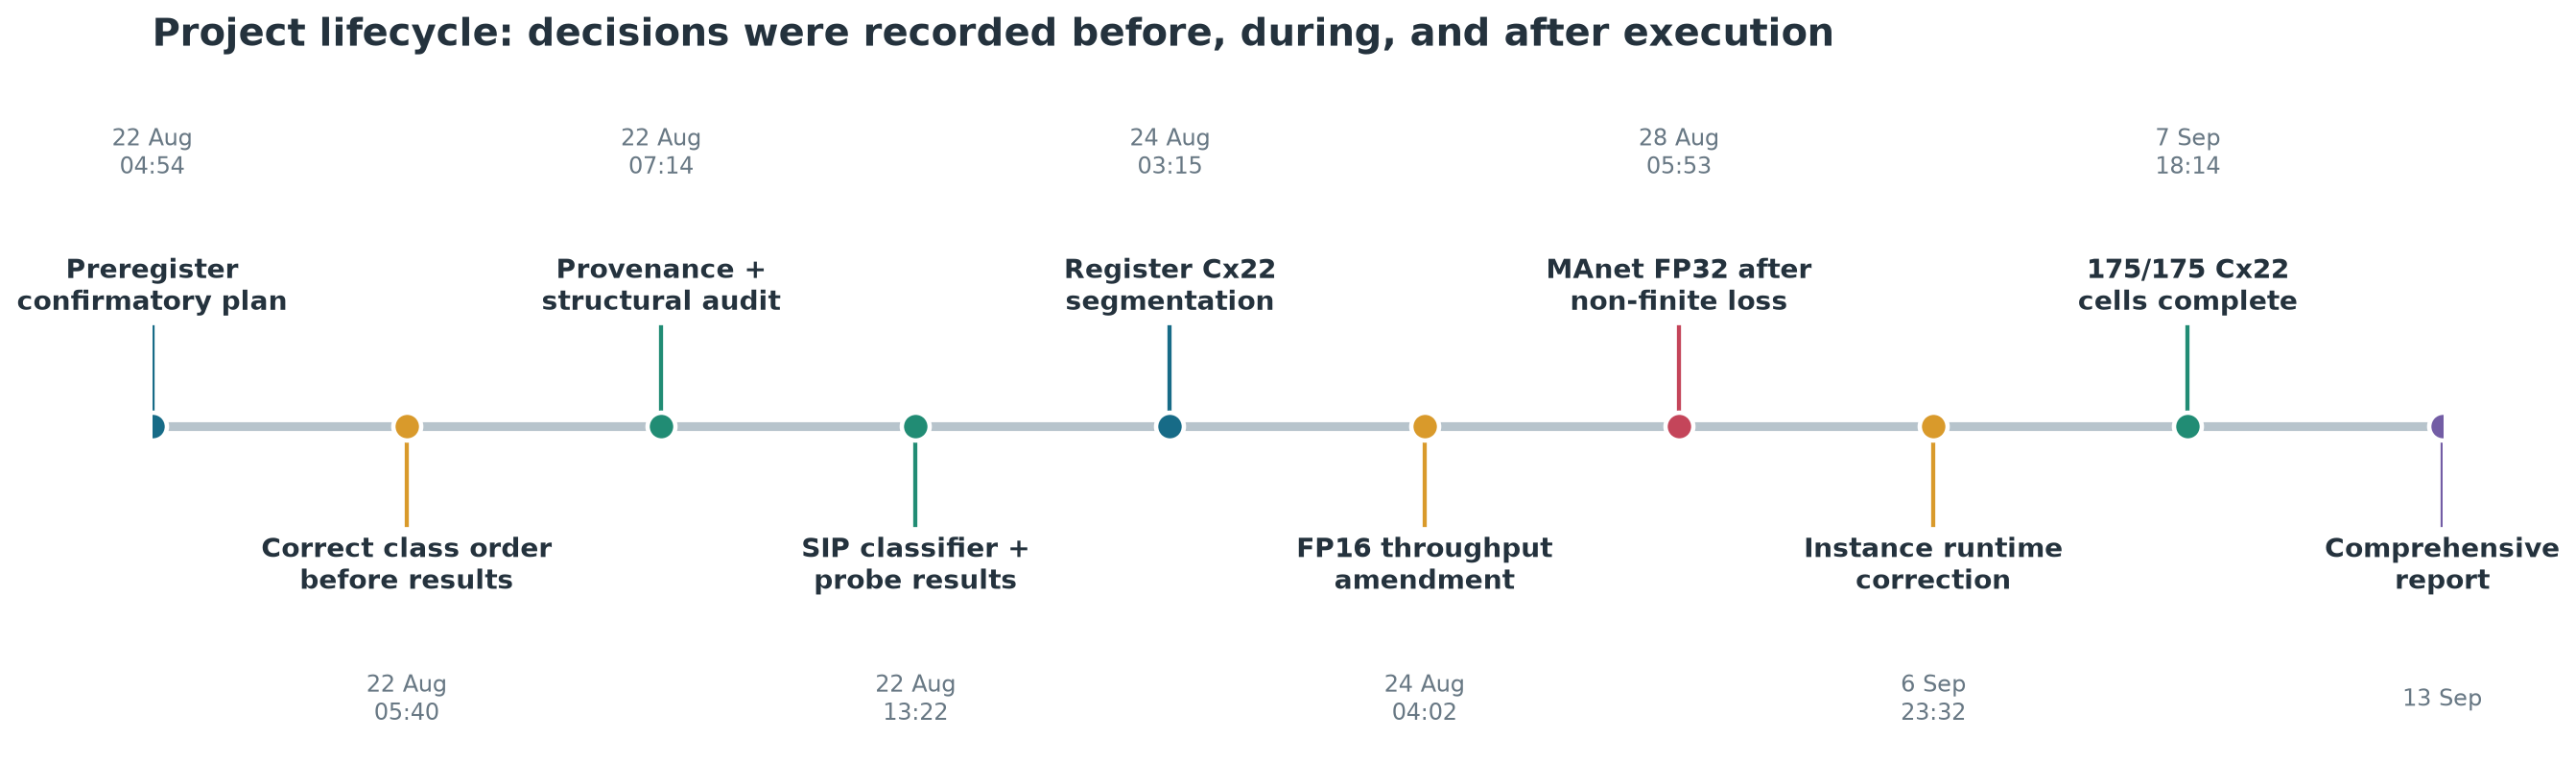
\includegraphics[width=\textwidth]{lifecycle_timeline.png}
\caption{The project lifecycle. Blue events register decisions, green events record completed evidence, gold events document execution-driven amendments, red records a numerical failure, and purple marks this report.}
\label{fig:lifecycle}
\end{figure}

\section{Headline findings, without spin}

\begin{longtable}{p{0.22\textwidth}p{0.19\textwidth}p{0.51\textwidth}}
\caption{Headline conclusions and their correct strength.}\label{tab:headline}\\
\toprule
Question & Answer & Evidence and boundary \\
\midrule
\endfirsthead
\toprule
Question & Answer & Evidence and boundary \\
\midrule
\endhead
\bottomrule
\endfoot
Can provenance be recovered? & Yes & SIPaKMeD branches agree on 4,049/4,049 crops; all boxes are contained; all dataset and class totals match. \\
Does random crop splitting share parents? & Yes & Mean P1 test-parent overlap is 92.62\% on SIPaKMeD, 85.23\% on Cx22, and 99.97\% on CRIC. \\
Does the negative control remain negative? & Yes & Herlev has one released cell per parent and returns exactly 0.00\% structural leakage for all seeds. \\
Are literal pixels shared? & Yes, in SIPaKMeD P1 & 52.62\% of test crops share at least one source pixel with a training crop; P2/P3 return zero. \\
Is source identity learnable? & Yes & A 424-way ResNet-18 reaches 25.73\% versus 0.2358\% chance; shuffled labels return 0.17\% and cover chance. \\
Is P1 accuracy universally inflated? & Not established & All six SIPaKMeD and all seven Cx22 P1--P2 means are positive, but no contrast survives BH correction. \\
Does stronger grouping always lower score? & No & SIPaKMeD's registered P3 $\leq$ P2 $\leq$ P1 model ordering fails for four of six architectures. The failure is retained. \\
Is Cx22's official split defective? & No such claim & The authors' Multi-Train/Multi-Test parent sets are disjoint. The pooled stress test asks what happens under a different downstream reuse pattern. \\
Is the release fully ready? & Not yet & The clean-clone/virgin-host evidence, lab-paper crosswalk, and independent Figure-1 reader gate remain pending. \\
\end{longtable}

\chapter{Motivation and problem formulation}

\section{Why cervical cytology makes independence important}

Cervical cancer caused an estimated 660,000 new cases and 350,000 deaths worldwide in 2022~\cite{who2025hpv}. Cytology screening is a high-volume recognition problem: a small number of clinically important abnormal cells must be found among many plausible normal cells. Automation is attractive because it can help direct expert attention, but only if reported generalization represents genuinely unseen biological or acquisition units.

Modern cervical-cell classifiers report very high crop-level scores. DeepPap reported 98.3\% on Herlev~\cite{zhang2017deeppap}; DeepCervix reported 99.14\% on SIPaKMeD~\cite{rahaman2021deepcervix}; and a knowledge-distillation system reported 98.52\% on SIPaKMeD~\cite{gao2022knowledge}. These achievements motivated a basic audit question that is logically prior to choosing a stronger network: \emph{what population unit does the test set represent?}

\section{Observation, parent, and evaluation unit}

Let $x_i$ be a released image observation and let $g(x_i)=p_j$ map it to the acquisition unit that generated it. In this project:
\begin{itemize}
  \item $x_i$ is a SIPaKMeD cell crop and $p_j$ is a cluster field;
  \item $x_i$ is a Cx22 generated region and $p_j$ is a CCEDD source image;
  \item $x_i$ is a CRIC annotated cell and $p_j$ is its source smear image;
  \item $x_i$ is a Herlev single-cell image and is also its own parent.
\end{itemize}

The crucial idea is that the \emph{model input} and the \emph{independent sampling unit} need not be the same object. A network consumes $x_i$, but the statistical independence boundary may be $p_j$.

\begin{figure}[H]
\centering
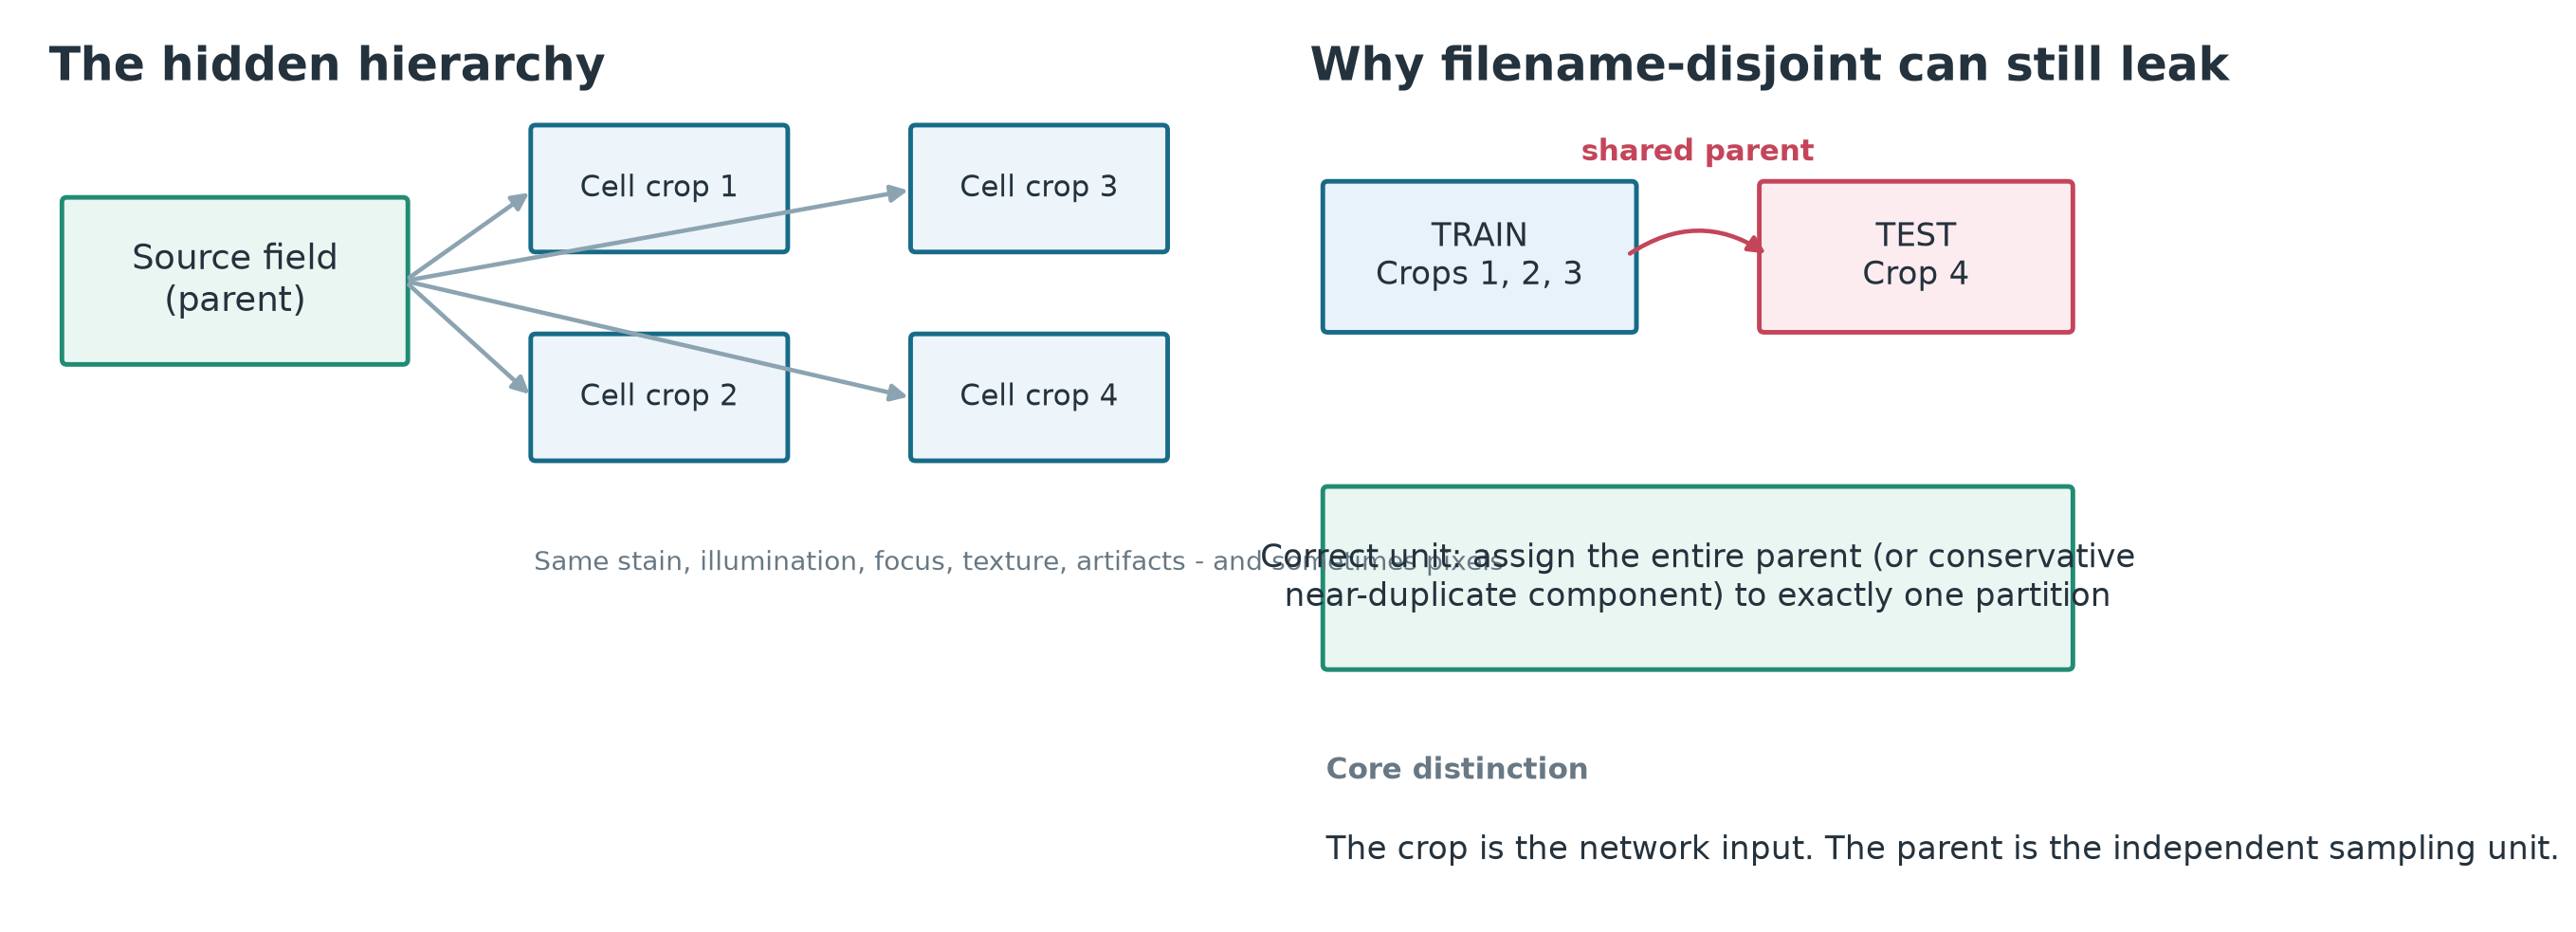
\includegraphics[width=\textwidth]{hierarchy_and_leakage.png}
\caption{The hidden hierarchy and the central failure mode. Several file-disjoint crops can share a parent field, source-specific nuisance factors, or literal source pixels.}
\label{fig:hierarchy}
\end{figure}

\section{Three different claims that must not be conflated}

\begin{keybox}{Claim 1: structural non-independence}
Some parents contribute observations to both train and test. This can be established exactly from provenance and split assignments. It requires no model.
\end{keybox}

\begin{keybox}{Claim 2: shortcut availability}
A model can identify the source parent from held-out sibling crops at greater-than-chance accuracy. This shows that parent information survives in the released input. It does not yet show that a disease or morphology classifier uses it.
\end{keybox}

\begin{keybox}{Claim 3: downstream score inflation}
A crop-level protocol produces a larger score than a parent-disjoint protocol under matched models, seeds, and sample sizes. This is an empirical paired comparison. It needs uncertainty, multiplicity correction, and careful interpretation.
\end{keybox}

The project obtains strong evidence for Claims 1 and 2. For Claim 3, point estimates are directionally consistent across every tested architecture, but the confirmatory families do not cross the multiplicity-adjusted threshold. The report therefore never upgrades ``available shortcut'' into ``proven universal causal inflation.''

\section{Relationship to leakage and duplicate audits}

Duplicate-aware evaluation has been studied in general vision: ciFAIR removed near-duplicate CIFAR test counterparts~\cite{barz2020cifair}; license-plate work re-evaluated models under duplicate-free splits~\cite{laroca2023lpr}; and medical-image re-identification demonstrated that patient identity can be highly learnable~\cite{packhauser2022reidentification}. Kapoor and Narayanan place these problems in a broader taxonomy of data leakage and reproducibility failures~\cite{kapoor2023leakage}. CytoFair's distinctive concern is an exact cervical-cytology source hierarchy: sibling crops can be non-independent without being duplicate files.

\chapter{Preregistration and analysis governance}

\section{Why the plan was committed first}

The original preregistration was committed at 04:54:10 IST on 22 August 2026 (commit \artifact{67e8ded}). The first result commit was recorded at 13:22:42 IST that day (commit \artifact{1c2da7f}). The plan therefore predates the committed results. This matters because a five-seed matrix contains many possible comparisons; fixing endpoints, seeds, exclusions, and multiplicity families before seeing scores reduces analyst degrees of freedom.

The fixed confirmatory seeds were $17,29,43,71,101$. Five additional robustness seeds were named but were not needed for the reported confirmatory summaries and were not substituted for any unfavorable seed. Every protocol-architecture cell had to contain at least five valid paired runs before inferential output could be emitted.

\section{Registered endpoints}

The structural endpoints were (i) fraction of parents straddling train and test and (ii) fraction of test observations whose parent appears in training. The mechanistic endpoint was 424-way parent-identification accuracy. The SIPaKMeD model endpoint was test accuracy; macro-F1 and balanced accuracy were concordance metrics. For Cx22 semantic segmentation, the primary endpoint was mean per-image cytoplasm/nucleus Dice. For Cx22 instance segmentation, the primary endpoint was per-image mean ground-truth-instance Dice after maximum-weight matching, with unmatched targets assigned zero.

\section{Amendments: what changed and why}

\begin{longtable}{p{0.10\textwidth}p{0.16\textwidth}p{0.26\textwidth}p{0.34\textwidth}}
\caption{Registered amendments and their evidential status.}\label{tab:amendments}\\
\toprule
Date & Amendment & Trigger & Why it did not select a favorable result \\
\midrule
\endfirsthead
\toprule
Date & Amendment & Trigger & Why it did not select a favorable result \\
\midrule
\endhead
\bottomrule
\endfoot
22 Aug & SIPaKMeD class order & The integrity gate exposed a transcription swap between Metaplastic and Dyskeratotic. & Corrected before any SIPaKMeD result; numeric target vector 126/108/238/271/223 did not change. \\
24 Aug & Cx22 segmentation extension & Structural Cx22 results motivated a separately scoped model rescore. & Registered before any Cx22 model was trained; official split retained as descriptive control. \\
24 Aug & FP16 execution & Full FP32 preflight left three A6000s under-used and made one U-Net epoch exceed 4.5 minutes. & Changed numerical execution before an epoch emitted a result; models, splits, seeds, endpoints, and epoch count stayed fixed. \\
28 Aug & MAnet in FP32 & The first MAnet P1 seed-17 attempts produced non-finite losses at epochs 23 and 24. & No completed MAnet result existed. All MAnet cells restarted from their fixed seeds rather than selecting a pre-divergence checkpoint. \\
28 Aug & Deterministic CUDA workspace & Startup warnings showed deterministic matrix multiplication required \artifact{CUBLAS_WORKSPACE_CONFIG=:4096:8}. & Frozen before a corrected MAnet or instance epoch existed; applied to all remaining cells. \\
6 Sep & Instance runtime correction & Evaluation every epoch, CPU mask matching, and frequent network checkpoint writes caused severe under-utilization. & The registered endpoint was final epoch. Intermediate test inference was removed, exact binary intersections moved to GPU, and recovery checkpoints became five-epoch; final computation stayed identical. \\
\end{longtable}

\begin{decisionbox}{A useful demotivation}
The project began with the possibility of a large, architecture-general accuracy correction. The statistics did not support that broad claim. Instead of hiding this, the project narrowed its claim: the benchmark hierarchy is demonstrably non-independent, the source signal is demonstrably learnable, and parent grouping removes the measured sharing. The size of downstream score inflation remains model- and task-dependent.
\end{decisionbox}

\chapter{Datasets and the hidden hierarchy}

\section{Overview}

\begin{table}[H]
\centering
\caption{Audited datasets and independent units.}
\label{tab:datasets}
\begin{tabularx}{\textwidth}{lrrrXX}
\toprule
Dataset & Observations & Parents & Mean/parent & Released task & Parent definition \\
\midrule
SIPaKMeD & 4,049 & 966 & 4.19 & 5-class classification & cluster field \\
Cx22 & 1,320 & 514 & 2.57 & semantic/instance segmentation & CCEDD source image \\
CRIC & 11,534 & 400 & 28.84 & cytology classification resource & source smear image \\
Herlev & 917 & 917 & 1.00 & 7-class single-cell classification & released cell image \\
\bottomrule
\end{tabularx}
\end{table}

\begin{figure}[H]
\centering
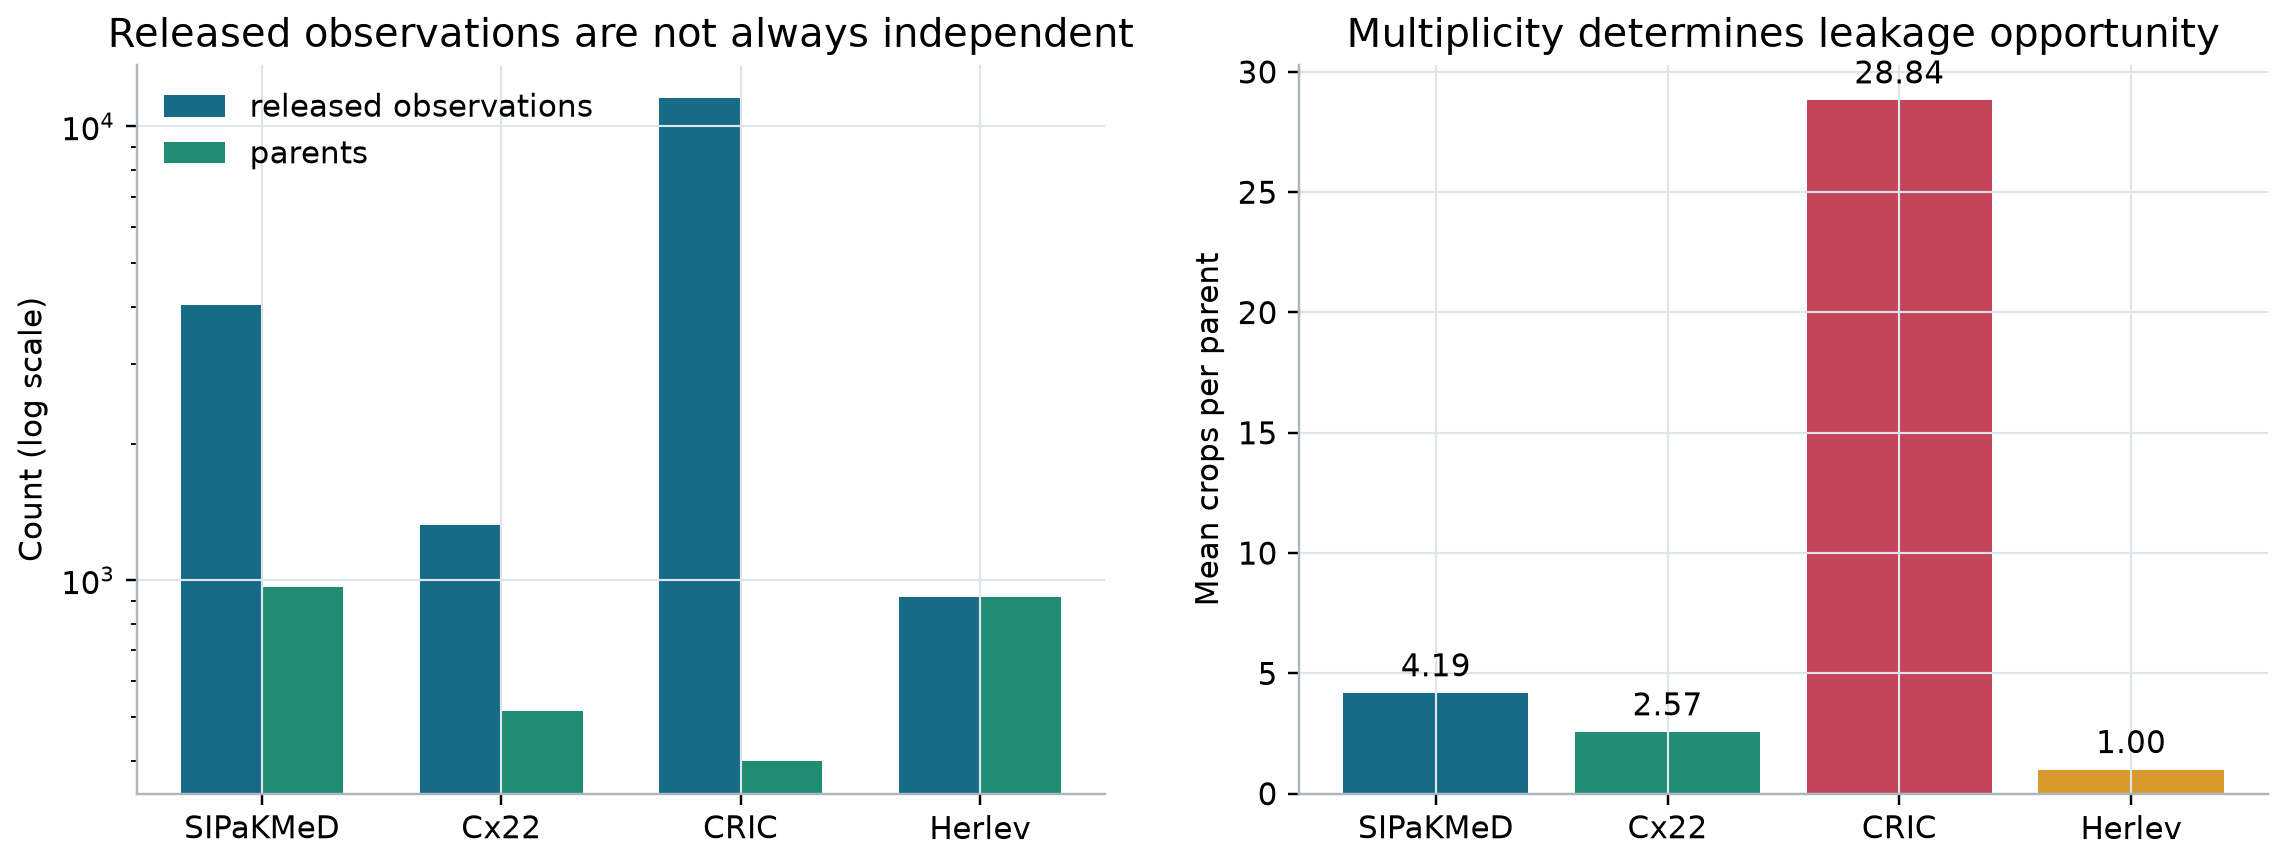
\includegraphics[width=\textwidth]{dataset_scale.png}
\caption{Dataset scale and mean parent multiplicity. The log-scale left panel prevents CRIC's 11,534 observations from visually erasing the smaller datasets.}
\label{fig:dataset-scale}
\end{figure}

\begin{figure}[H]
\centering
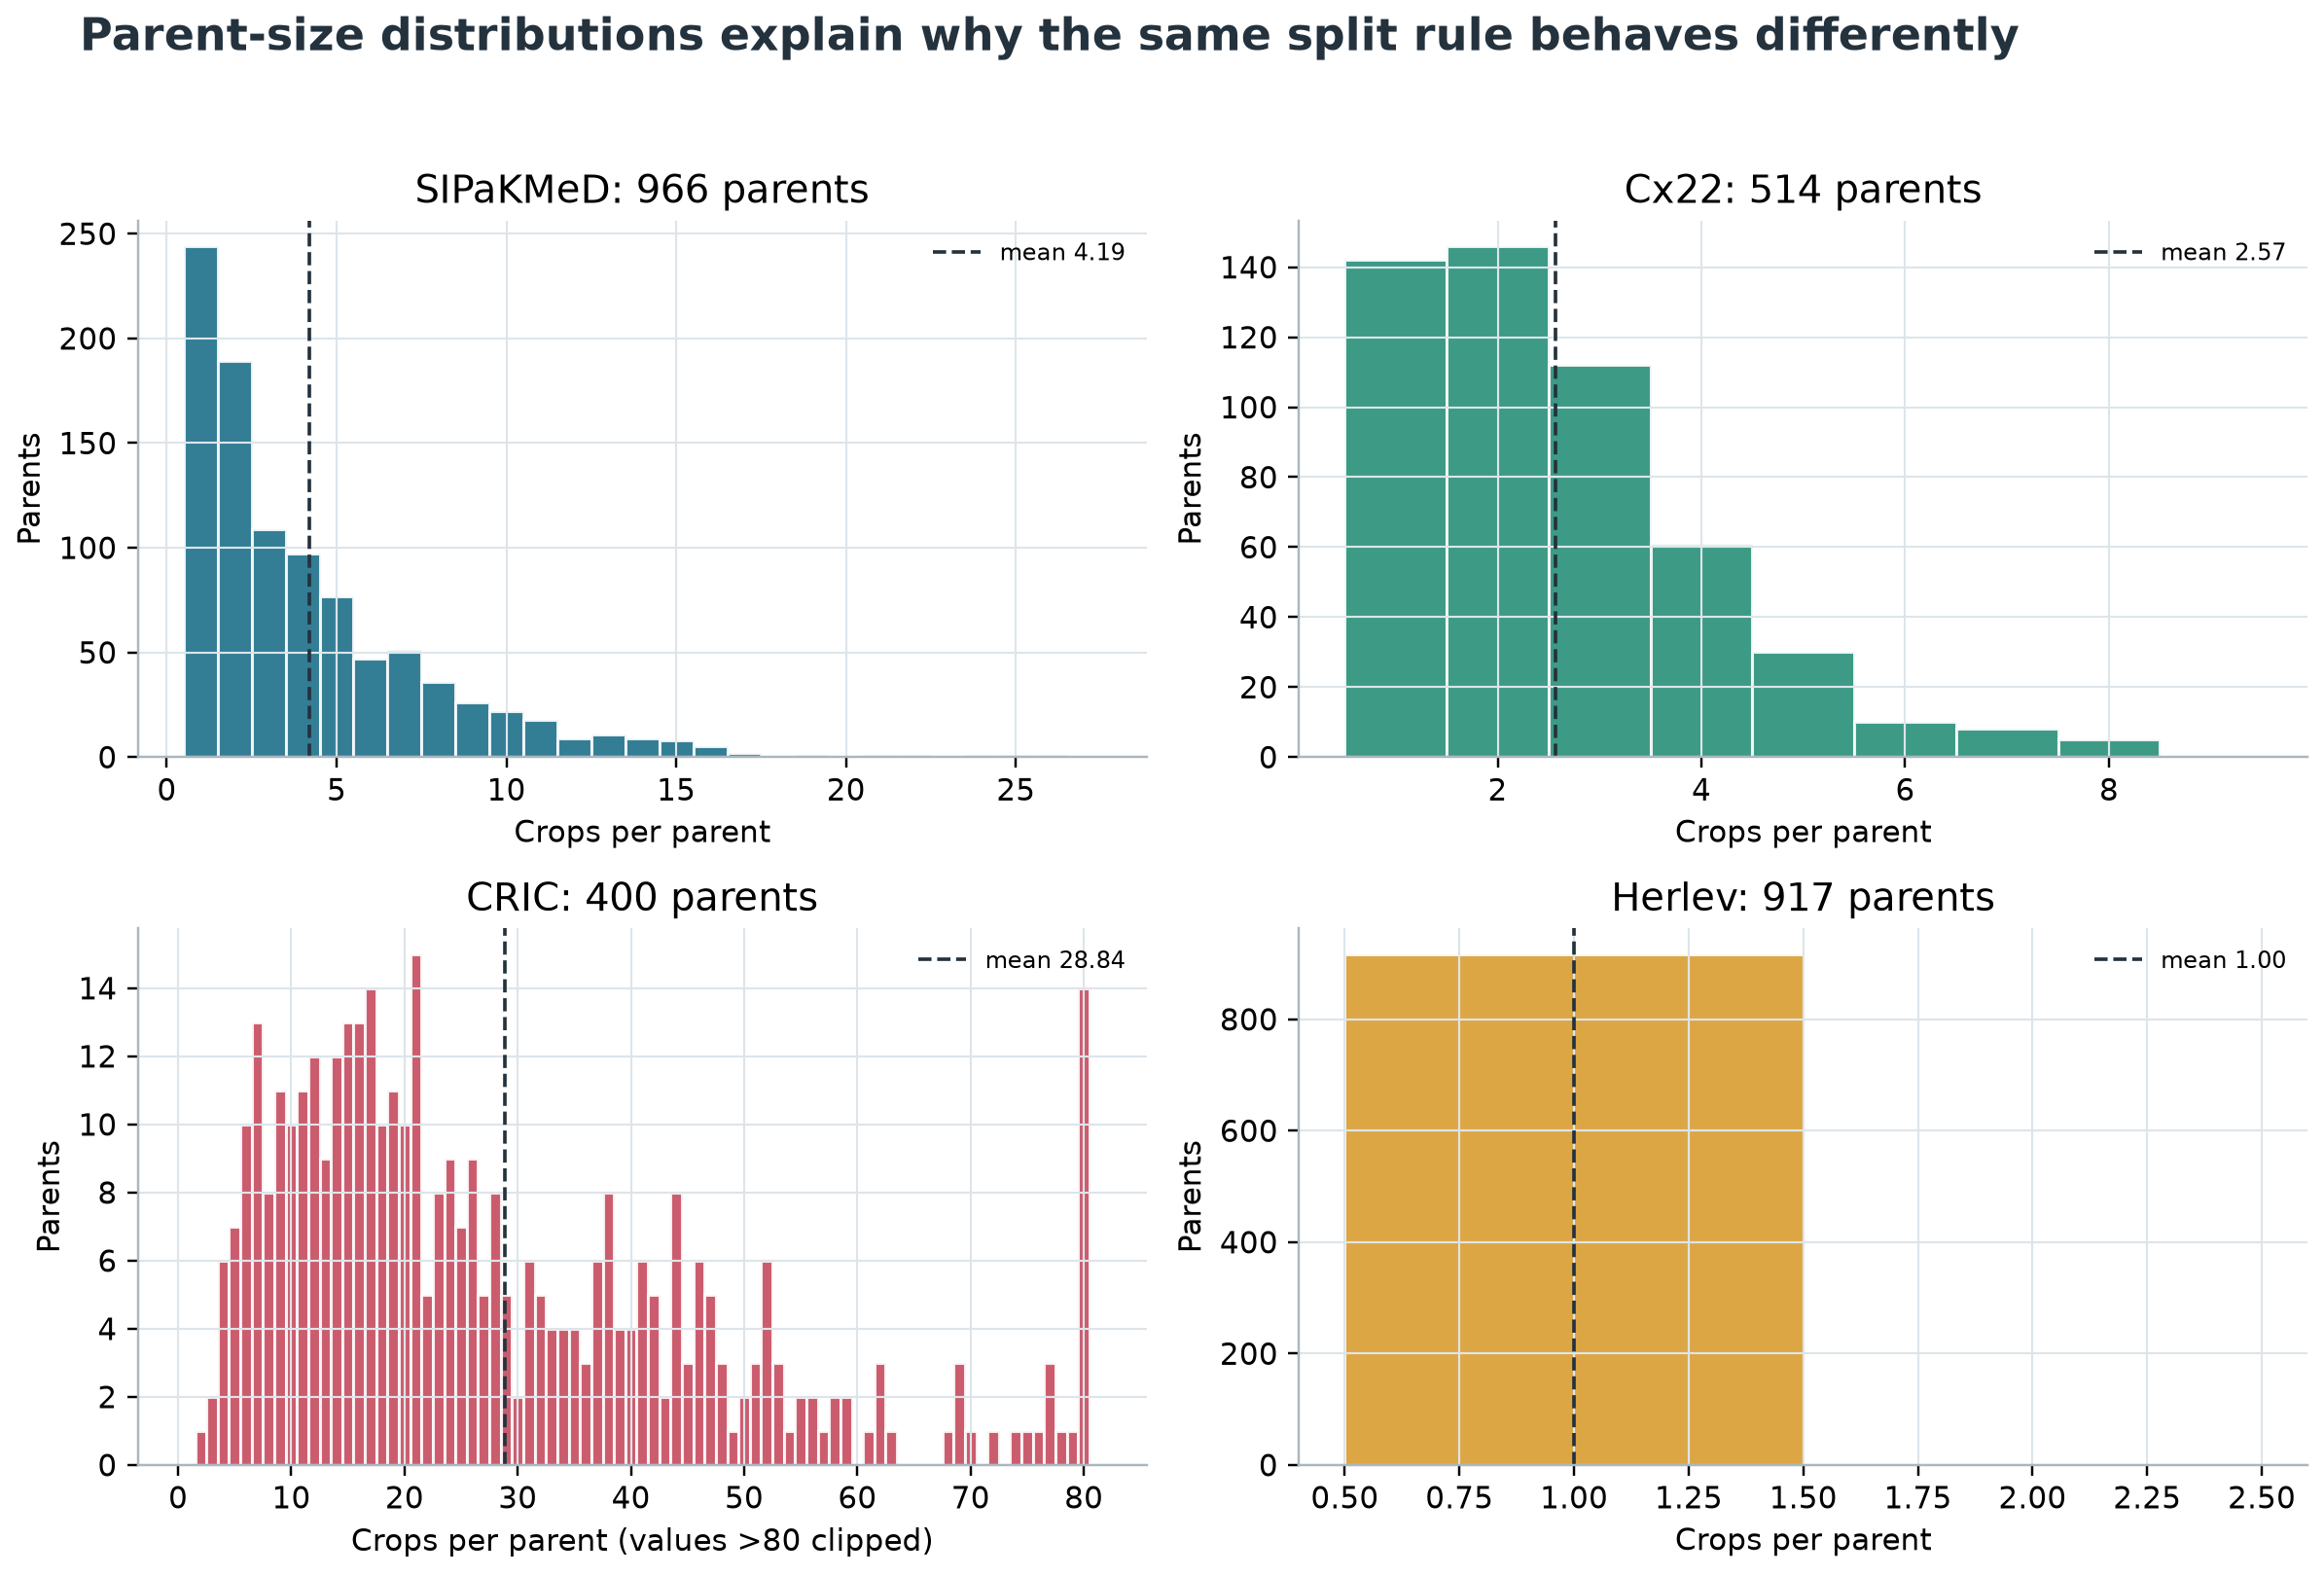
\includegraphics[width=\textwidth]{parent_size_distributions.png}
\caption{Complete parent-size distributions recovered from the Parquet maps. High multiplicity drives the probability that random crop splitting places a parent in both arms.}
\label{fig:parent-distributions}
\end{figure}

\section{SIPaKMeD}

SIPaKMeD contains 4,049 isolated cell images derived from 966 cluster fields~\cite{plissiti2018sipakmed}. The released hierarchy is unusually valuable for an audit: full fields and a \artifact{CROPPED} directory coexist, and crop filenames encode the field identifier. The project uses the cluster field---not the crop file---as the parent.

\begin{table}[H]
\centering
\caption{Independently reconstructed SIPaKMeD class totals in release order.}
\label{tab:sip-classes}
\begin{tabular}{lrrr}
\toprule
Class & Crops & Parents & Crops/parent \\
\midrule
Superficial--Intermediate & 831 & 126 & 6.60 \\
Parabasal & 787 & 108 & 7.29 \\
Koilocytotic & 825 & 238 & 3.47 \\
Metaplastic & 793 & 271 & 2.93 \\
Dyskeratotic & 813 & 223 & 3.65 \\
\midrule
Total & 4,049 & 966 & 4.19 \\
\bottomrule
\end{tabular}
\end{table}

The class order deserves explicit mention because the original planning text swapped the final two names even though its numerical vector was right. The integrity gate exposed that inconsistency, and Amendment 1 corrected it before results existed. This is an example of a check preventing a quiet metadata error.

\section{Cx22 and CCEDD}

Cx22 provides 1,320 generated regions and instance labels, drawing source images from CCEDD~\cite{liu2022cx22}. Three released subsets are involved: Multi-Train, Multi-Test, and Pair. The parent is the named CCEDD source image. Generator metadata provide source name and requested ROI coordinates; the authors' MATLAB generator defines how a source rectangle is clipped, resized, and pasted into a 512-by-512 white canvas.

The official Multi-Train and Multi-Test arms have zero shared parents. Pair is separately released and shares 55 parents with Multi-Test (Jaccard 0.126) and 233 with Multi-Train (Jaccard 0.475). The later model matrix pools all 1,320 observations only as a preregistered stress test of downstream reuse. It is not an accusation that the official authors used a leaking split.

\begin{figure}[H]
\centering
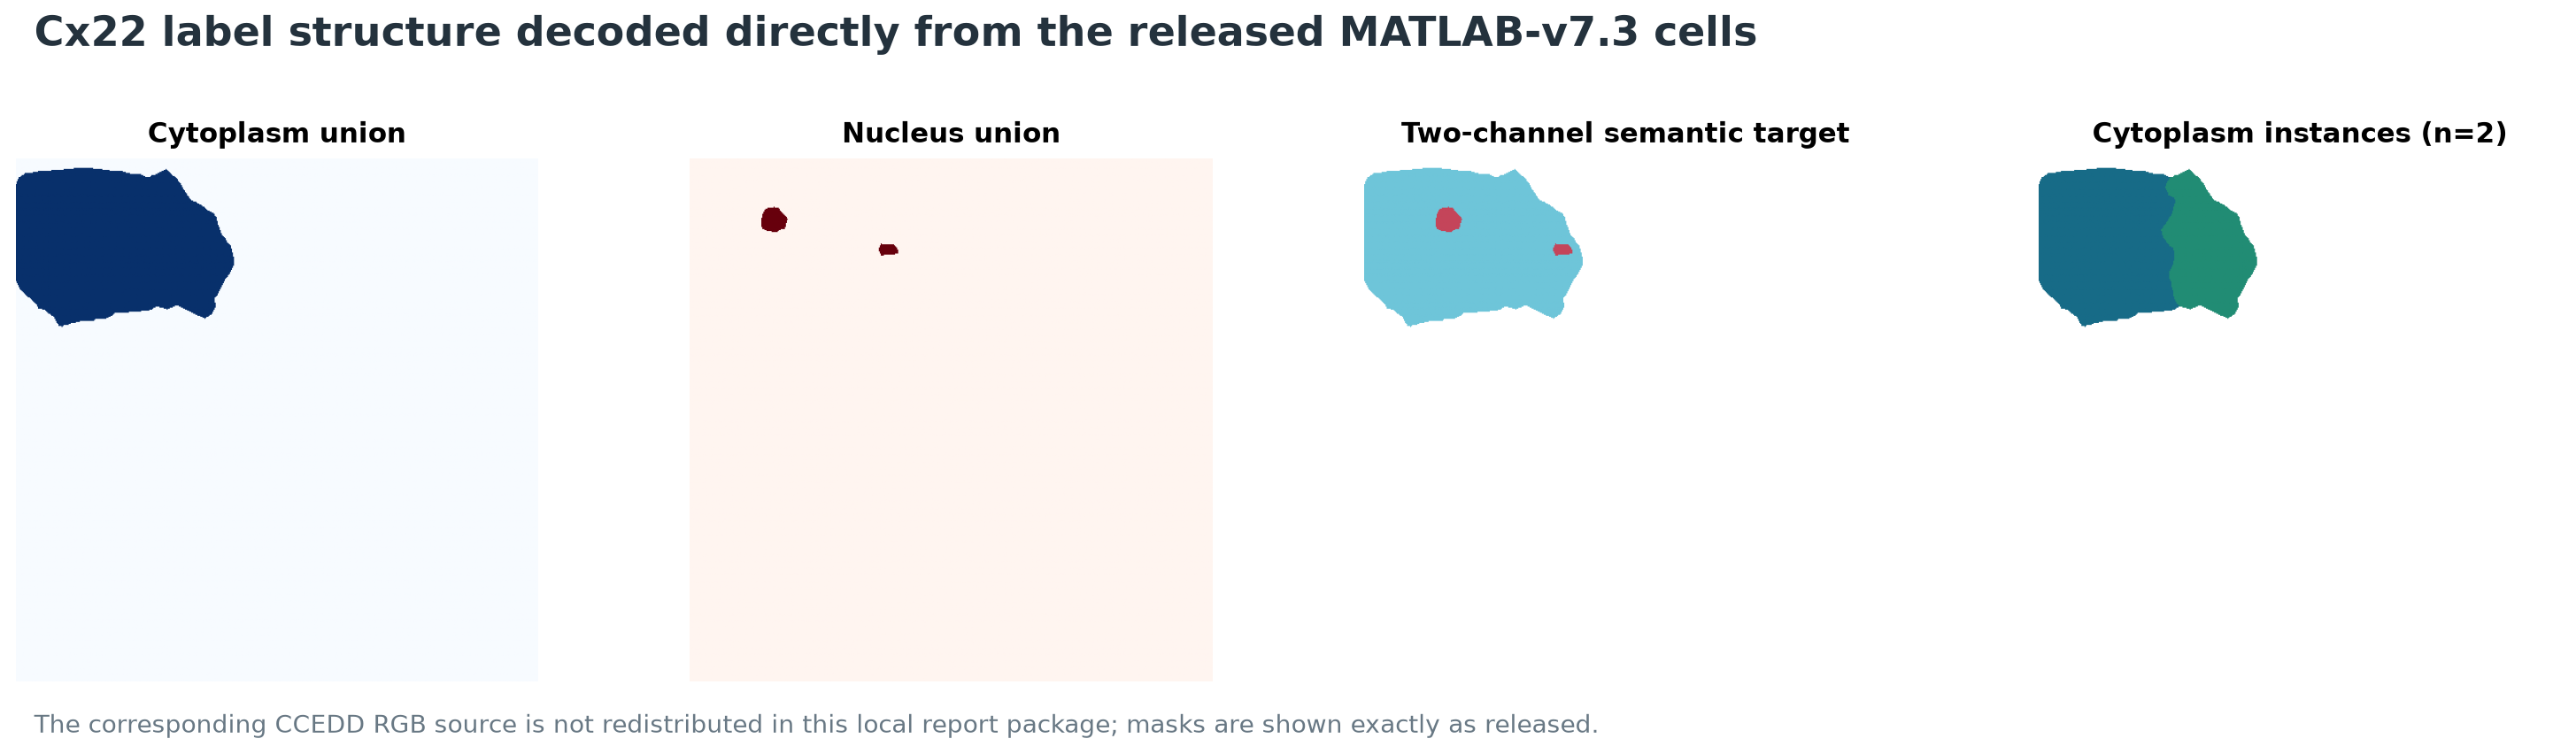
\includegraphics[width=\textwidth]{cx22_label_structure.png}
\caption{One released Cx22 Pair target decoded from the MATLAB-v7.3 structures. Cytoplasm and nucleus unions define two non-exclusive semantic channels; individual cytoplasm masks define the instance task. The CCEDD RGB source is not redistributed in this report.}
\label{fig:cx22-labels}
\end{figure}

\section{CRIC}

CRIC contains 11,534 classified cells associated with 400 source images~\cite{rezende2021cric}. The released classification table supplies source identity and cell coordinates, which makes source-level grouping deterministic. A reliable patient identifier is not present in the released table, so the project does not claim patient-disjoint evaluation. This matters: source-image grouping is stronger than crop grouping but can still be weaker than patient grouping.

\section{Herlev as a structural negative control}

Herlev contains 917 released single-cell images~\cite{jantzen2005pap}. Under the project's declared data unit, each image is one observation and one parent. It therefore has no multi-observation parent structure and must return exactly zero parent straddling. If Herlev showed a nonzero structural effect, the implementation would be wrong. The control passed for all five seeds.

\section{Data-use constraints}

The repository publishes identifiers, coordinates, hashes, split assignments, code, and derived statistics. It does not redistribute raw images. Cx22/CCEDD material is restricted to non-commercial research/education in the declared source manifest, and CCEDD redistribution is prohibited. CRIC and the local Herlev repackaging are declared CC BY 4.0. SIPaKMeD's source notes require citation and experimental use. The complete URL/checksum/terms ledger appears in \cref{tab:data-sources}.

\chapter{System architecture and fail-closed philosophy}

\section{Pipeline}

\begin{figure}[H]
\centering
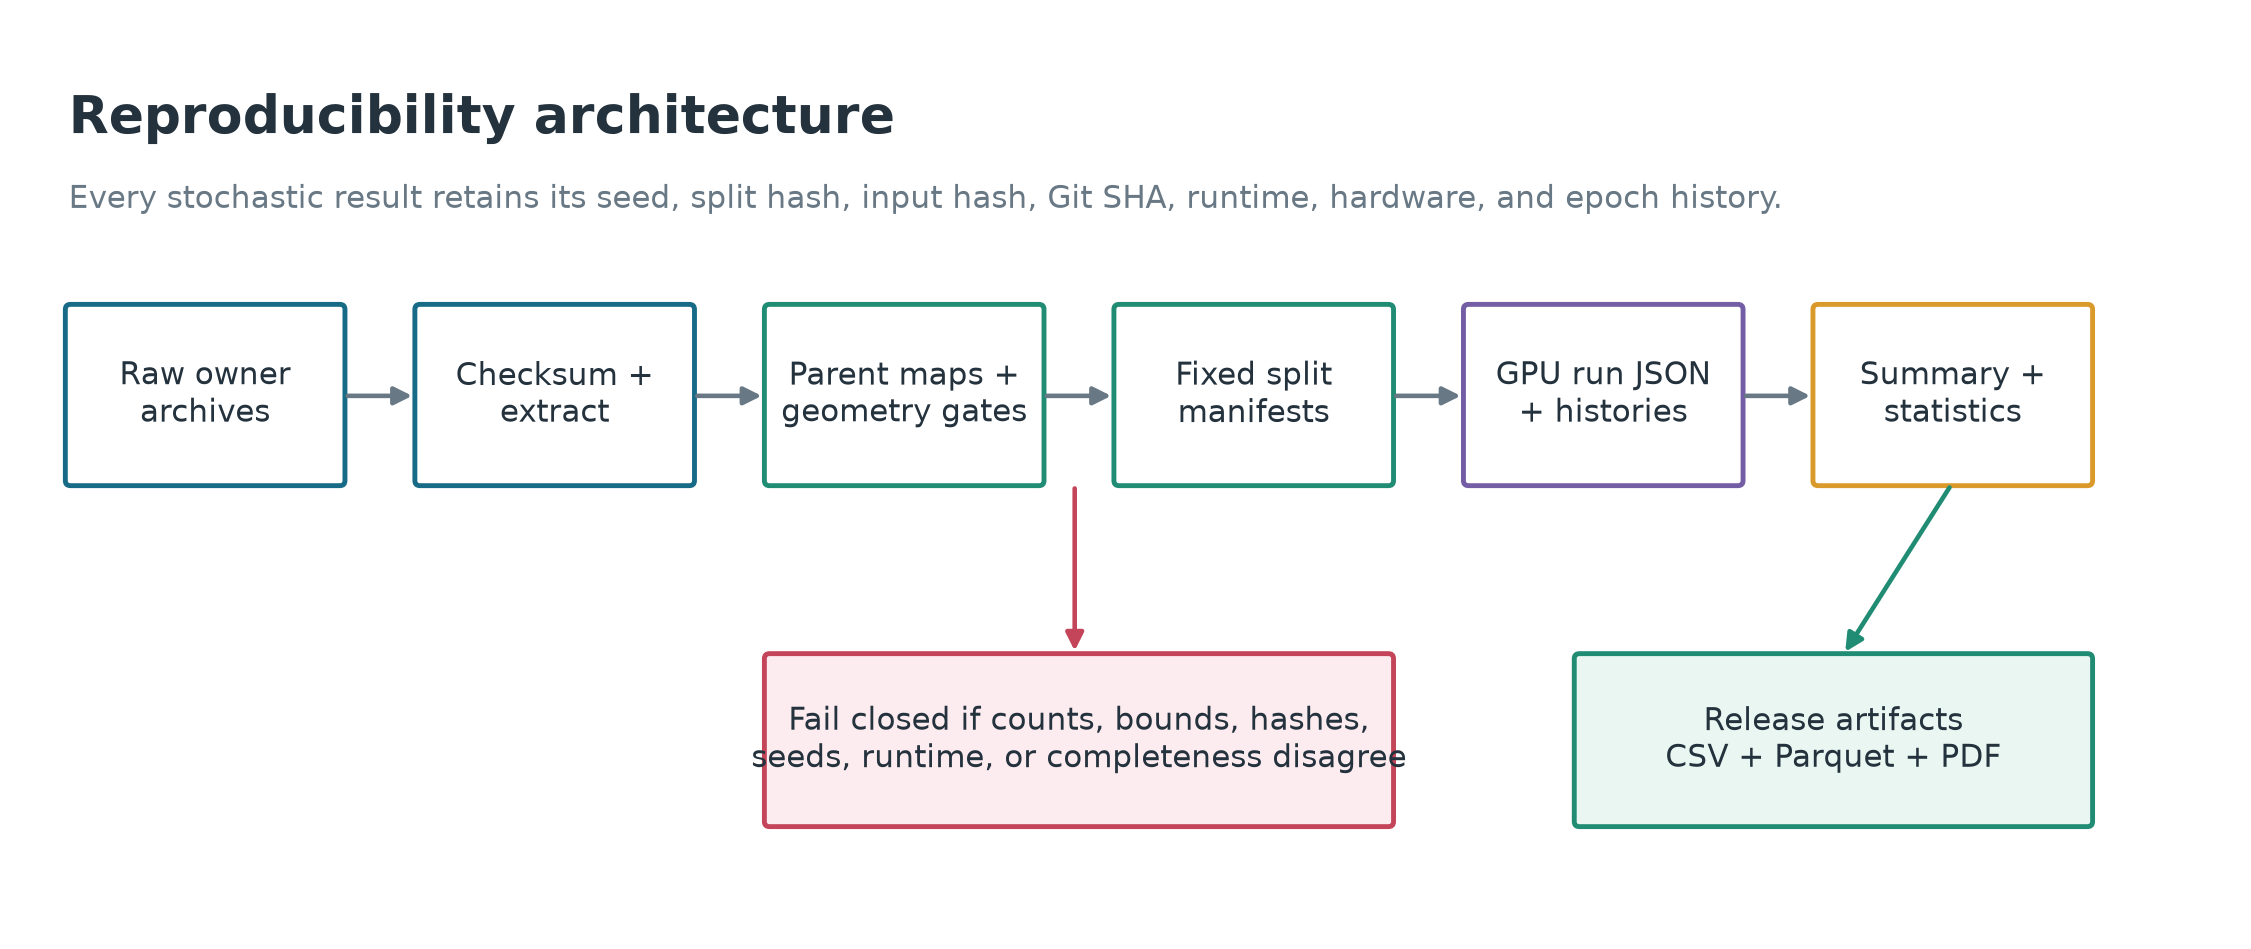
\includegraphics[width=\textwidth]{reproducibility_pipeline.png}
\caption{Reproducibility architecture. Deterministic provenance and split artifacts gate the stochastic GPU experiments, and every final result carries the hashes needed to reconnect it to its inputs.}
\label{fig:repro-pipeline}
\end{figure}

The system deliberately separates three artifact layers:
\begin{enumerate}[leftmargin=2em]
  \item \textbf{Canonical identity:} exact or released parent IDs used to construct splits.
  \item \textbf{Independent audit:} image-matched parent IDs, boxes, confidence, runner-up margin, and an auxiliary diagnostic flag.
  \item \textbf{Sensitivity grouping:} P3 connected-component IDs built from thresholded cross-parent near-duplicate candidates.
\end{enumerate}

Keeping these layers separate prevents a lower-confidence image match from overwriting an exact filename identity. It also prevents a conservative pHash/dHash candidate from being narrated as a proven duplicate.

\section{Core artifact schemas}

The canonical SIPaKMeD map records \artifact{crop_id}, \artifact{parent_id}, \artifact{class_name}, paths, recovery method, and confidence. Branch B adds $x,y,w,h$, crop and parent dimensions, coarse and refined NCC, second-best confidence, margin, method, and diagnostic \artifact{accepted}. P3 adds \artifact{p3_group_id}. Split CSVs record \artifact{crop_id}, \artifact{parent_id}, \artifact{partition}, \artifact{protocol}, and \artifact{seed}.

Every neural result JSON records task, architecture, protocol/mode, seed, primary and secondary metrics, train/test counts, hyperparameters, exact split/input hashes, Git SHA, timestamps, elapsed time, visible GPU, platform and library versions, and full epoch history. This is more useful than a final number alone: it permits matrix completeness checks, runtime analysis, and learning-curve reconstruction without checkpoints.

\section{Fail-closed algorithm}

\begin{lstlisting}[style=cyto,caption={Conceptual fail-closed workflow.},label={lst:algorithm}]
for each released dataset:
    recover exact/released parent identity
    if an independent recovery branch exists:
        recover parent and bounding box without consulting branch A
        require >= 99% A/B agreement
    require one parent per observation
    require all boxes contained and all totals exact

construct P1, P1-prime, P2, and P3 for every fixed seed
measure structural and literal overlap
run probe/classifier/segmenter matrix with bounded GPUs

before summarizing:
    require every registered cell and seed exactly once
    require split hashes, runtime versions, and sample counts
    pair comparisons by seed
    attach an effect size and interval to every p-value
    apply BH over the entire declared family once

if any required evidence is absent:
    emit FAIL or PENDING; never infer PASS
\end{lstlisting}

\chapter{Exact provenance recovery}

\section{SIPaKMeD Branch A: filename hierarchy}

Branch A parses the released directory and filename convention. For example, \artifact{im_Dyskeratotic/CROPPED/001_03.bmp} maps to parent \artifact{Dyskeratotic/001}. This route is deterministic, fast, and used for the canonical split map. Its weakness is that a parsing bug could produce internally tidy but wrong identifiers. That is why Branch B was required.

\section{SIPaKMeD Branch B: independent content matching}

For crop $x$ and candidate parent region $r$, normalized cross-correlation is
\begin{equation}
\operatorname{NCC}(x,r)=
\frac{\sum_u(x_u-\bar{x})(r_u-\bar{r})}
{\sqrt{\sum_u(x_u-\bar{x})^2}\sqrt{\sum_u(r_u-\bar{r})^2}}.
\end{equation}

Branch B never uses Branch A's parent assignment in the query. It ranks every same-class parent at quarter resolution, refines the five best candidates at full resolution, and records the winning location as a bounding box. A multiscale fallback exists only for unresolved cases. Matching is bounded by class working sets so the complete parent image collection does not have to remain in memory.

\begin{figure}[H]
\centering
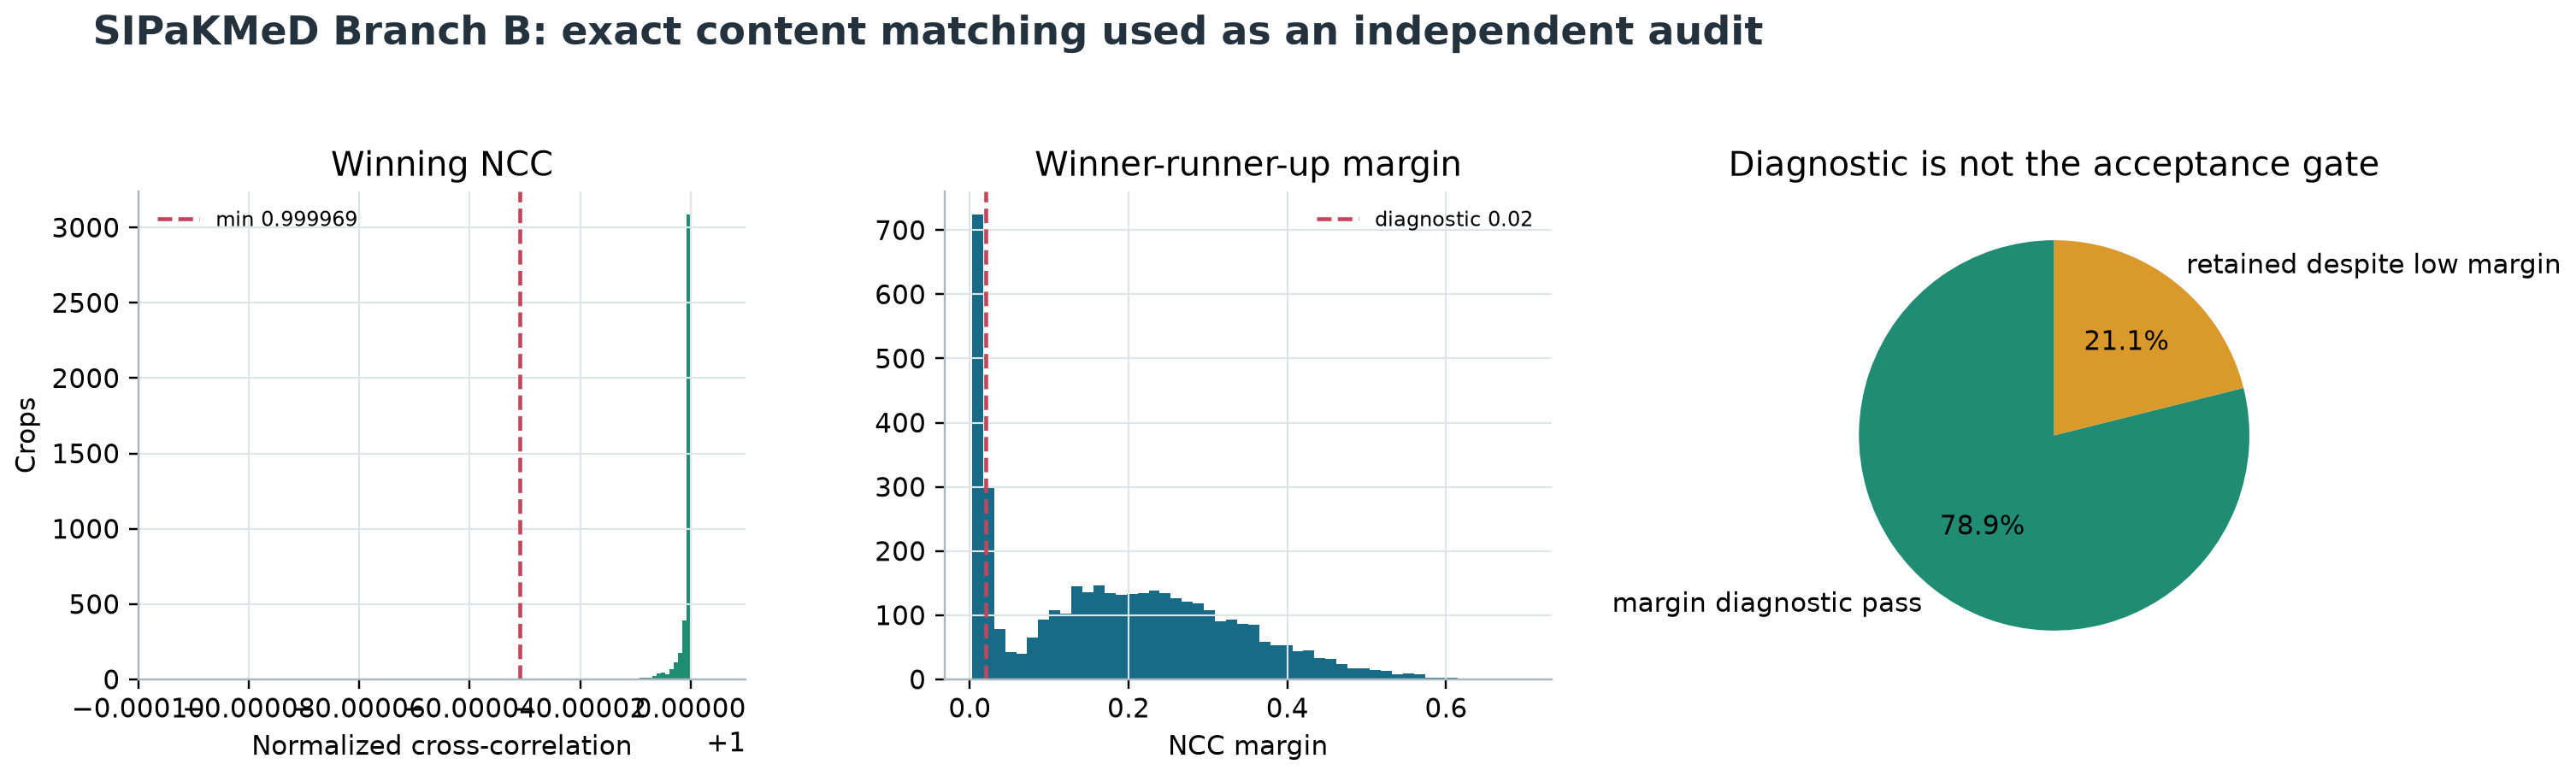
\includegraphics[width=\textwidth]{provenance_diagnostics.png}
\caption{Branch-B diagnostics. The minimum winning NCC is 0.999969. The 0.02 runner-up-margin rule is intentionally only a diagnostic: 3,195 crops pass it and 854 do not, yet all rows agree with Branch A and all boxes remain contained.}
\label{fig:provenance-diagnostics}
\end{figure}

\begin{figure}[H]
\centering
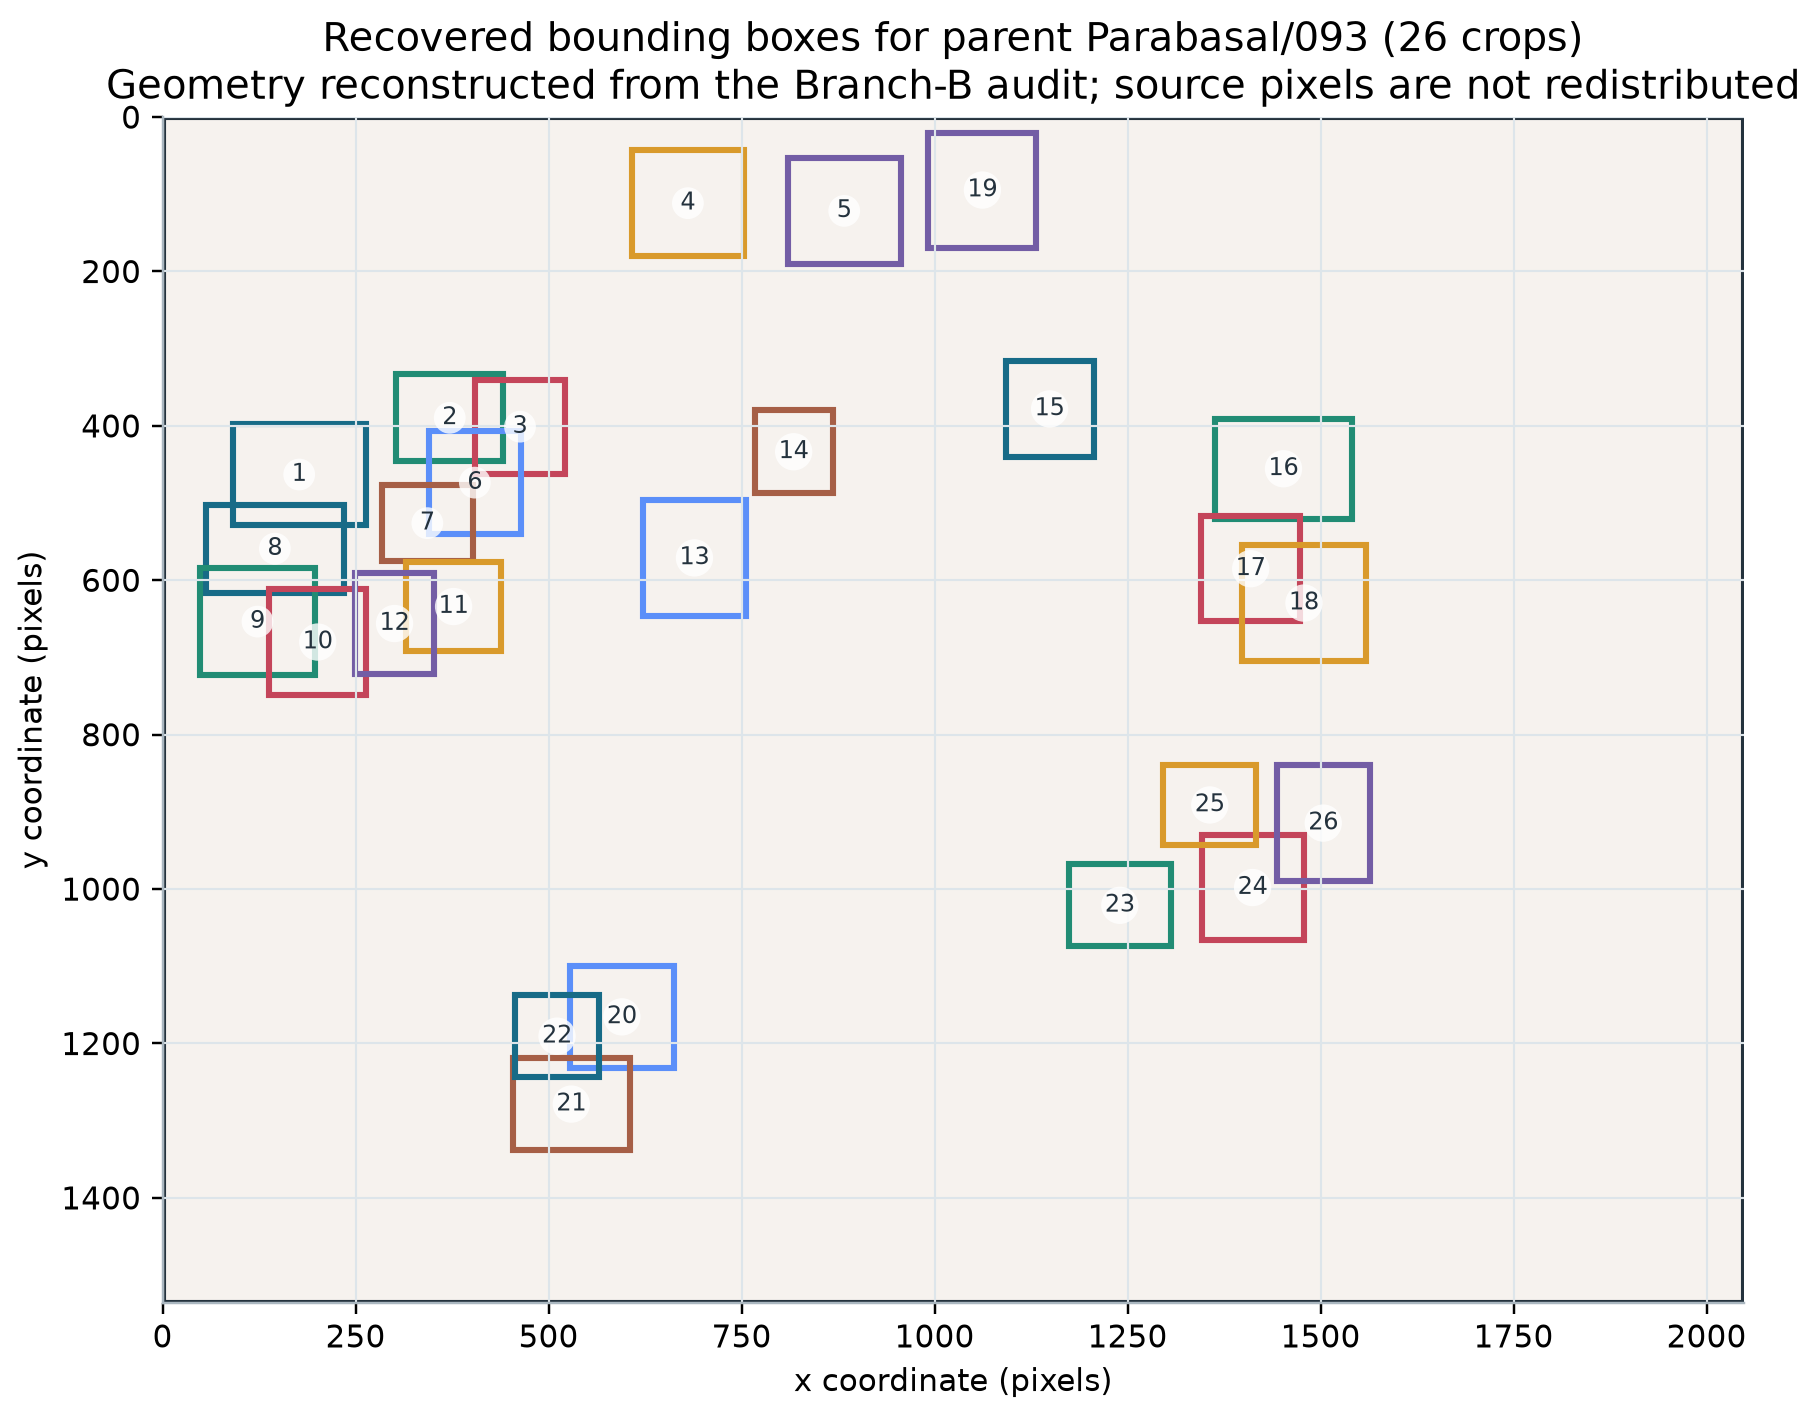
\includegraphics[width=0.77\textwidth]{recovered_bbox_example.png}
\caption{A real recovered-coordinate example for the parent with the largest crop count. Only rectangle geometry is displayed; source pixels are not redistributed. Overlapping rectangles make literal source-pixel sharing possible.}
\label{fig:bboxes}
\end{figure}

\section{Why the auxiliary acceptance flag is false for many correct rows}

The \artifact{accepted} field in Branch B encodes a conservative confidence-plus-margin diagnostic. It is not the registered provenance acceptance outcome. Many microscope fields contain visually repetitive background, so a correct near-perfect winner can have another near-perfect candidate. Substituting this diagnostic for the registered 99\% cross-branch agreement rule would discard 854 correctly mapped crops after looking at an arbitrary margin. The project instead retains every row and exposes the ambiguity measure.

\section{Cx22, CRIC, and Herlev recovery}

Cx22 uses source names and ROI coordinates decoded from the authors' three MATLAB generator releases. Every source resolves against the declared 686-image CCEDD set, and rare edge-touching requested boxes are clipped exactly as the generator code specifies. The released Cx22 archives contain generator metadata and masks rather than a second independent RGB crop array, so an A/B image-content branch cannot be constructed from the public package alone. Applicable checks are source existence, exact metadata decoding, generator geometry, bounds, and subset overlap.

CRIC uses the released classifications table: source-image identity and coordinates directly define the map. Herlev assigns each released cell to itself. Neither route pretends to recover unavailable patient identity.

\section{Verification outcome}

\begin{table}[H]
\centering
\caption{Provenance gates.}
\label{tab:provenance-gates}
\begin{tabularx}{\textwidth}{lrrXl}
\toprule
Dataset & Observations & Parents & Applied evidence & Outcome \\
\midrule
SIPaKMeD & 4,049 & 966 & 4,049/4,049 A/B agreement; 4,049 contained boxes; exact class totals & \pass \\
Cx22 & 1,320 & 514 & generator names/ROIs; 686 sources resolve; 1,320 contained clipped boxes & \pass \\
CRIC & 11,534 & 400 & released source identities and coordinates; no patient-ID claim & \pass \\
Herlev & 917 & 917 & one released cell per parent & \pass \\
\bottomrule
\end{tabularx}
\end{table}

No observation was excluded. The five SIPaKMeD parent counts are exactly 126/108/238/271/223 in corrected release order. All crop counts sum to 4,049.

\chapter{Split protocols and structural leakage}

\section{Why four protocols are needed}

\begin{figure}[H]
\centering
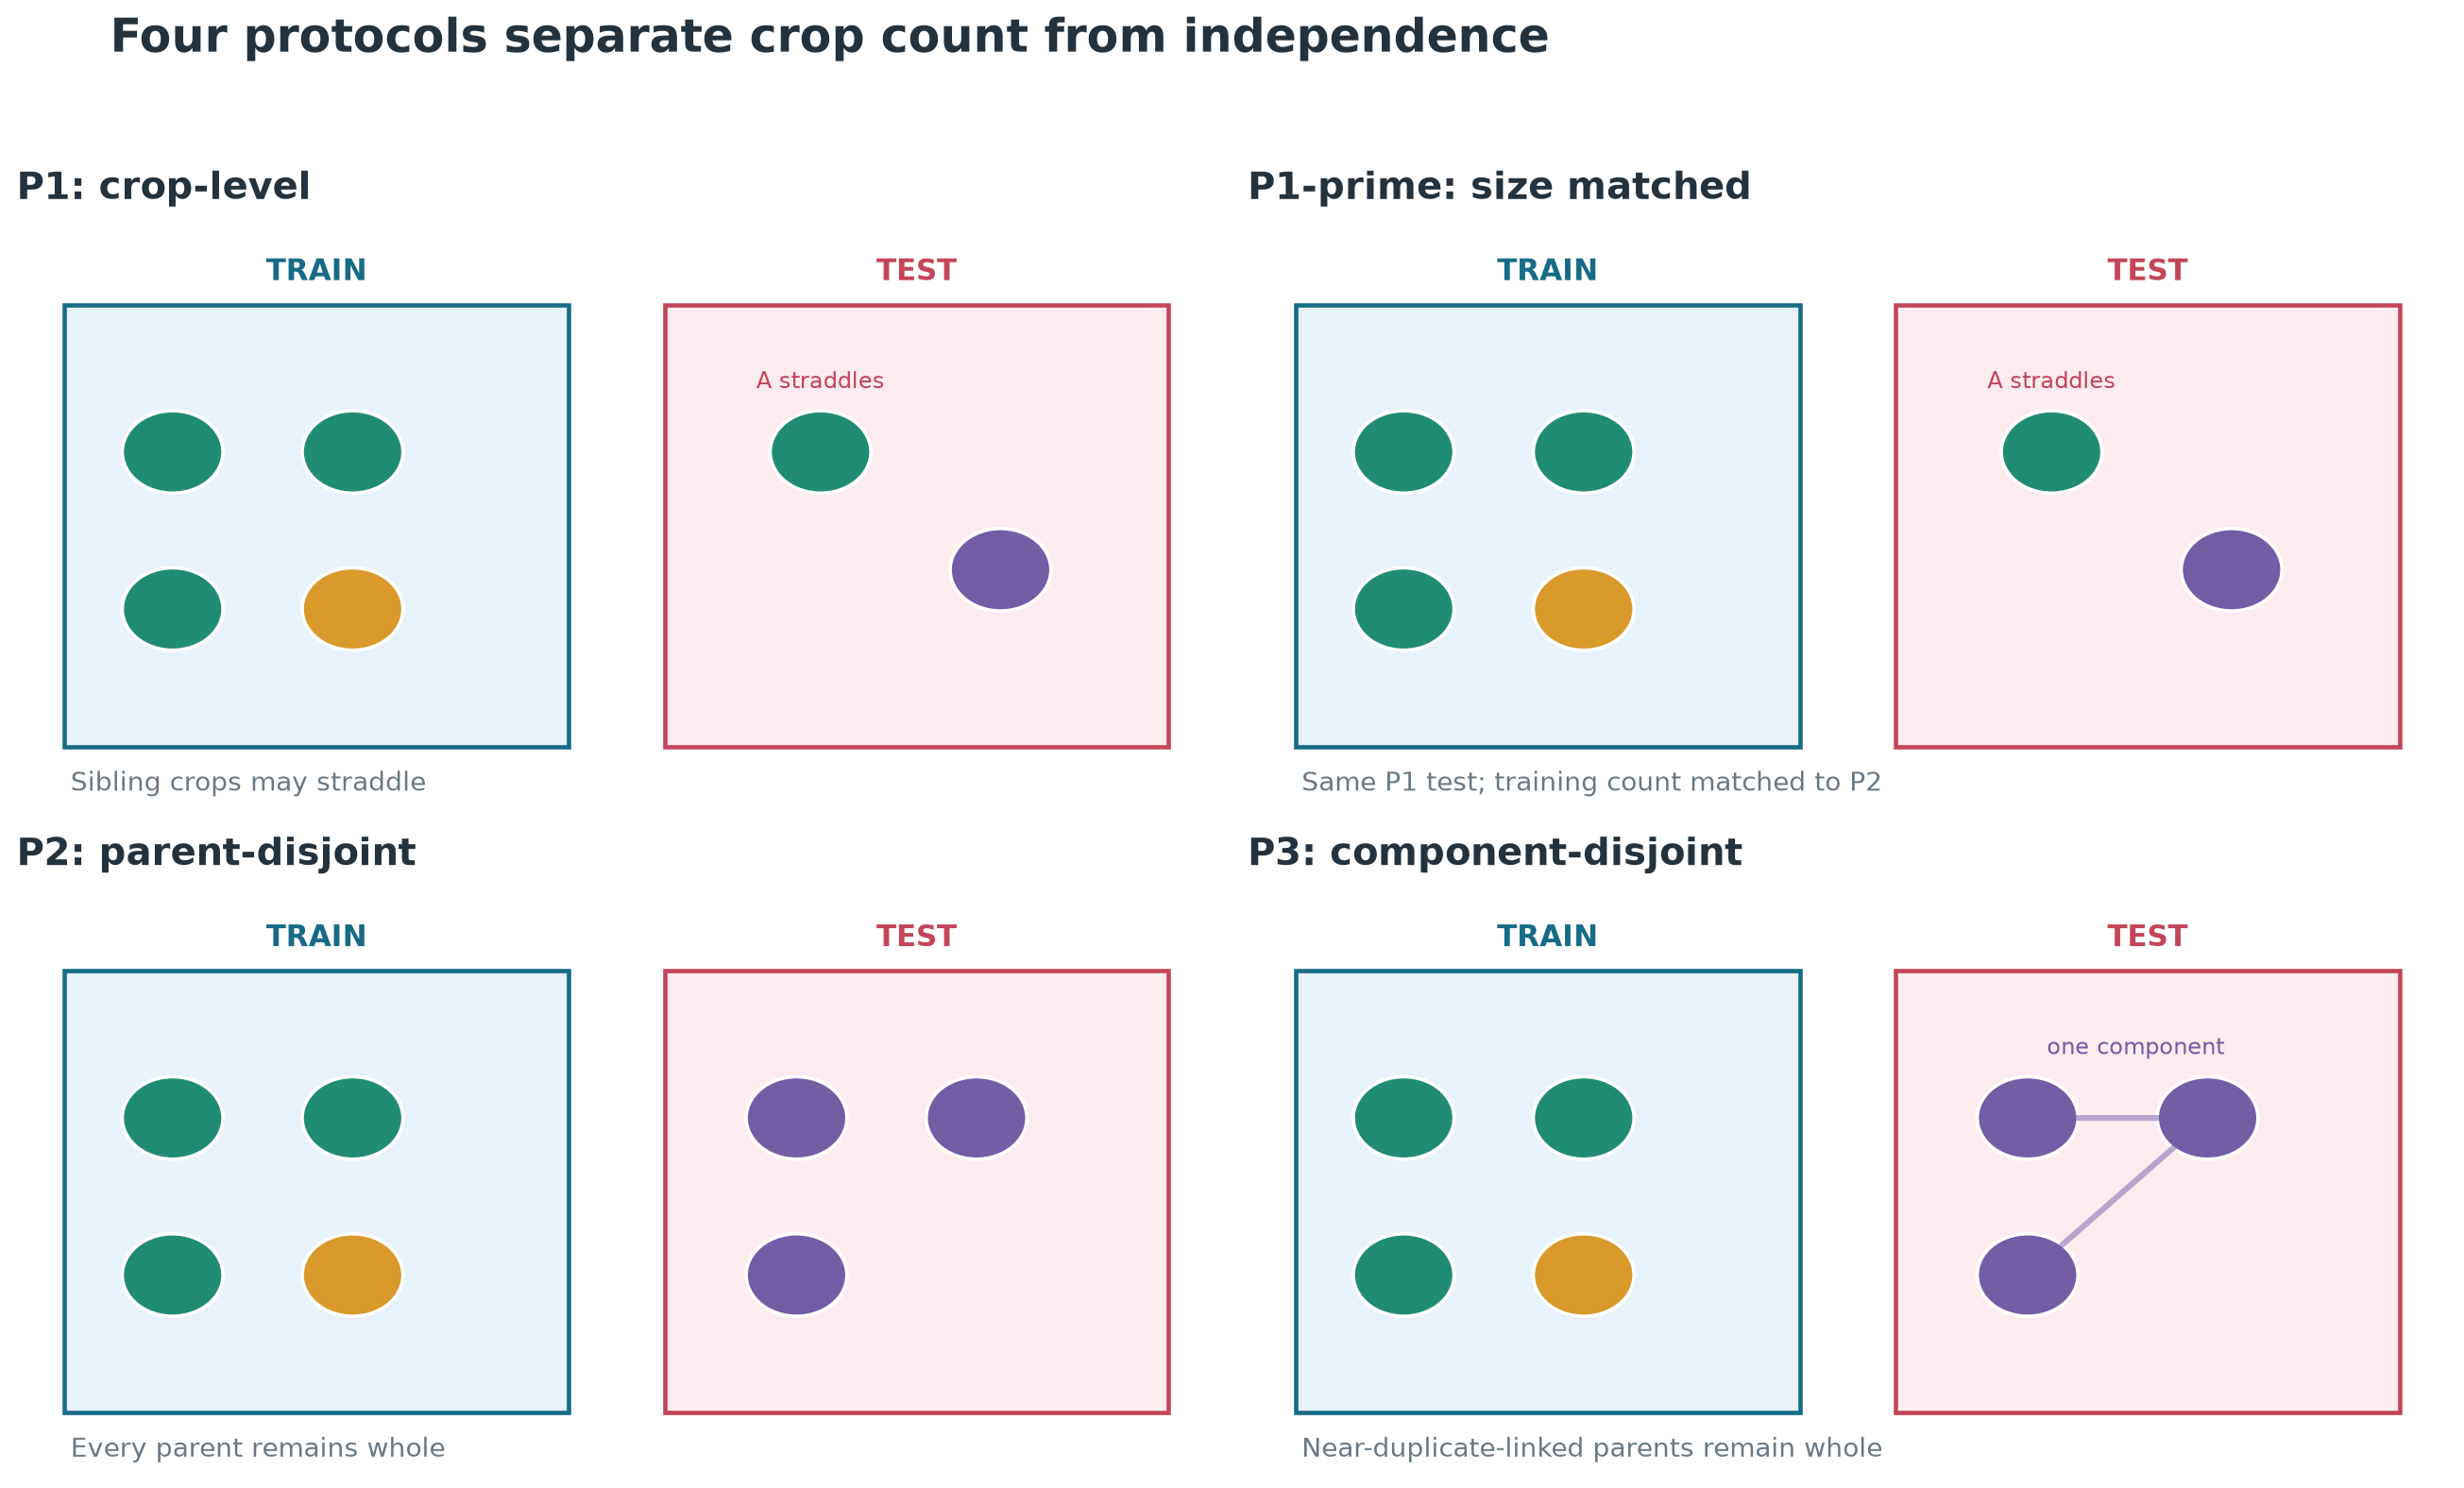
\includegraphics[width=\textwidth]{split_protocols.png}
\caption{The four protocols. P1 asks what common crop splitting shares. P1-prime holds its test set but matches the P2 training count. P2 groups exact parents. P3 groups whole near-duplicate-linked parent components.}
\label{fig:protocols}
\end{figure}

All splits use an 80:20 target and the five fixed seeds. P1 is class-stratified at crop level. P1-prime retains P1's test observations and downsamples only its training observations to exactly the P2 training count, as closely class-balanced as integer counts permit. P2 uses group-aware allocation by exact parent. P3 repeats parent-disjoint allocation after cross-parent candidate links are collapsed into connected components.

On the frozen SIPaKMeD environment, P2 contains 3,239 train and 810 test crops for every seed. P1 already has exactly those counts, so P1-prime is identical to P1. This is not a redundant hidden comparison: it shows that the primary P1--P2 difference cannot be attributed to a larger P1 training set in this implementation.

\section{Analytic straddle probability}

For a parent with $k$ crops independently assigned to training with probability 0.8 and test with probability 0.2, the only non-straddling outcomes are ``all train'' and ``all test.'' Hence
\begin{align}
P(\text{no straddle}\mid k) &= 0.8^k+0.2^k,\\
P(\text{straddle}\mid k) &= 1-0.8^k-0.2^k.
\end{align}
For a dataset with parent crop counts $k_1,\dots,k_m$, the analytic expectation is
\begin{equation}
\bar{P}_{\text{straddle}}=\frac{1}{m}\sum_{j=1}^{m}\left(1-0.8^{k_j}-0.2^{k_j}\right).
\end{equation}

The exact class-stratified fixed-size splitter is not perfectly independent Bernoulli assignment. Therefore the analytic quantity is checked against a 10,000-allocation Monte Carlo interval generated with the actual count vector and allocation rule.

\begin{figure}[H]
\centering
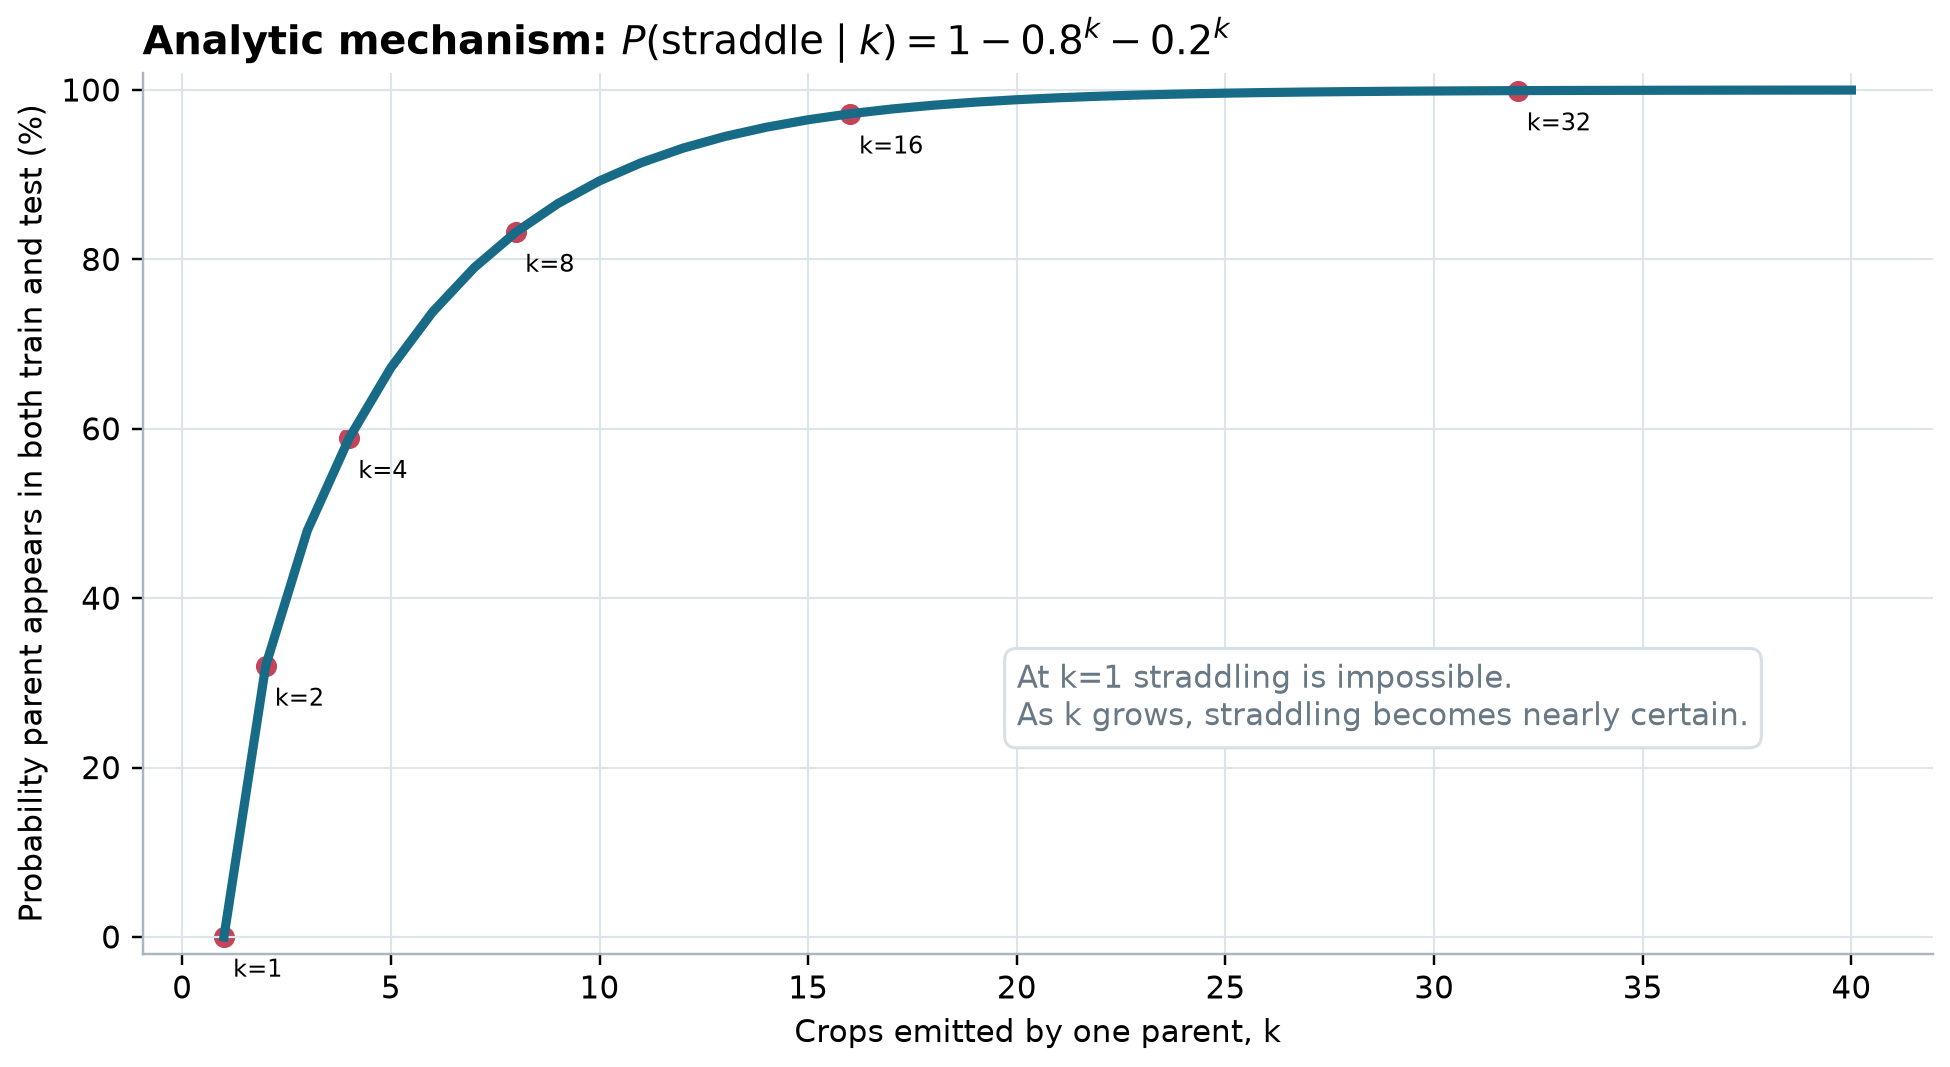
\includegraphics[width=0.87\textwidth]{straddle_probability.png}
\caption{The analytic mechanism. A one-crop parent cannot straddle; a high-multiplicity parent almost certainly straddles under independent 80:20 crop allocation.}
\label{fig:straddle-curve}
\end{figure}

\section{Structural endpoints}

Let $G_{\mathrm{tr}}$ and $G_{\mathrm{te}}$ be training and test parent sets, and let $T$ be the test observations. The parent-straddle fraction and leaked-test-observation fraction are
\begin{equation}
L_p=\frac{|G_{\mathrm{tr}}\cap G_{\mathrm{te}}|}{|G|},\qquad
L_c=\frac{1}{|T|}\sum_{x\in T}\mathbf{1}\{g(x)\in G_{\mathrm{tr}}\}.
\end{equation}

\begin{table}[H]
\centering
\caption{Structural leakage. Stochastic values are mean $\pm$ sample SD over five seeds.}
\label{tab:structural}
\resizebox{\textwidth}{!}{%
\begin{tabular}{lrrrrrr}
\toprule
Dataset & Crops & Parents & Analytic P1 straddle & Observed P1 straddle & P1 test with train parent & P2/P3 straddle \\
\midrule
SIPaKMeD & 4,049 & 966 & 44.83\% & 45.63$\pm$1.04\% & 92.62$\pm$0.40\% & 0.00$\pm$0.00\% \\
Cx22 & 1,320 & 514 & 33.93\% & 34.01$\pm$1.10\% & 85.23$\pm$3.51\% & 0.00$\pm$0.00\% \\
CRIC & 11,534 & 400 & 94.88\% & 94.35$\pm$1.10\% & 99.97$\pm$0.08\% & 0.00$\pm$0.00\% \\
Herlev & 917 & 917 & 0.00\% & 0.00$\pm$0.00\% & 0.00$\pm$0.00\% & 0.00$\pm$0.00\% \\
\bottomrule
\end{tabular}}
\end{table}

\begin{figure}[H]
\centering
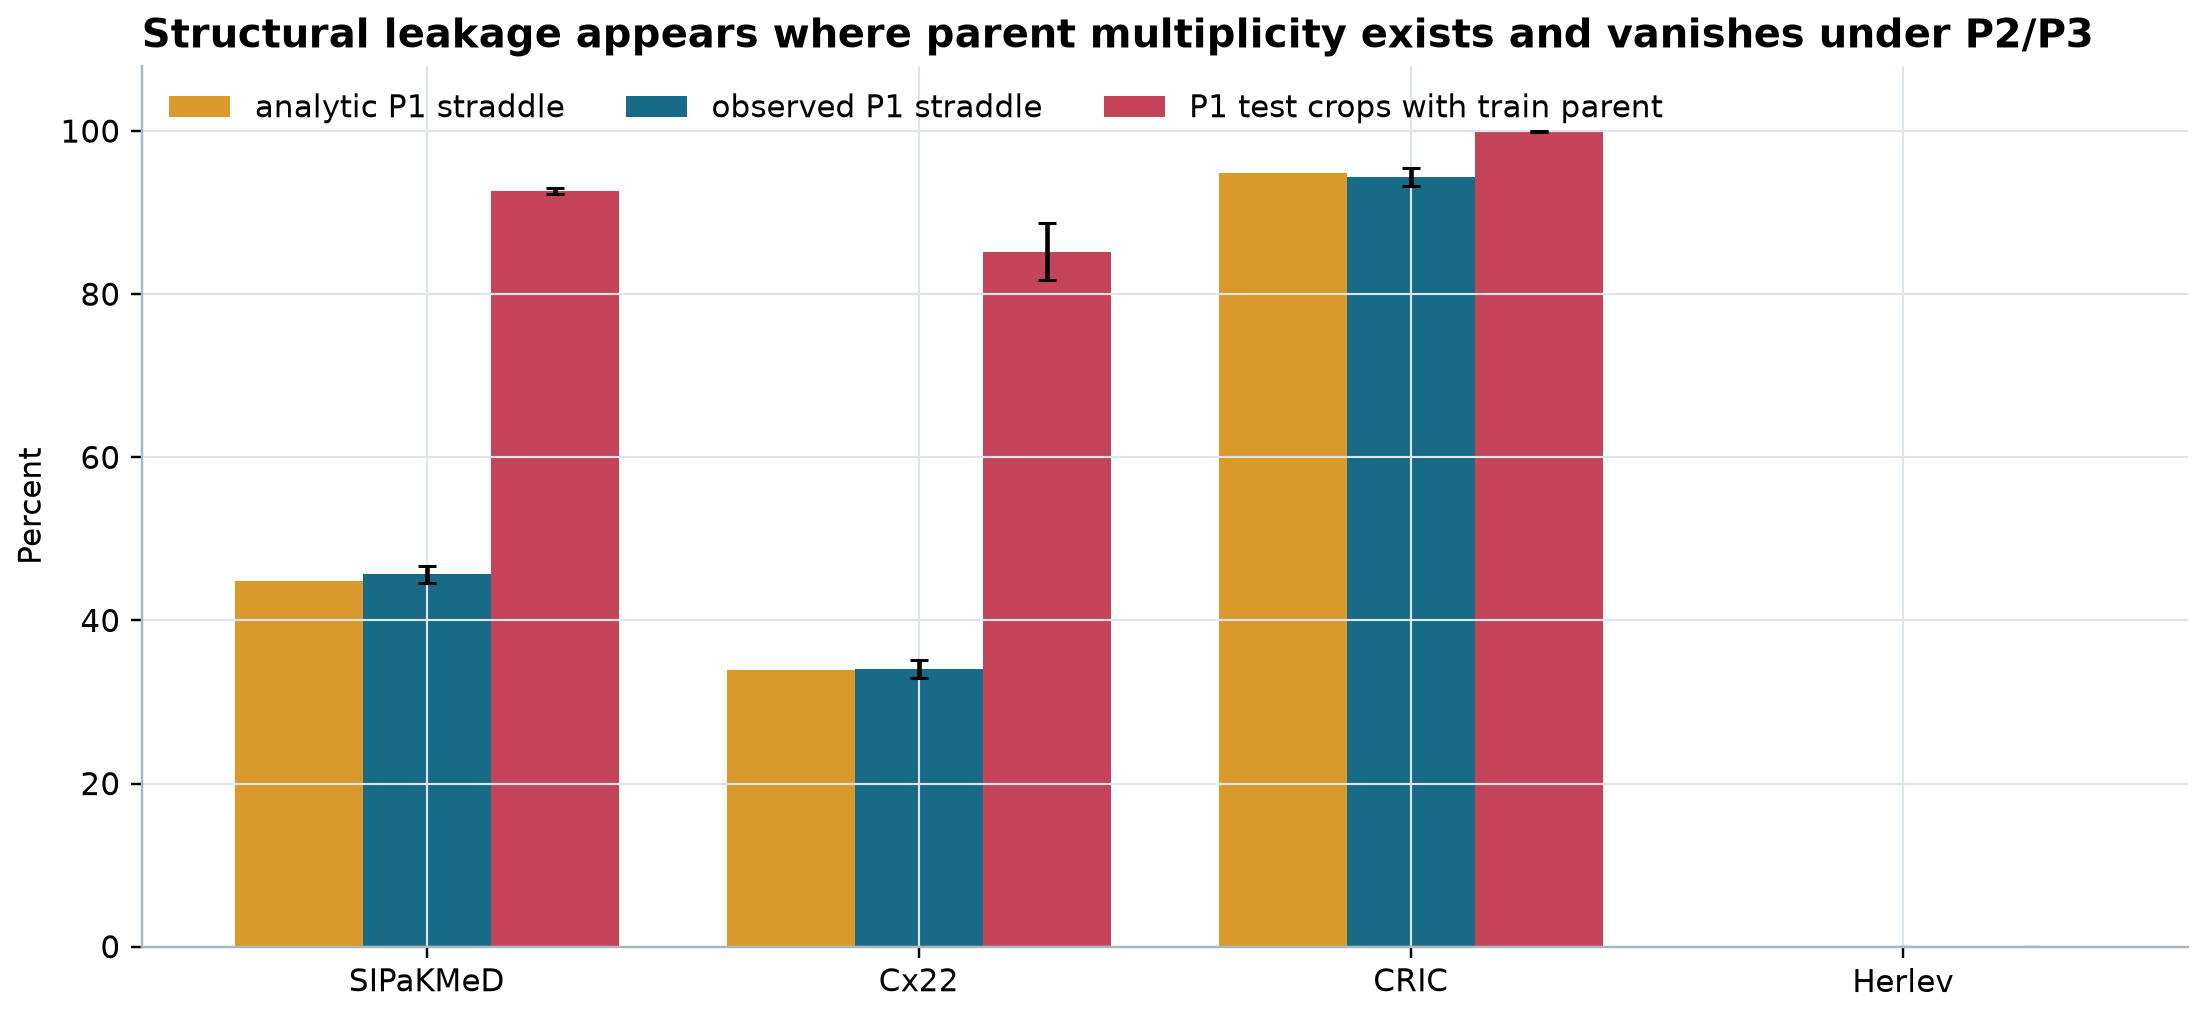
\includegraphics[width=\textwidth]{structural_results.png}
\caption{Analytic and observed leakage. P2 and P3 are omitted from the bars because both are exactly zero on all four datasets.}
\label{fig:structural-results}
\end{figure}

\begin{figure}[H]
\centering
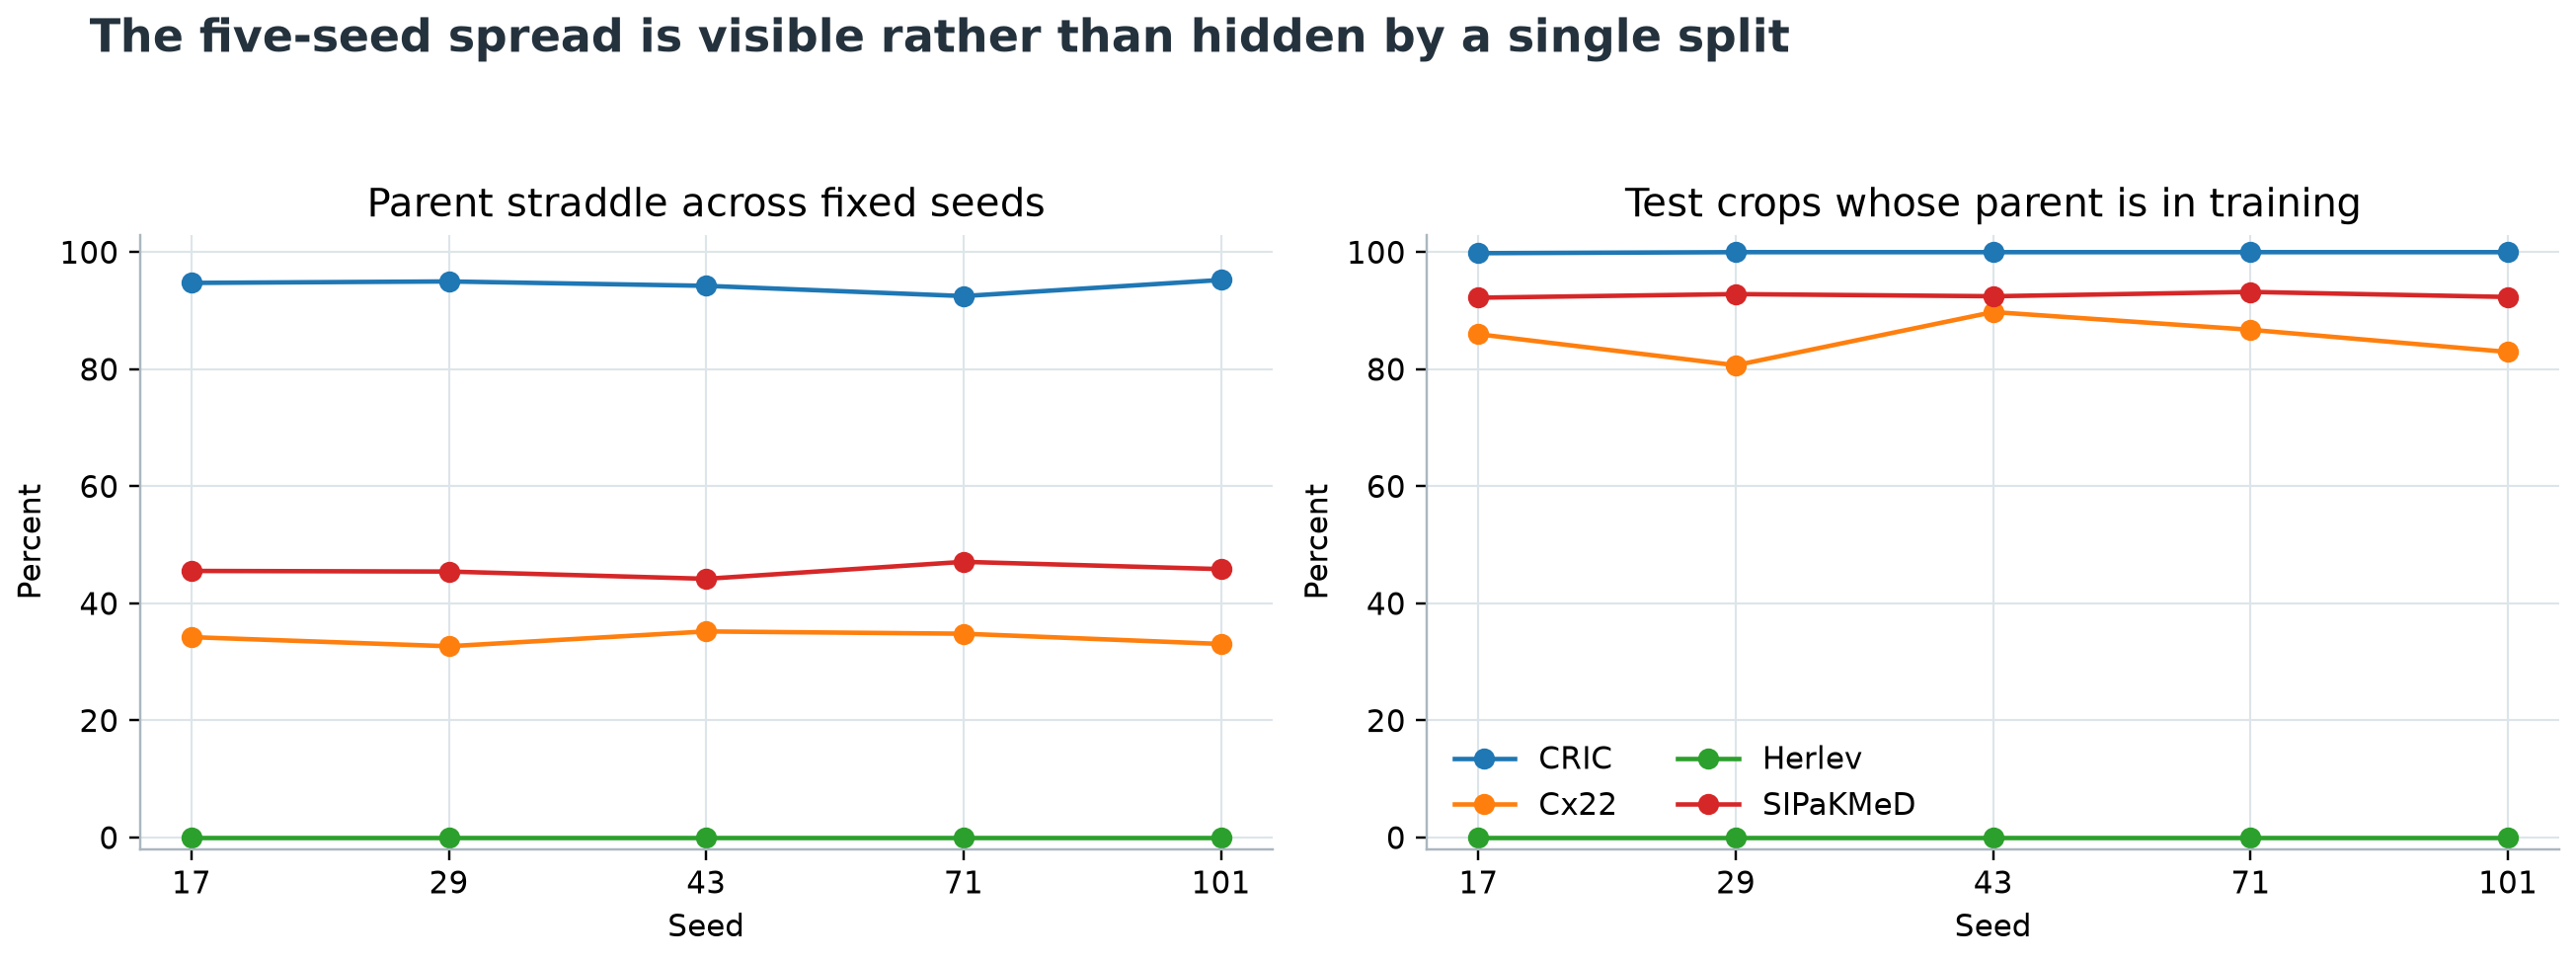
\includegraphics[width=\textwidth]{structural_seed_spread.png}
\caption{Seed-level structural results. Reporting the spread prevents one convenient split from defining the claim.}
\label{fig:structural-seeds}
\end{figure}

\section{Interpretation}

CRIC is the most extreme because its parents emit 28.84 crops on average: essentially every random-split test cell has a source image in training. SIPaKMeD and Cx22 have lower parent multiplicity, yet 92.62\% and 85.23\% of their test observations respectively still have a training sibling. Herlev establishes implementation specificity: the same code returns zero when the data genuinely have one observation per parent.

The structural ordering P3 $\leq$ P2 $\leq$ P1 passes for all datasets. This statement concerns shared parents, not model scores. Later, the analogous model-score ordering fails for four of six SIPaKMeD classifiers; the two outcomes are logically compatible.

\chapter{Literal overlap and conservative duplicate grouping}

\section{Literal source-pixel overlap}

SIPaKMeD's recovered boxes permit a stronger question than shared parent identity. Let boxes $B_i$ and $B_j$ come from the same field. Their intersection is non-empty when
\begin{equation}
\max(x_i,x_j)<\min(x_i+w_i,x_j+w_j)
\quad\text{and}\quad
\max(y_i,y_j)<\min(y_i+h_i,y_j+h_j).
\end{equation}
The intersection-over-union is
\begin{equation}
\operatorname{IoU}(B_i,B_j)=\frac{|B_i\cap B_j|}{|B_i\cup B_j|}.
\end{equation}

Across 13,064 within-parent crop pairs, 2,185 share at least one pixel and the maximum IoU is 0.546. Under P1, 16.80$\pm$0.77\% of cross-split sibling pairs overlap and 52.62$\pm$1.97\% of test crops overlap at least one source pixel with a training crop. Both quantities are 0.00$\pm$0.00\% under P2 and P3.

\begin{figure}[H]
\centering
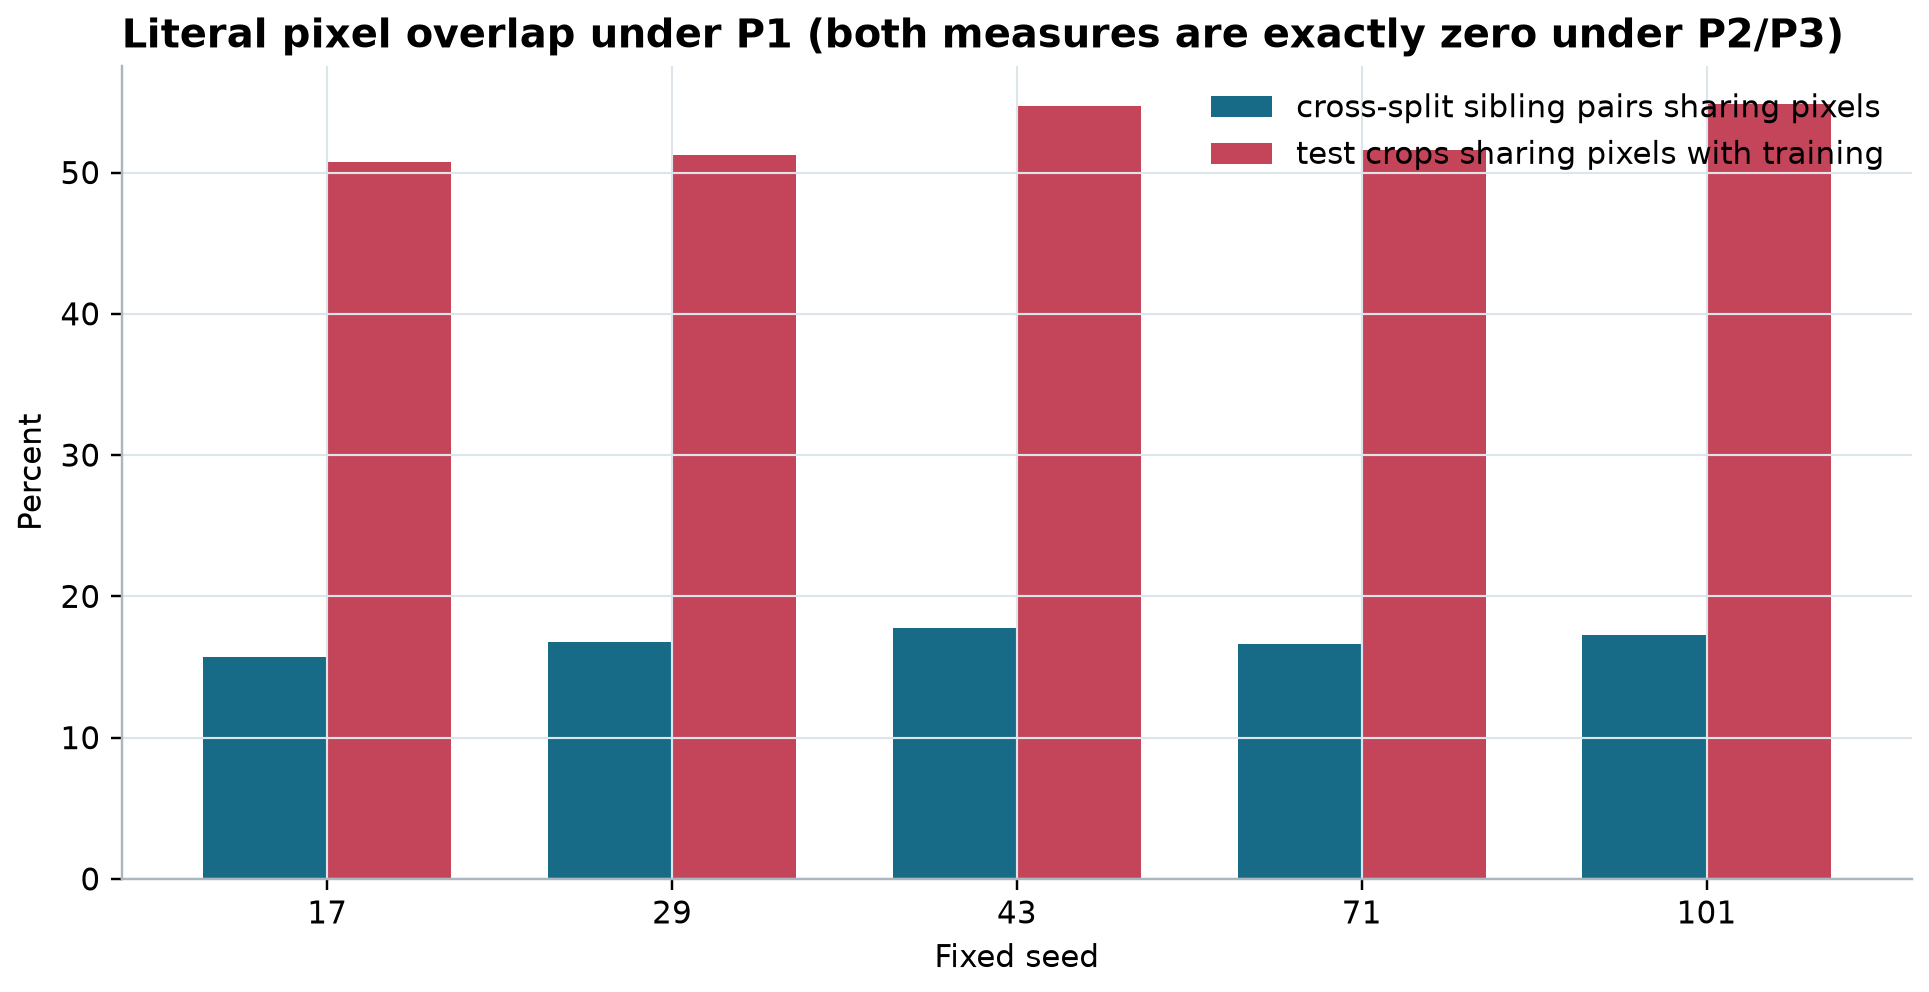
\includegraphics[width=0.9\textwidth]{literal_pixel_overlap.png}
\caption{Literal overlap for every P1 seed. The larger test-crop fraction answers a different question from the pair fraction: whether each test crop has at least one overlapping training sibling.}
\label{fig:pixel-overlap}
\end{figure}

\section{Perceptual hashes and P3}

For each crop the implementation computes a 64-bit perceptual hash from the median-thresholded low-frequency $8\times8$ DCT block and a 64-bit difference hash from adjacent comparisons in an $8\times9$ downsample. Two crops become a candidate pair when they are pixel-exact or when both Hamming distances are at most six. Cross-parent candidate pairs are joined by union-find; each connected component becomes one P3 group.

At the frozen thresholds, the audit found 201 cross-parent candidate pairs. They connect 170 parent IDs into 74 components, the largest containing eight parents, and reduce 966 parents to 870 P3 groups. No pair is pixel-exact. A synthetic calibration detected all three injected transformations and rejected all 100 deterministic unrelated-parent negatives, yielding precision 1.00 and recall 1.00 on that calibration set.

\begin{figure}[H]
\centering
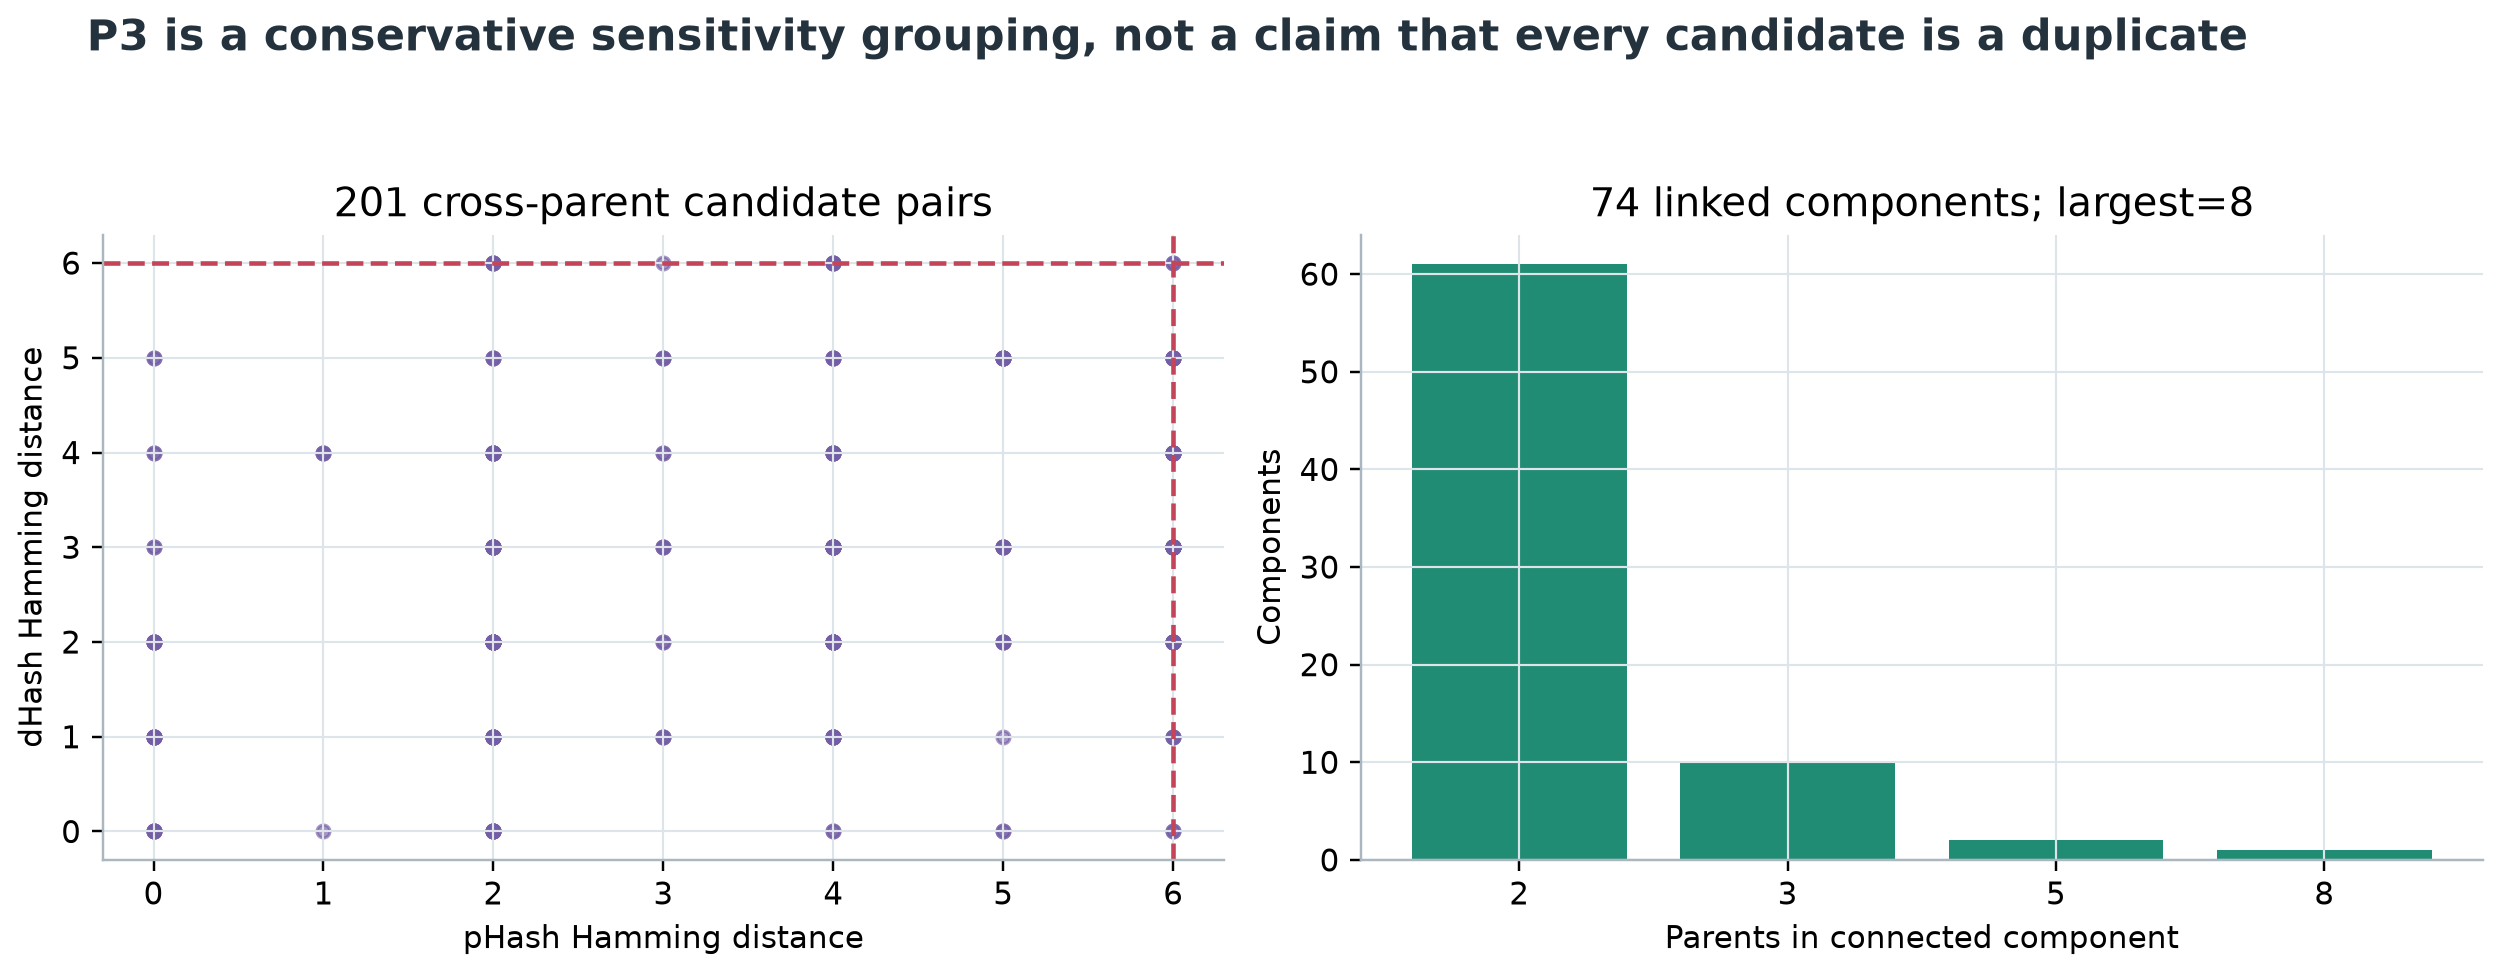
\includegraphics[width=\textwidth]{duplicate_audit.png}
\caption{Near-duplicate sensitivity audit. The thresholded candidates are used conservatively for grouping; they are not treated as ground-truth duplicate annotations.}
\label{fig:duplicates}
\end{figure}

\begin{warningbox}{What the duplicate experiment did not do}
The broader planning idea mentioned a three-detector majority vote involving learned features. The frozen release implements only the pHash+dHash consensus audit and its synthetic calibration. Therefore the report does not claim a CNN/domain-encoder duplicate ensemble, human-confirmed duplicate truth, or general detector precision outside the calibration set.
\end{warningbox}

\chapter{The parent-identity mechanism probe}

\section{Motivation}

Structural overlap says that siblings are present. The parent probe asks whether their shared source is visually recoverable after cellular content and color cues are altered. A positive answer makes the shortcut concrete: a learner can recognize the parent field from a different crop. It still does not prove that a morphology classifier uses that signal.

\section{Balanced task construction}

Parents with at least four crops are eligible. The minimum eligible size allows two training and two test crops per parent. To make chance exact, each eligible parent contributes the same number of training and test crops. The final task contains 424 parents, 848 training crops, and 848 test crops, so chance is
\begin{equation}
P_{\mathrm{chance}}=\frac{1}{424}=0.00235849=0.235849\%.
\end{equation}

A ResNet-18~\cite{he2016resnet} initialized from ImageNet replaces its final layer with a 424-way linear classifier. It trains for 15 epochs with AdamW~\cite{loshchilov2019adamw}, learning rate $10^{-4}$, weight decay $10^{-4}$, batch size 64, and fixed seeds. Training augmentation is a random resized crop with scale 0.85--1.0 plus horizontal and vertical flips; testing resizes to $224\times224$. ImageNet normalization follows every image-mode transform.

\section{Image transformations and their motivations}

\subsection{RGB}
RGB is the maximal-information condition. It permits morphology, stain, illumination, background, focus, acquisition artifacts, and any other visible cue.

\subsection{Grayscale}
Grayscale removes hue and saturation while retaining luminance, edges, morphology, focus, and texture. Persistence here means identity is not solely a stain-color phenomenon.

\subsection{LAB stain normalization}
RGB is converted to CIE LAB. For channel vector $z$, source mean $\mu_s$, source standard deviation $\sigma_s$, and fixed target statistics $\mu_t=(190,140,135)$ and $\sigma_t=(35,14,14)$, the implemented transform is
\begin{equation}
z'=\operatorname{clip}\left((z-\mu_s)\odot\frac{\sigma_t}{\max(\sigma_s,1)}+\mu_t,0,255\right).
\end{equation}
This is a fixed-statistics color-transfer normalization based on the logic of Reinhard et al.~\cite{reinhard2001color}. Persistence means simple first- and second-moment color normalization does not erase the source fingerprint.

\subsection{Background-only: Otsu, morphology, and Telea inpainting}

This condition deliberately removes the likely cell foreground. The implementation converts RGB to HSV and grayscale, then independently obtains Otsu thresholds~\cite{otsu1979threshold} on saturation $S$ and luminance $Y$. The preliminary foreground mask is
\begin{equation}
M_0(u)=\mathbf{1}\{S(u)>t_S\;\lor\;Y(u)<t_Y\}.
\end{equation}
A $5\times5$ morphological closing fills small holes and connects narrow gaps:
\begin{equation}
M=(M_0\oplus K)\ominus K.
\end{equation}
Finally, the marked region is filled from its boundary with Telea's fast-marching inpainting method using radius 5~\cite{telea2004inpainting}. The result keeps background statistics while suppressing the cell body and nucleus. A successful classifier in this condition shows that background alone carries considerable parent information.

\subsection{High-pass}
For Gaussian blur $G_{\sigma=3}*I$, the residual is
\begin{equation}
I_{\mathrm{hp}}=\operatorname{clip}\left(I-G_{\sigma=3}*I+128,0,255\right).
\end{equation}
This suppresses low-frequency illumination and emphasizes local texture, edges, compression, and focus structure.

\begin{figure}[H]
\centering
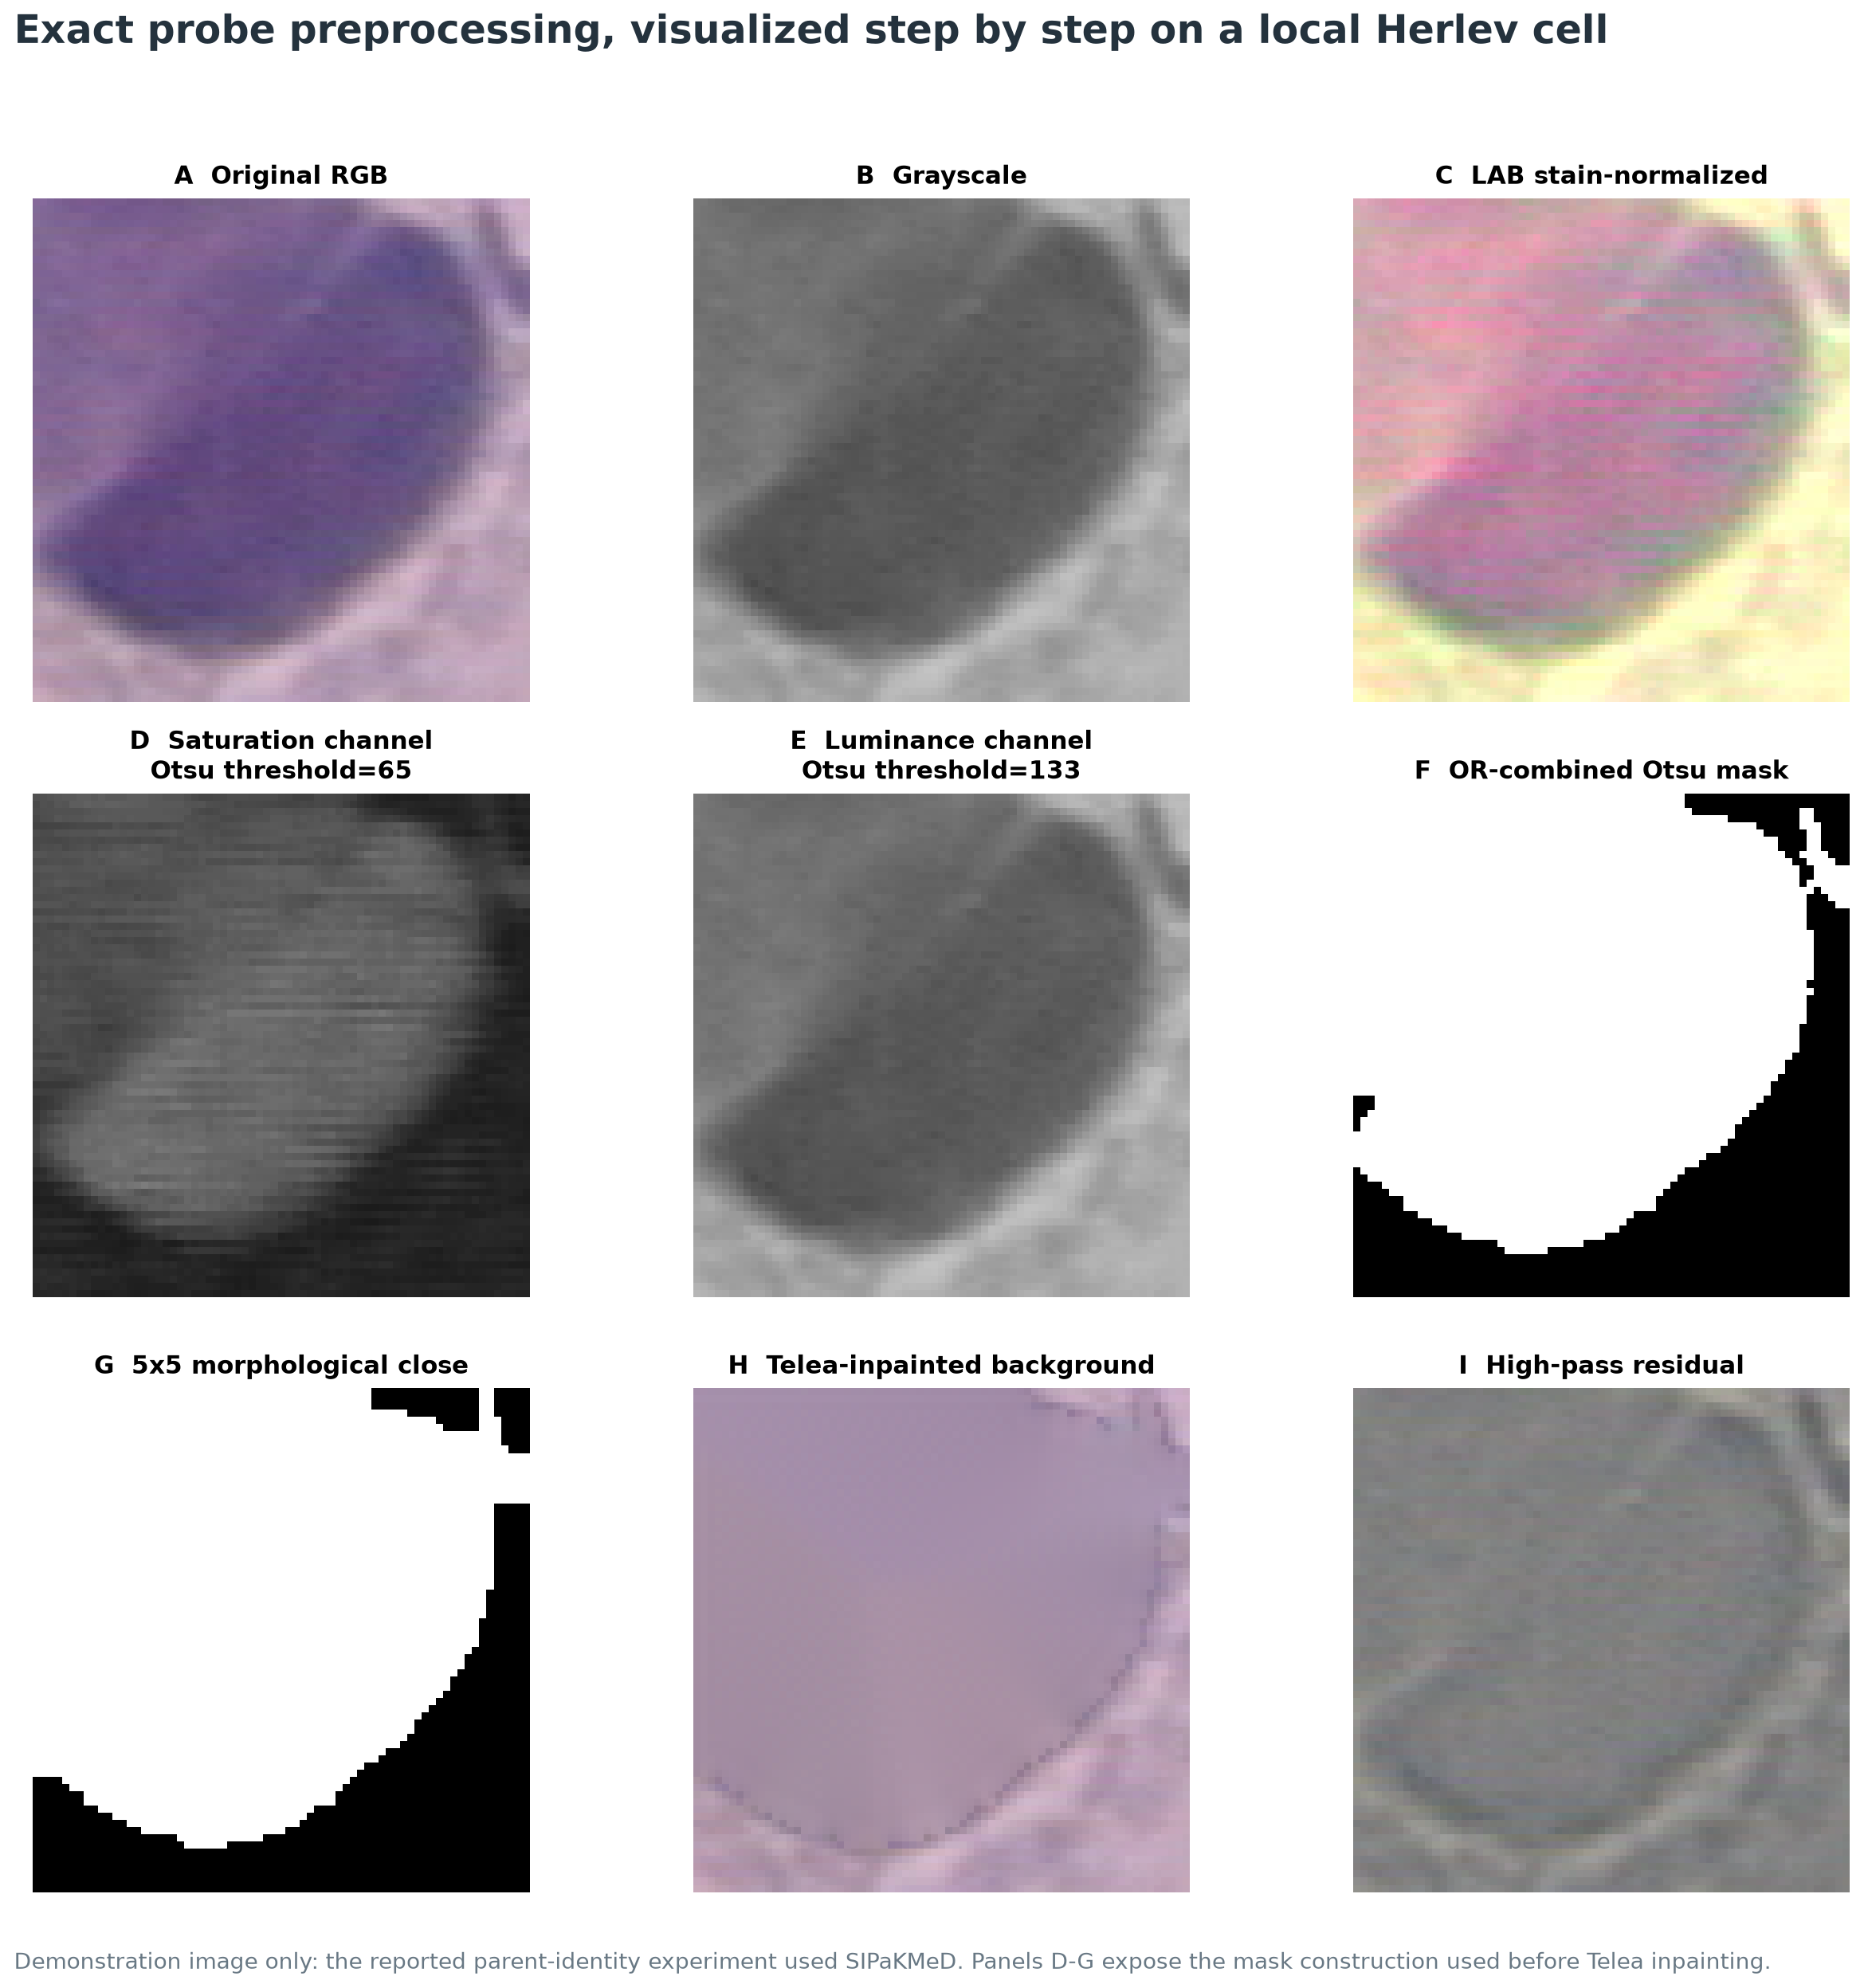
\includegraphics[width=0.92\textwidth]{probe_transformations.png}
\caption{Every preprocessing stage shown on an actual local Herlev cell. This is an implementation demonstration, not a probe result image: the reported parent-identification experiment used SIPaKMeD crops. Panels D--G make Otsu thresholding, mask combination, and morphological closing visible before Telea inpainting.}
\label{fig:transformations}
\end{figure}

\section{Shuffled-label negative control}

Only the training labels are permuted, using the same images, optimizer, epochs, seeds, and task size. The five-seed 95\% interval must cover the exact chance baseline. Otherwise the probe would be rejected because a bookkeeping or imbalance artifact could explain apparent identity learning.

\section{Results}

\begin{table}[H]
\centering
\caption{Parent-identity probe. Mean $\pm$ sample SD over five seeds.}
\label{tab:probe}
\begin{tabular}{lrr}
\toprule
Input condition & Accuracy & Multiple of chance \\
\midrule
RGB & 25.73$\pm$0.66\% & 109.1$\times$ \\
Grayscale & 13.80$\pm$1.12\% & 58.5$\times$ \\
Stain-normalized & 17.31$\pm$0.64\% & 73.4$\times$ \\
Background-only & 18.68$\pm$1.25\% & 79.2$\times$ \\
High-pass & 16.27$\pm$0.60\% & 69.0$\times$ \\
Shuffled RGB labels & 0.17$\pm$0.24\% & 0.7$\times$ \\
\bottomrule
\end{tabular}
\end{table}

\begin{figure}[H]
\centering
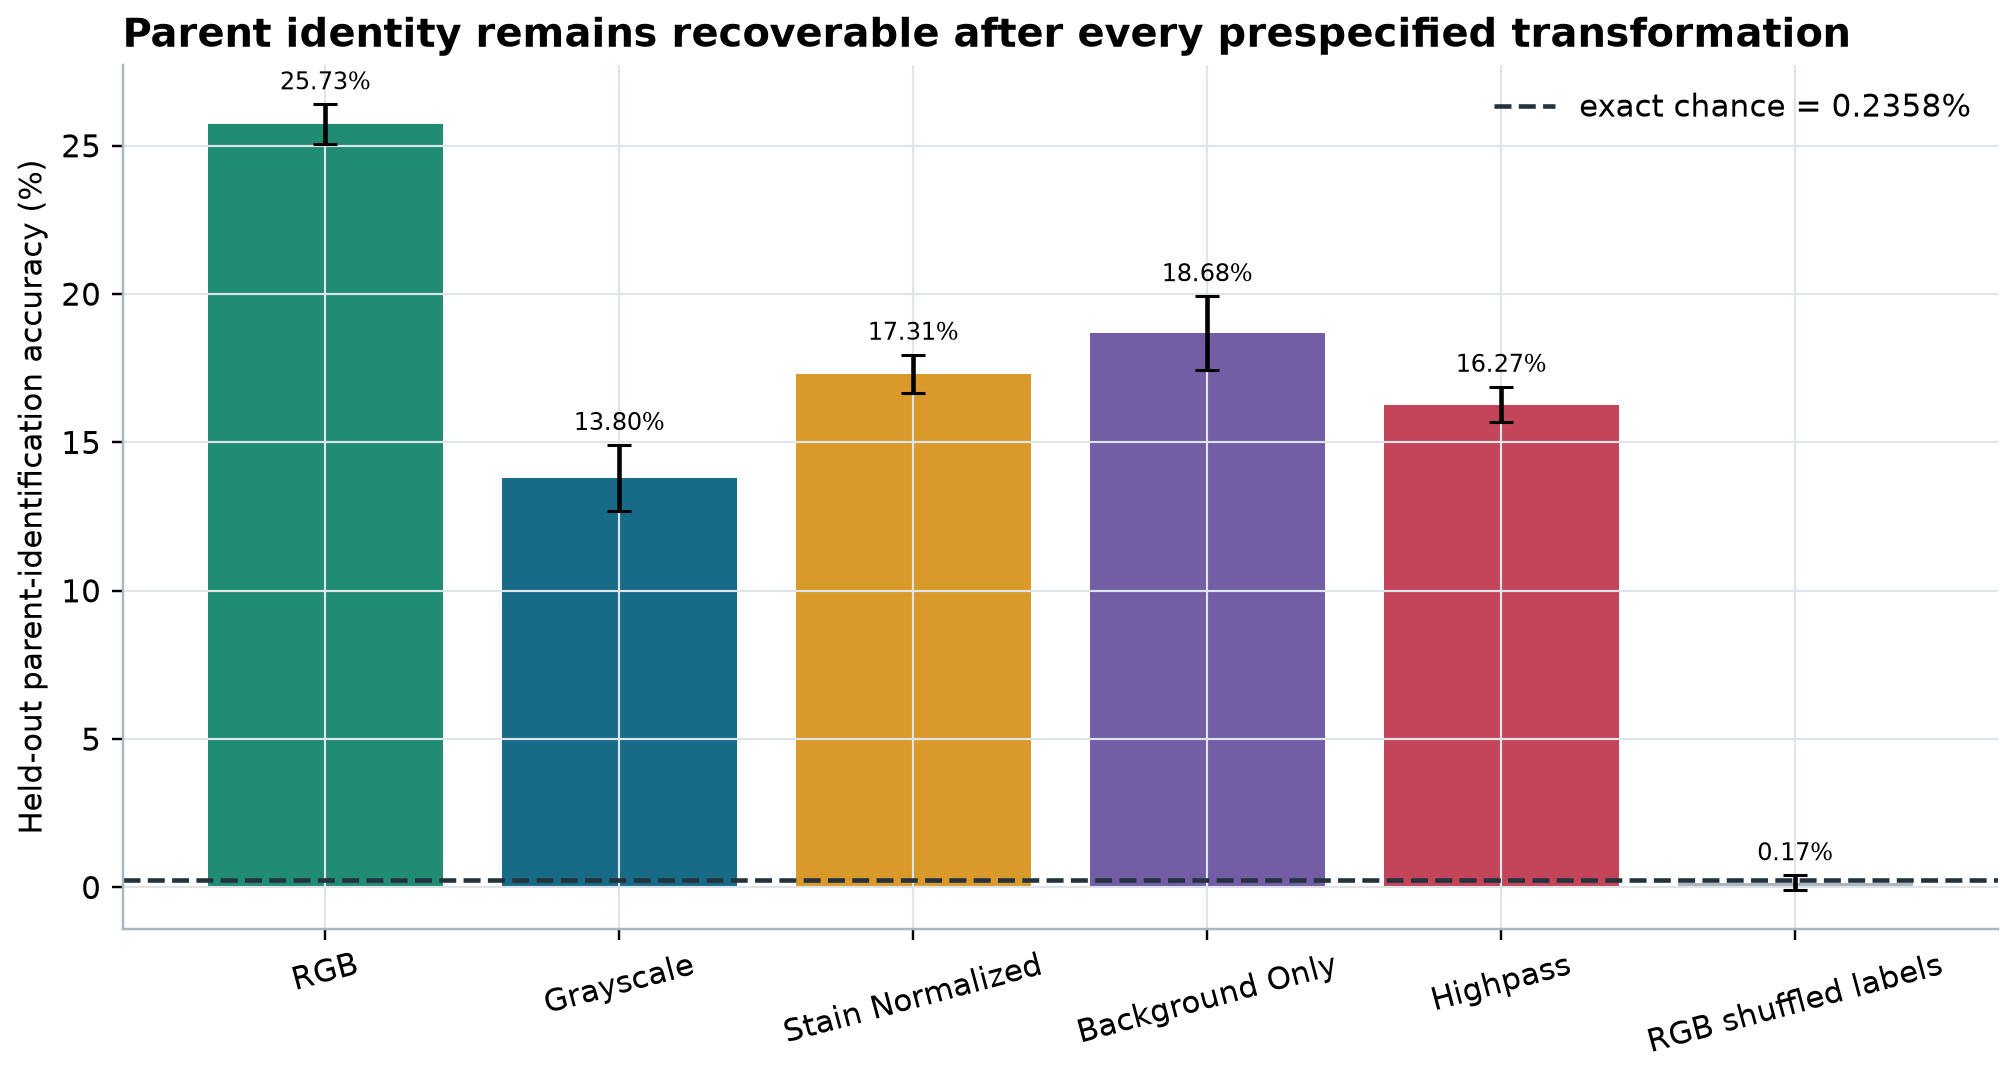
\includegraphics[width=0.92\textwidth]{probe_results.png}
\caption{All prespecified image conditions remain far above chance. Error bars are sample SD across five seeds.}
\label{fig:probe-results}
\end{figure}

\begin{figure}[H]
\centering
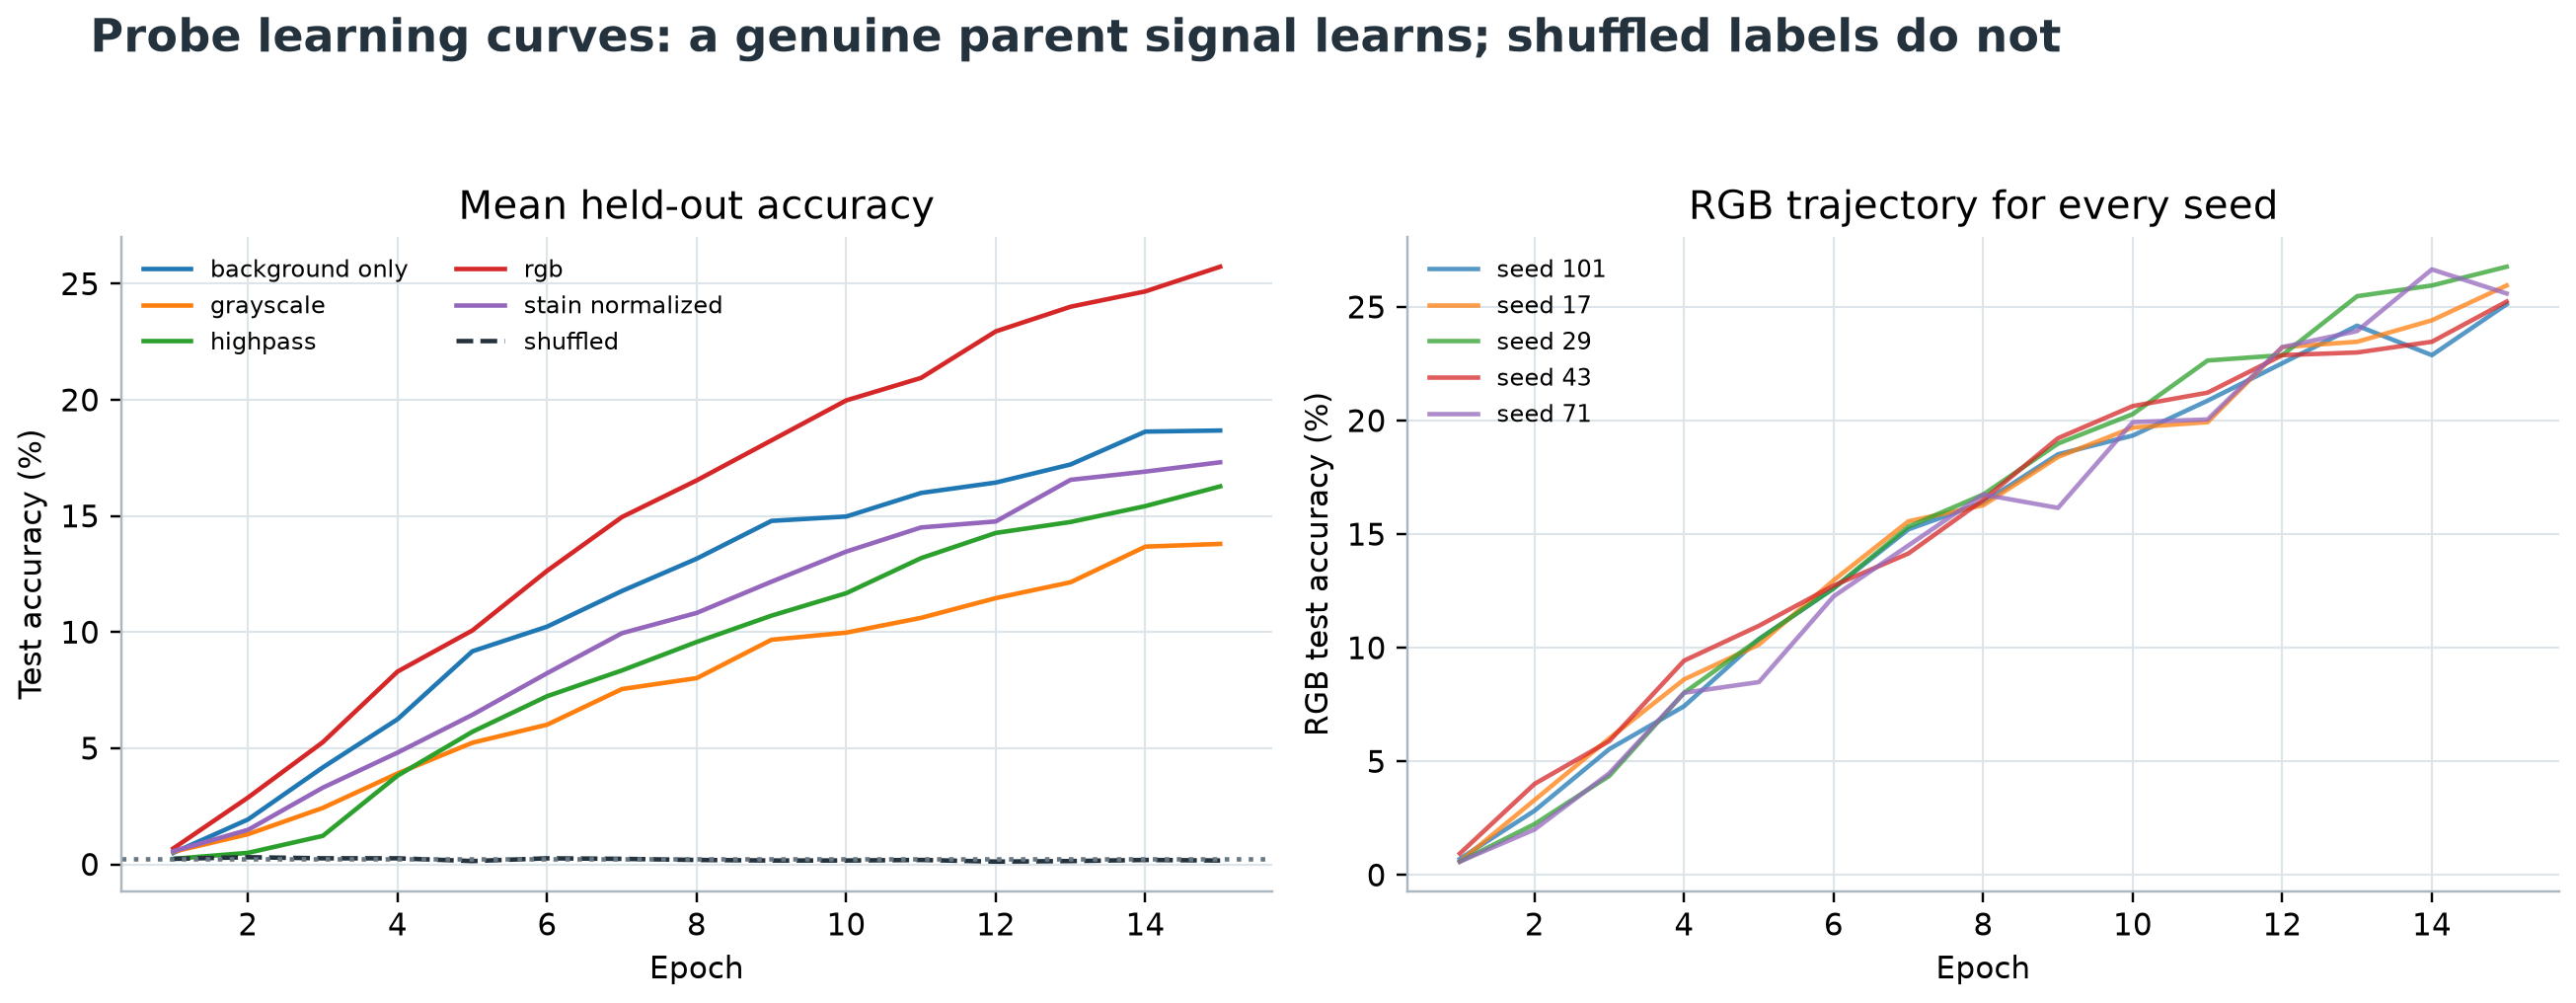
\includegraphics[width=\textwidth]{probe_learning_curves.png}
\caption{Probe learning curves reconstructed from every retained epoch history. The RGB signal rises smoothly across seeds; shuffled labels remain near chance.}
\label{fig:probe-learning}
\end{figure}

The shuffled mean is 0.1651\%, SD 0.2445 percentage points, with a five-seed interval from $-0.1385$\% to 0.4687\%; the exact 0.2358\% chance value lies inside. A negative lower confidence limit is an ordinary symmetric small-sample interval artifact and does not imply negative accuracy.

Background-only accuracy is higher than grayscale and stain-normalized accuracy. That does not mean background is the only cue: RGB remains highest, and transformations alter multiple image properties at once. The careful conclusion is that parent information is distributed across color, low- and high-frequency structure, and background.

\chapter{SIPaKMeD classification rescore}

\section{Why re-run models rather than quote published scores?}

Published numbers are entangled with architectures, preprocessing, augmentations, and---most importantly---different splits. Quoting them would not isolate the quantity of interest. The rescore therefore trains six representative image classifiers under the same code path, preprocessing, optimizer family, epoch budget, seeds, and four fixed split protocols. The only intended change across protocols is the independence constraint and, for the explicitly size-matched control, the number of retained training crops.

The six families cover different inductive biases and capacities: ResNet-18 and ResNet-50~\cite{he2016resnet}, DenseNet-121~\cite{huang2017densenet}, MobileNet-V2~\cite{sandler2018mobilenetv2}, EfficientNet-B0~\cite{tan2019efficientnet}, and ViT-B/16~\cite{dosovitskiy2021vit}. Each ImageNet-pretrained head is replaced with a five-way linear classifier. Re-running all six also prevents the conclusion from depending on one especially favorable architecture.

\section{Inputs, augmentation, and optimization}

Every crop is decoded as RGB, converted to a tensor, and normalized by the ImageNet channel statistics. Training augmentation consists of a random resized crop to $224\times224$ with scale in $[0.8,1.0]$, a horizontal flip, and a vertical flip. Test preprocessing is a deterministic resize to $224\times224$. The code records the fully resolved split hash and configuration beside every result.

All classifiers use AdamW~\cite{loshchilov2019adamw}, cross-entropy loss, and a fixed learning rate. The retained endpoint is the final epoch; there is no separate validation split or post-hoc best-epoch selection. A run is valid only when the stored identifiers match its split, the final file is complete, and all reported quantities are finite. Table~\ref{tab:classifier-hparams} gives the execution contract.

\begin{table}[H]
\centering
\caption{SIPaKMeD classifier execution settings.}
\label{tab:classifier-hparams}
\begin{tabular}{ll}
\toprule
Item & Setting \\
\midrule
Architectures & ResNet-18/50, DenseNet-121, MobileNet-V2, EfficientNet-B0, ViT-B/16 \\
Initialization & ImageNet pretrained \\
Input & RGB, $224\times224$ \\
Loss & Five-class cross entropy \\
Optimizer & AdamW \\
Learning rate & $10^{-4}$, fixed \\
Weight decay & $10^{-4}$ \\
Batch size & 64 \\
Epochs & 20, final-epoch endpoint \\
Seeds & 17, 29, 43, 71, 101 \\
Primary metric & Test accuracy \\
Hardware & NVIDIA RTX A6000; at most three concurrent GPU jobs \\
\bottomrule
\end{tabular}
\end{table}

\section{Metric definitions}

For true class $y_i$ and prediction $\hat y_i$, accuracy is
\begin{equation}
\operatorname{Acc}=\frac{1}{N}\sum_{i=1}^{N}\mathbf{1}\{\hat y_i=y_i\}.
\end{equation}
For class $c$, with precision $P_c$ and recall $R_c$,
\begin{equation}
F_{1,c}=\frac{2P_cR_c}{P_c+R_c},\qquad
F_{1,\mathrm{macro}}=\frac{1}{C}\sum_{c=1}^{C}F_{1,c}.
\end{equation}
Balanced accuracy is the unweighted mean class recall,
\begin{equation}
\operatorname{BAcc}=\frac{1}{C}\sum_{c=1}^{C}\frac{TP_c}{TP_c+FN_c}.
\end{equation}
The preregistered primary endpoint is accuracy. Macro-F1 and balanced accuracy check that the direction is not a class-frequency artifact; they are not used to shop for a smaller $p$-value.

\section{Aggregate scores}

\begin{table}[H]
\centering
\caption{SIPaKMeD test accuracy (\%), mean $\pm$ sample SD over five seeds. \protocol{P1$'$} is numerically identical to \protocol{P1} because the frozen stratified crop split already contained the registered 3,239 training and 810 test observations.}
\label{tab:classification-main}
\small
\begin{tabular}{lrrrr}
\toprule
Architecture & \protocol{P1} & \protocol{P1$'$} & \protocol{P2} & \protocol{P3} \\
\midrule
DenseNet-121 & 98.12$\pm$0.28 & 98.12$\pm$0.28 & 96.72$\pm$0.69 & 97.38$\pm$0.50 \\
EfficientNet-B0 & 97.78$\pm$0.49 & 97.78$\pm$0.49 & 96.69$\pm$1.49 & 97.41$\pm$0.71 \\
MobileNet-V2 & 97.41$\pm$0.45 & 97.41$\pm$0.45 & 95.16$\pm$1.50 & 96.20$\pm$0.93 \\
ResNet-18 & 97.19$\pm$0.59 & 97.19$\pm$0.59 & 96.00$\pm$0.89 & 96.35$\pm$1.28 \\
ResNet-50 & 97.51$\pm$0.47 & 97.51$\pm$0.47 & 96.79$\pm$0.42 & 96.27$\pm$0.53 \\
ViT-B/16 & 97.14$\pm$0.95 & 97.14$\pm$0.95 & 95.56$\pm$0.84 & 95.53$\pm$1.68 \\
\bottomrule
\end{tabular}
\end{table}

\begin{figure}[H]
\centering
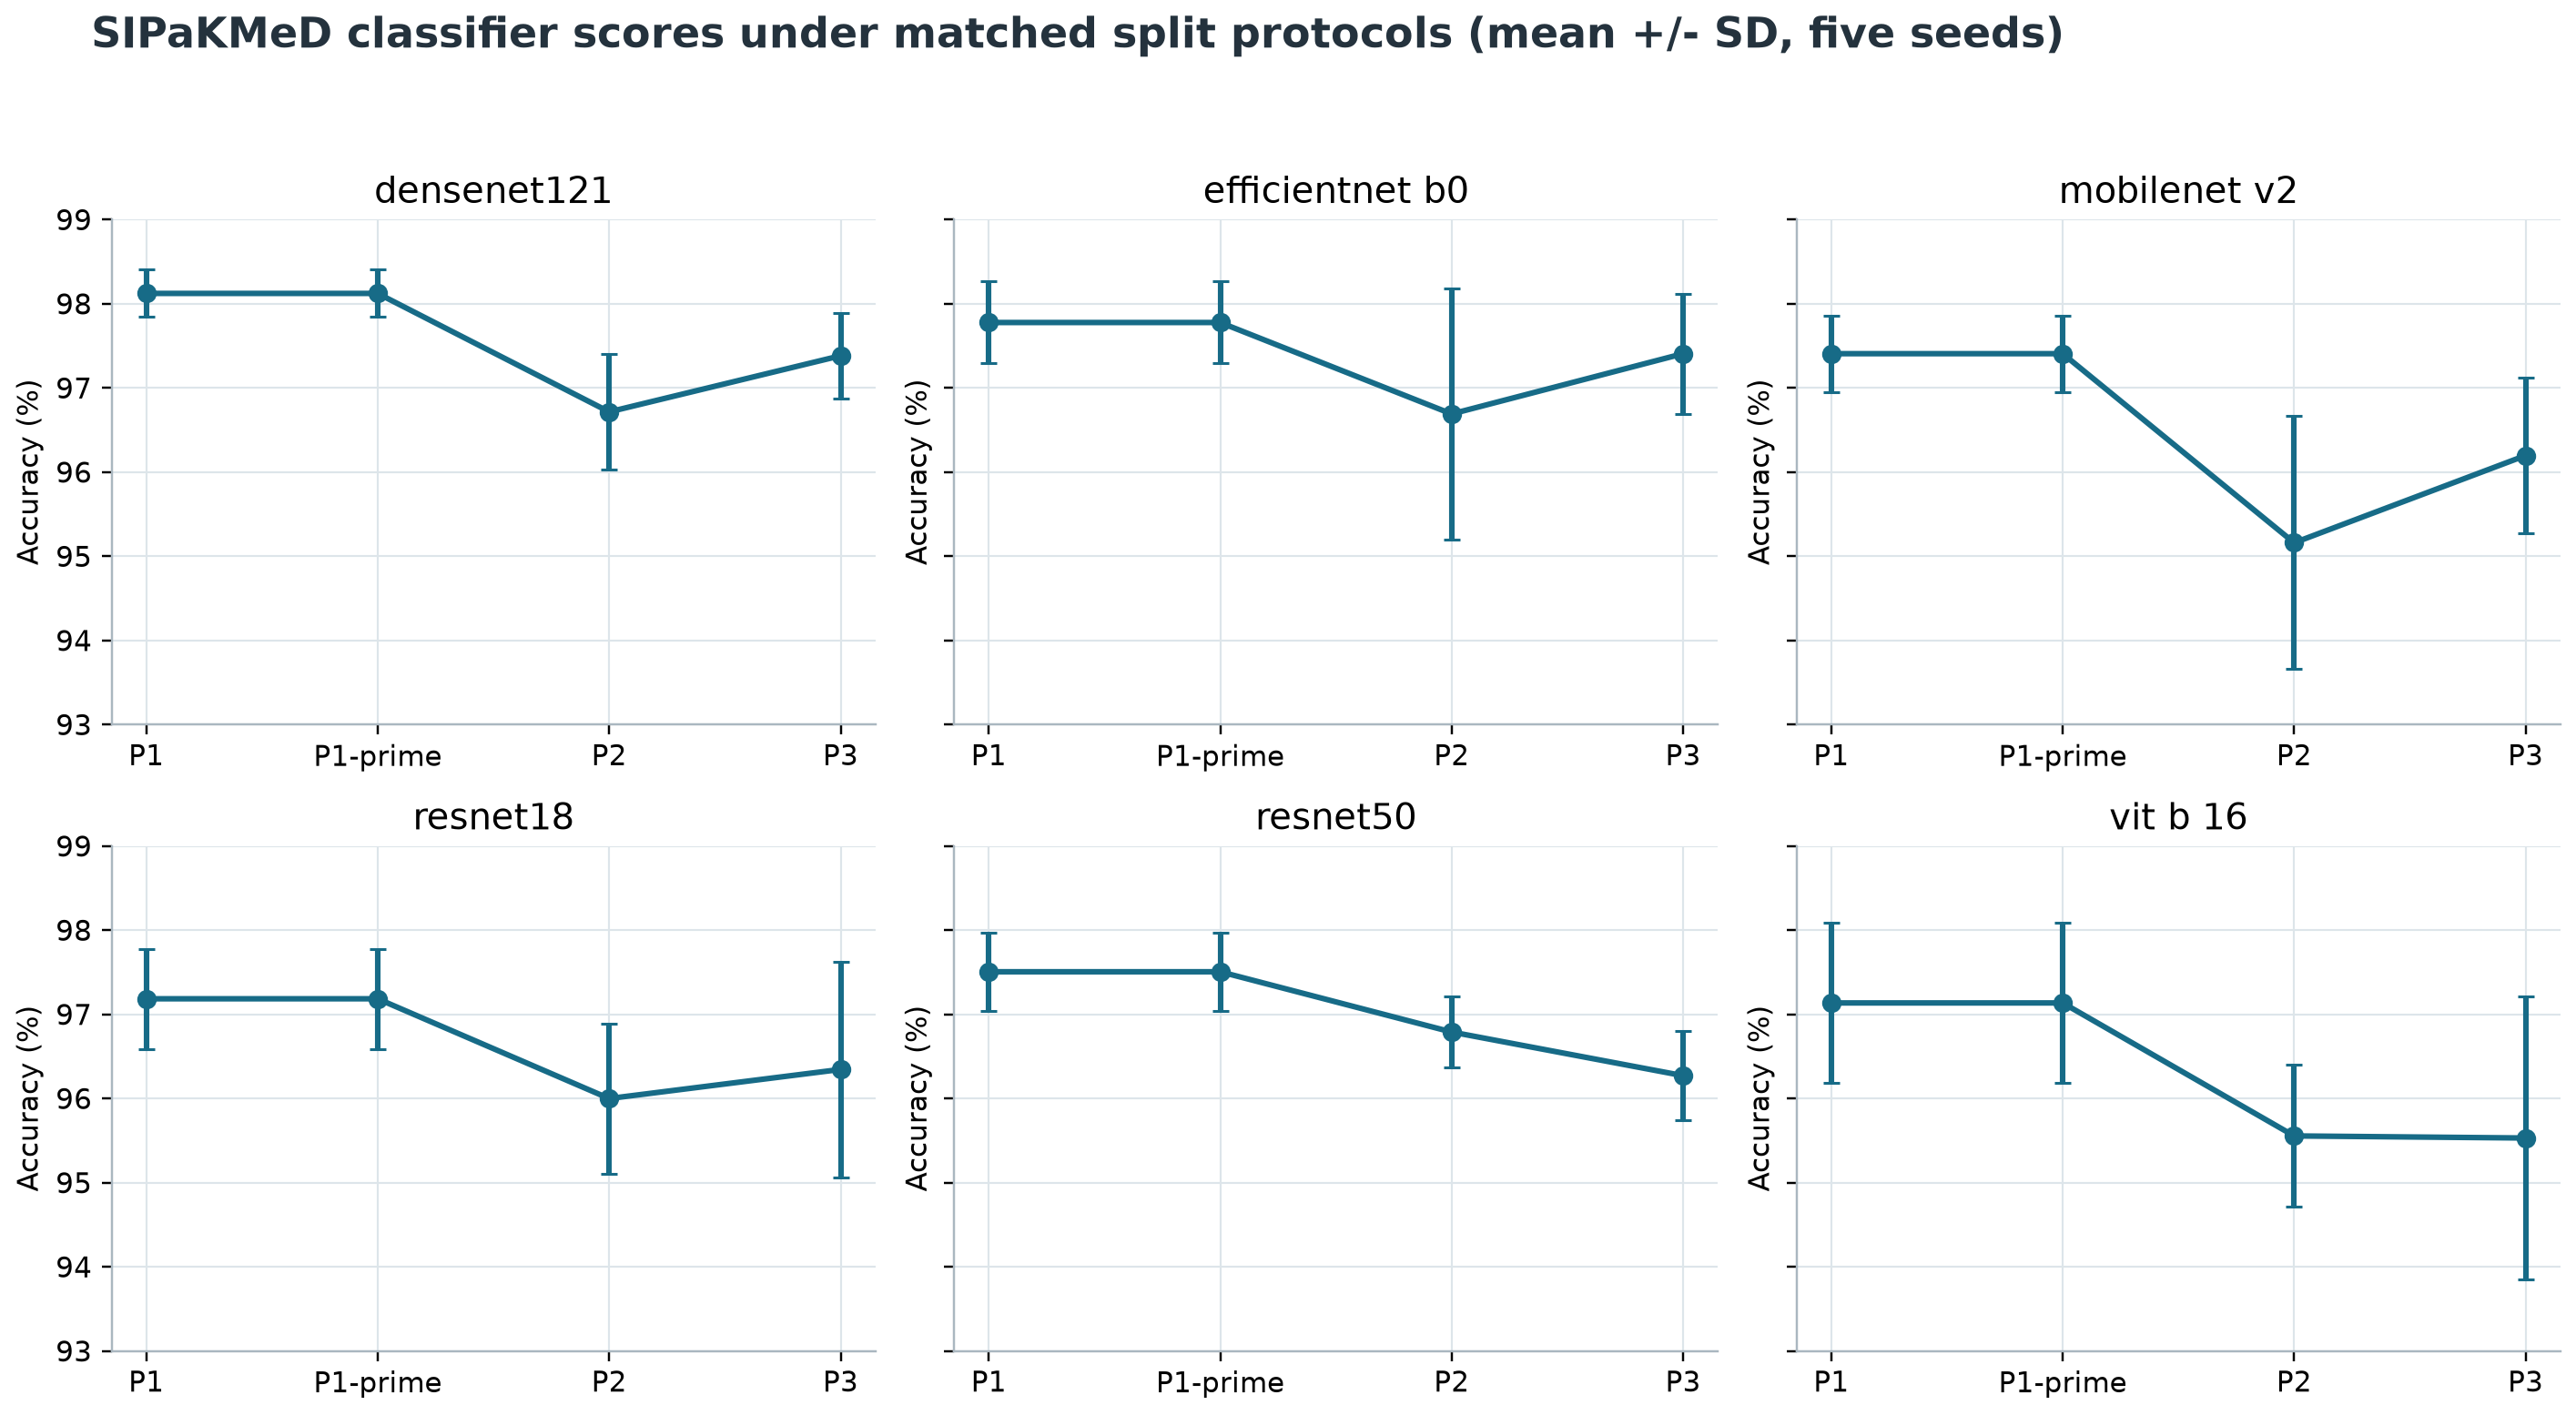
\includegraphics[width=\textwidth]{classification_protocol_scores.png}
\caption{All frozen SIPaKMeD accuracy observations. Lines connect the same architecture across protocols; points show individual seeds and bars show the mean.}
\label{fig:classification-scores}
\end{figure}

The top score under \protocol{P1} is DenseNet-121 at 98.12$\pm$0.28\%. Under parent-disjoint \protocol{P2}, DenseNet-121 remains highest at 96.72$\pm$0.69\%, narrowly followed by ResNet-50. The key scientific observation is not which backbone wins; it is that all six paired \protocol{P1}$-$\protocol{P2} mean differences are positive.

\section{Matched contrasts, uncertainty, and the ordering failure}

For architecture $a$ and seed $s$, the primary paired difference is
\begin{equation}
d_{a,s}=100\left(\operatorname{Acc}_{a,s,\mathrm{P1}}-
\operatorname{Acc}_{a,s,\mathrm{P2}}\right)
\end{equation}
in percentage points. The paired standardized effect is Cohen's
\begin{equation}
d_z=\frac{\bar d}{s_d},
\end{equation}
where $s_d$ is the sample SD of the five seed-paired differences. Reported effect-size confidence intervals are seed-paired bootstrap intervals, so a bootstrap resample always keeps the two protocol results from a seed together. The test is a paired $t$-test because every registered five-difference vector passed its Shapiro--Wilk screen; the switch to Wilcoxon was reserved for a failed screen.

\begin{table}[H]
\centering
\caption{Primary SIPaKMeD \protocol{P1}$-$\protocol{P2} contrasts. The six paired $t$-tests form one preregistered BH family. CI is the paired-bootstrap 95\% interval for Cohen's $d_z$, not for the raw percentage-point mean.}
\label{tab:classification-contrasts}
\small
\begin{tabular}{lrrrrr}
\toprule
Architecture & Mean$\pm$SD (pp) & 95\% CI for $d_z$ & $p$ & BH $q$ & $d_z$ \\
\midrule
DenseNet-121 & 1.41$\pm$0.90 & [0.985, 4.747] & 0.0251 & 0.1109 & 1.561 \\
EfficientNet-B0 & 1.09$\pm$1.85 & [$-$0.316, 4.668] & 0.2591 & 0.2591 & 0.588 \\
MobileNet-V2 & 2.25$\pm$1.63 & [0.809, 6.686] & 0.0370 & 0.1109 & 1.377 \\
ResNet-18 & 1.19$\pm$1.28 & [0.442, 2.365] & 0.1081 & 0.1511 & 0.922 \\
ResNet-50 & 0.72$\pm$0.83 & [0.085, 4.025] & 0.1260 & 0.1511 & 0.863 \\
ViT-B/16 & 1.58$\pm$1.70 & [0.057, 4.950] & 0.1059 & 0.1511 & 0.931 \\
\bottomrule
\end{tabular}
\end{table}

\begin{figure}[H]
\centering
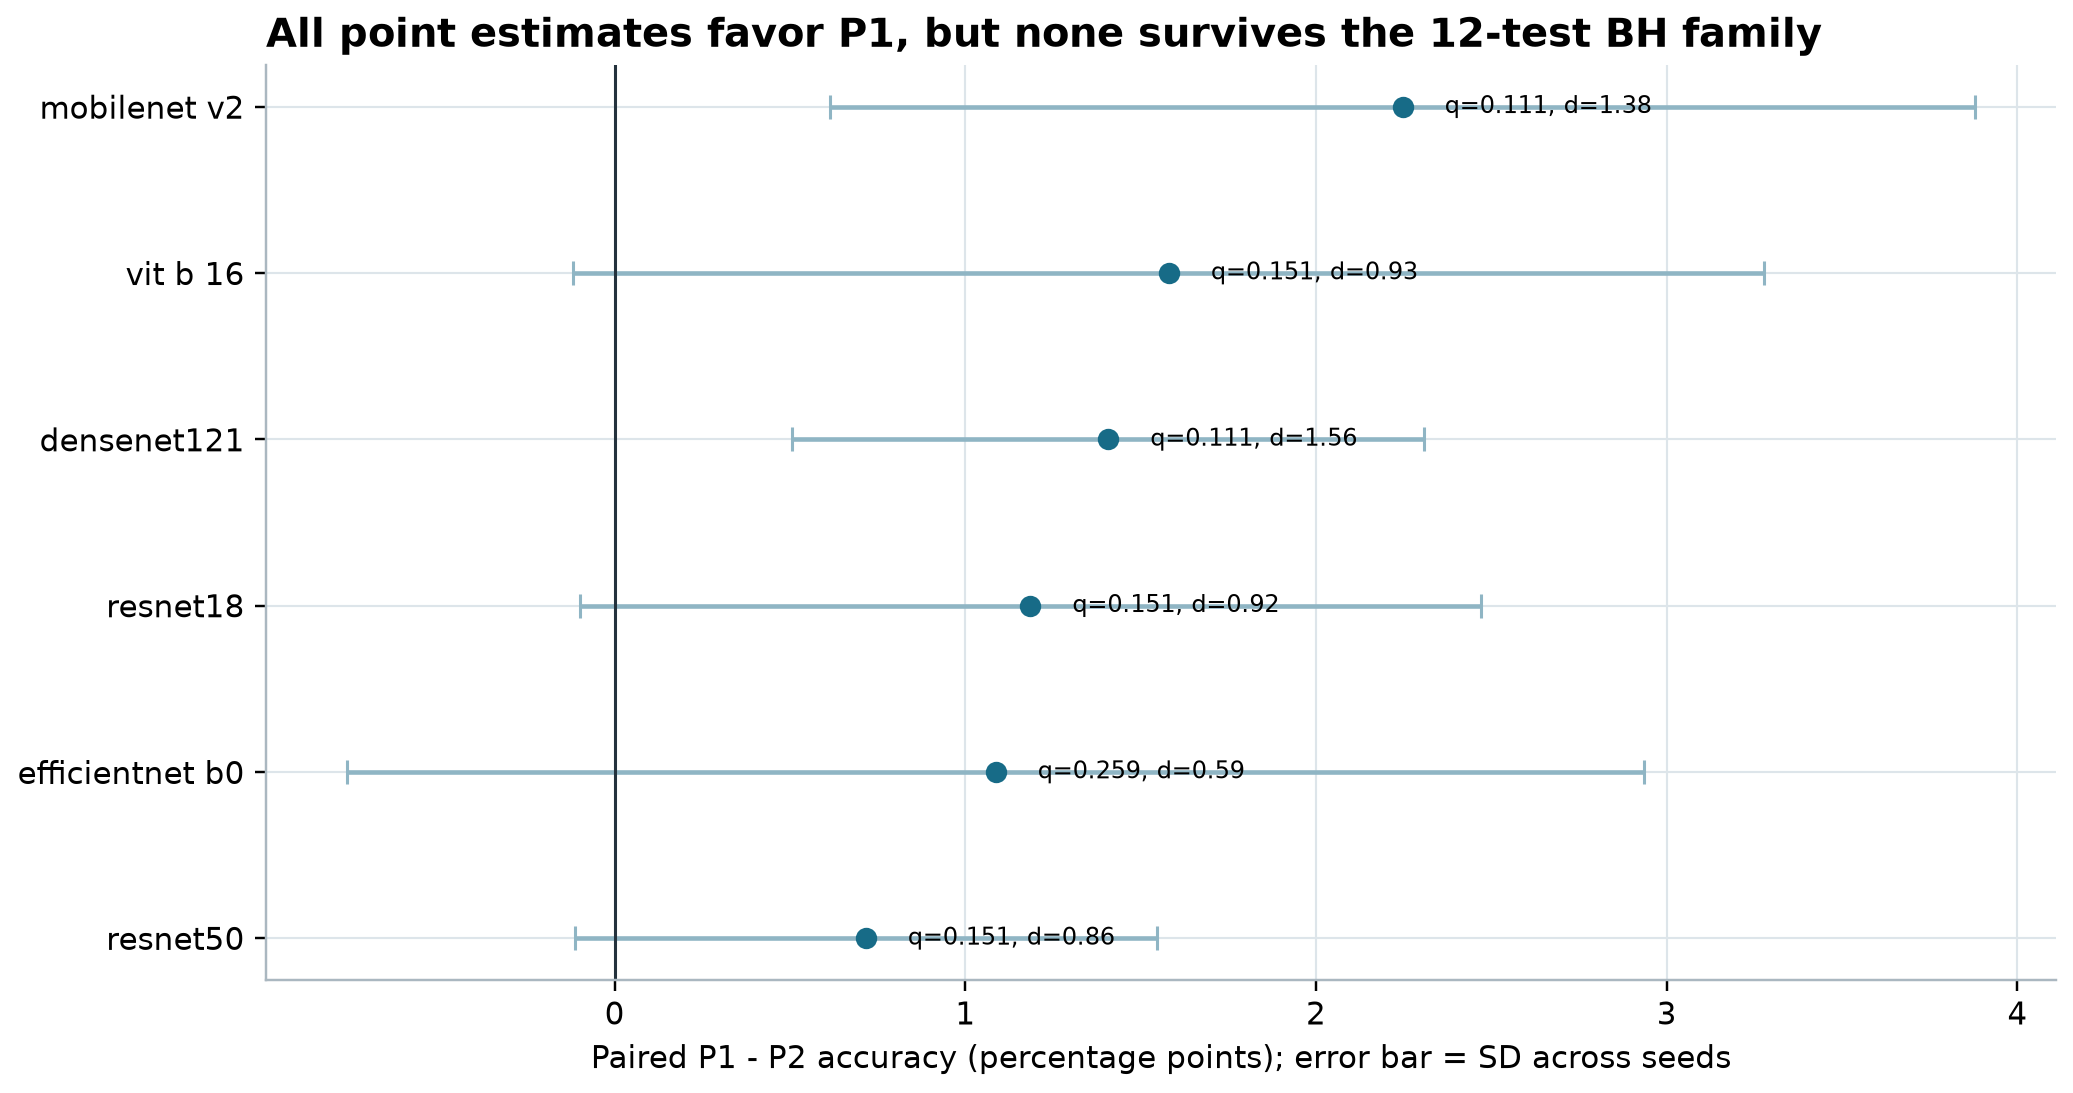
\includegraphics[width=\textwidth]{classification_delta_forest.png}
\caption{Paired \protocol{P1}$-$\protocol{P2} effects. Every mean favors the crop-level split, but none survives its preregistered multiplicity correction. The vertical line at zero marks no protocol effect.}
\label{fig:classification-forest}
\end{figure}

\begin{figure}[H]
\centering
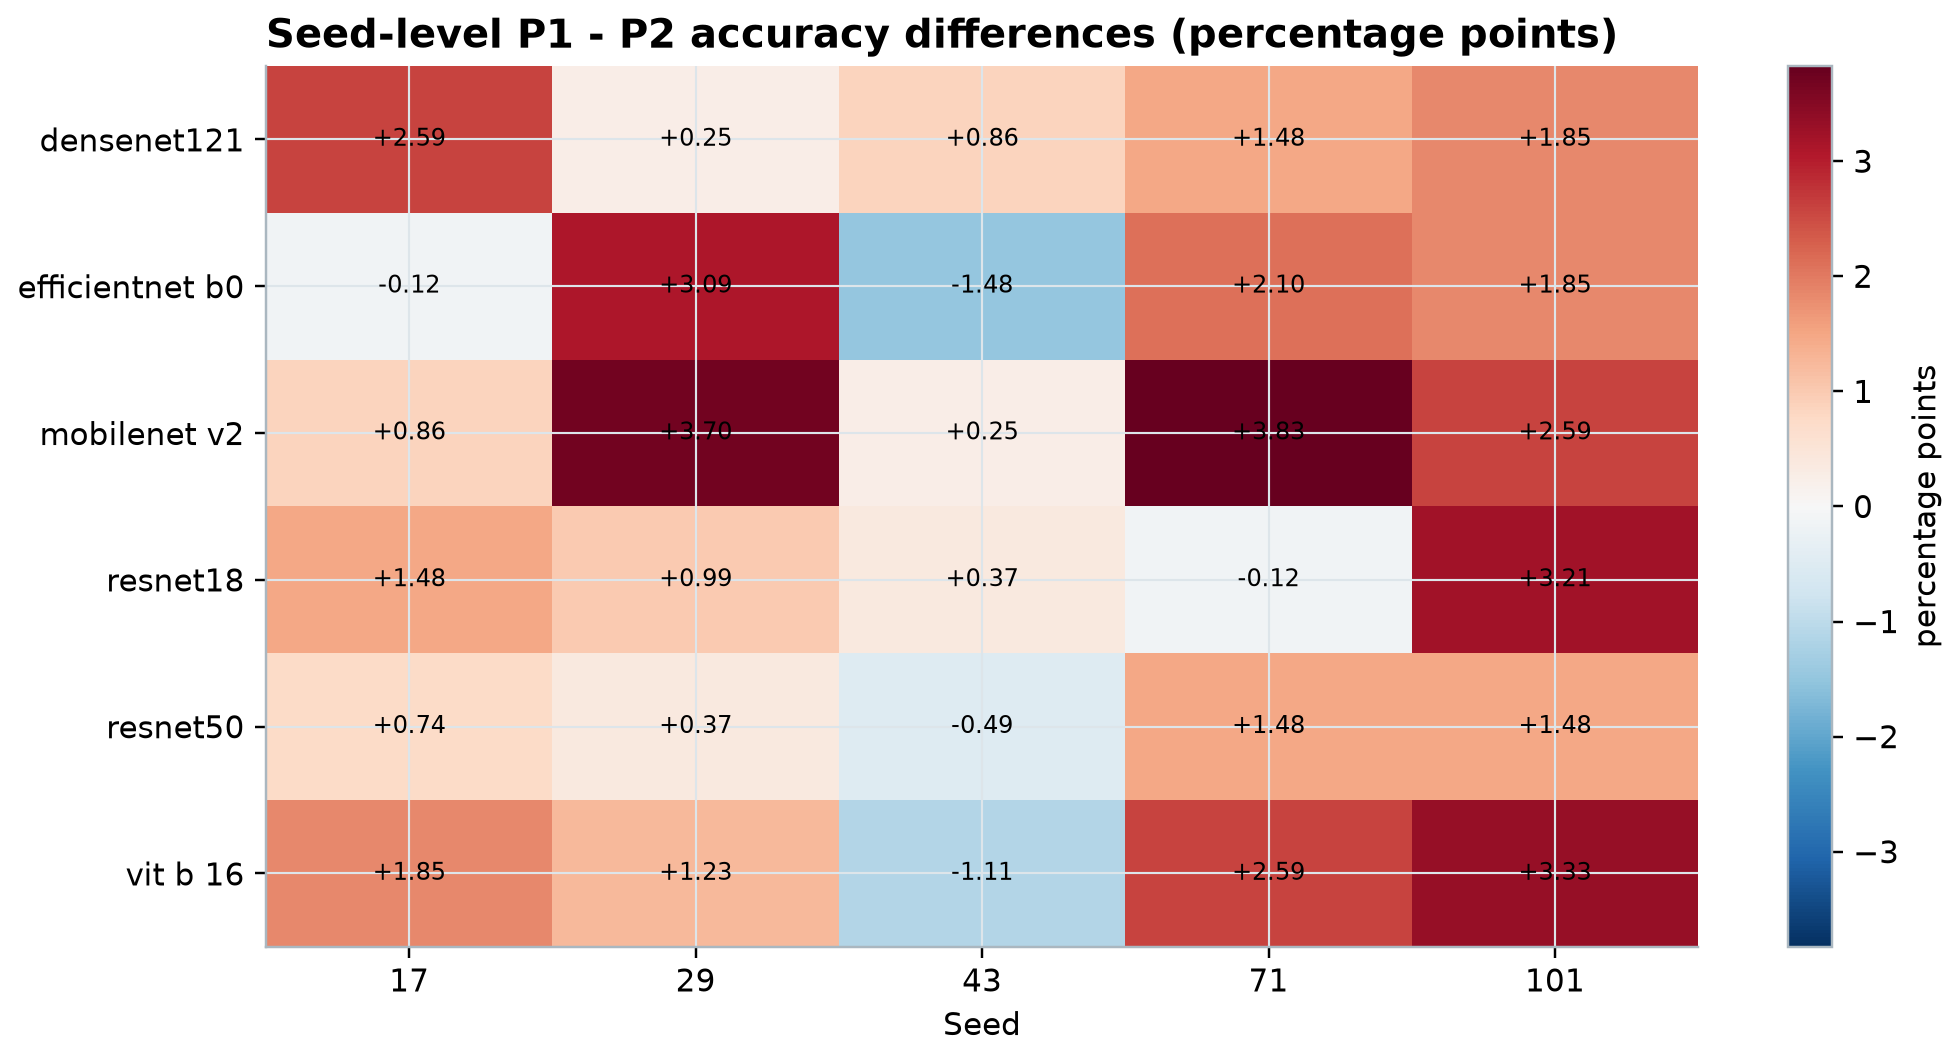
\includegraphics[width=\textwidth]{classification_seed_deltas.png}
\caption{Seed-level paired differences. This figure exposes the small effective sample size and the architecture-specific variability that an aggregate table can hide.}
\label{fig:classification-seeds}
\end{figure}

The registered monotonicity expectation was \protocol{P3}$\leq$\protocol{P2}$\leq$\protocol{P1}. Only ResNet-50 and ViT-B/16 satisfy it. The other four improve from \protocol{P2} to \protocol{P3} by 0.35--1.04 points. Those reversals are not deleted or relabeled: the corresponding \protocol{P2}$-$\protocol{P3} differences are $-0.67$, $-0.72$, $-1.04$, $-0.35$, $+0.52$, and $+0.02$ points in table order, and none has an adjusted confirmatory claim.

\begin{figure}[H]
\centering
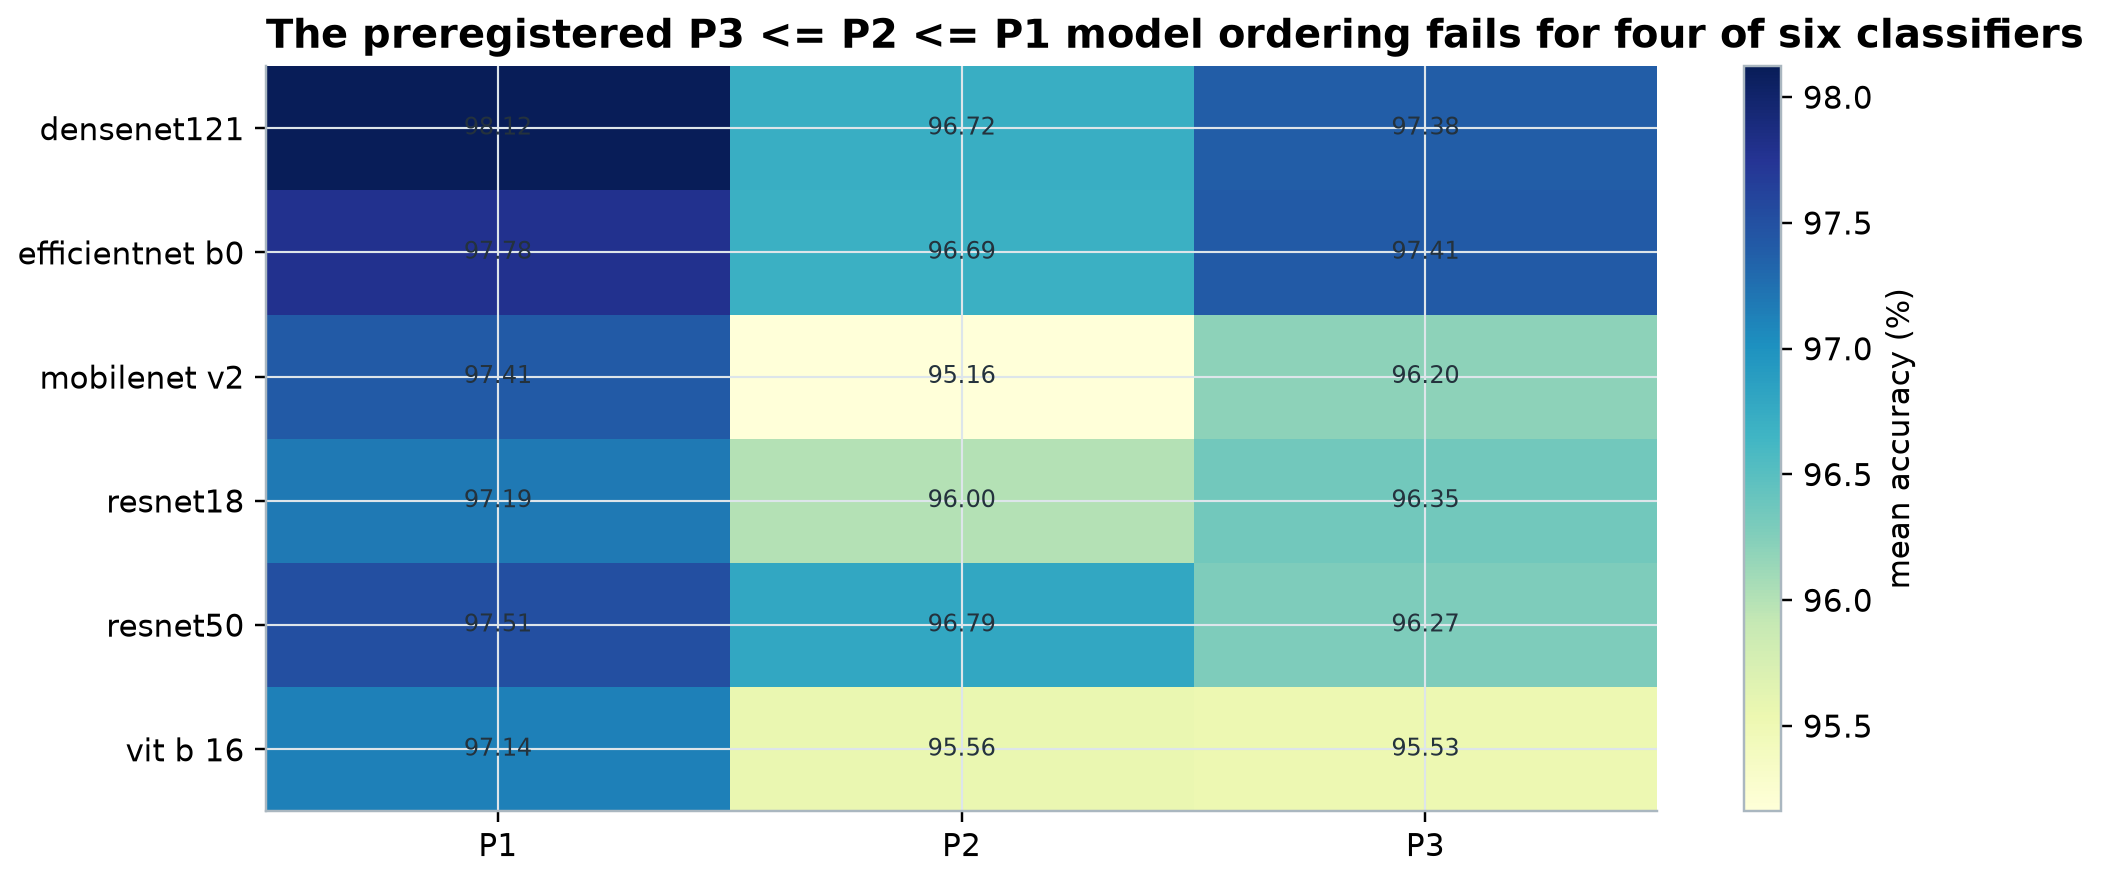
\includegraphics[width=\textwidth]{classification_ordering.png}
\caption{The registered ordering check. Cell values are the protocol means; the title records the gate outcome. Four of six architectures fail \protocol{P3}$\leq$\protocol{P2}$\leq$\protocol{P1}, so the acceptance contract correctly records one failed gate.}
\label{fig:classification-ordering}
\end{figure}

Architecture ranks are also unstable across \protocol{P1} and \protocol{P2}: Kendall's $\tau=0.467$ with bootstrap interval [0.071, 0.733] and $p=0.2722$; four of the 15 architecture pairs reverse. This is a descriptive warning that a benchmark split can alter conclusions about model selection even when absolute score differences look modest.

\section{What the classification rescore does and does not show}

The same-sign result across six architectures is scientifically suggestive and consistent with the structural mechanism. The five-seed paired variability is nevertheless too large for any architecture to pass the six-test BH family. The correct report is therefore: \emph{crop-disjoint scores were higher on average for every tested classifier, by 0.72--2.25 percentage points, but the preregistered architecture-wise confirmatory family did not establish individual effects after multiplicity correction.}

No classifier confusion matrix appears because the frozen result schema retains aggregate test metrics and epoch histories, but not per-sample predictions or model checkpoints. Generating such a matrix now would require a new experiment after the declared research stop. Omitting it is more faithful than reconstructing or simulating unobserved cells.

\section{Training behavior and compute}

\begin{figure}[H]
\centering
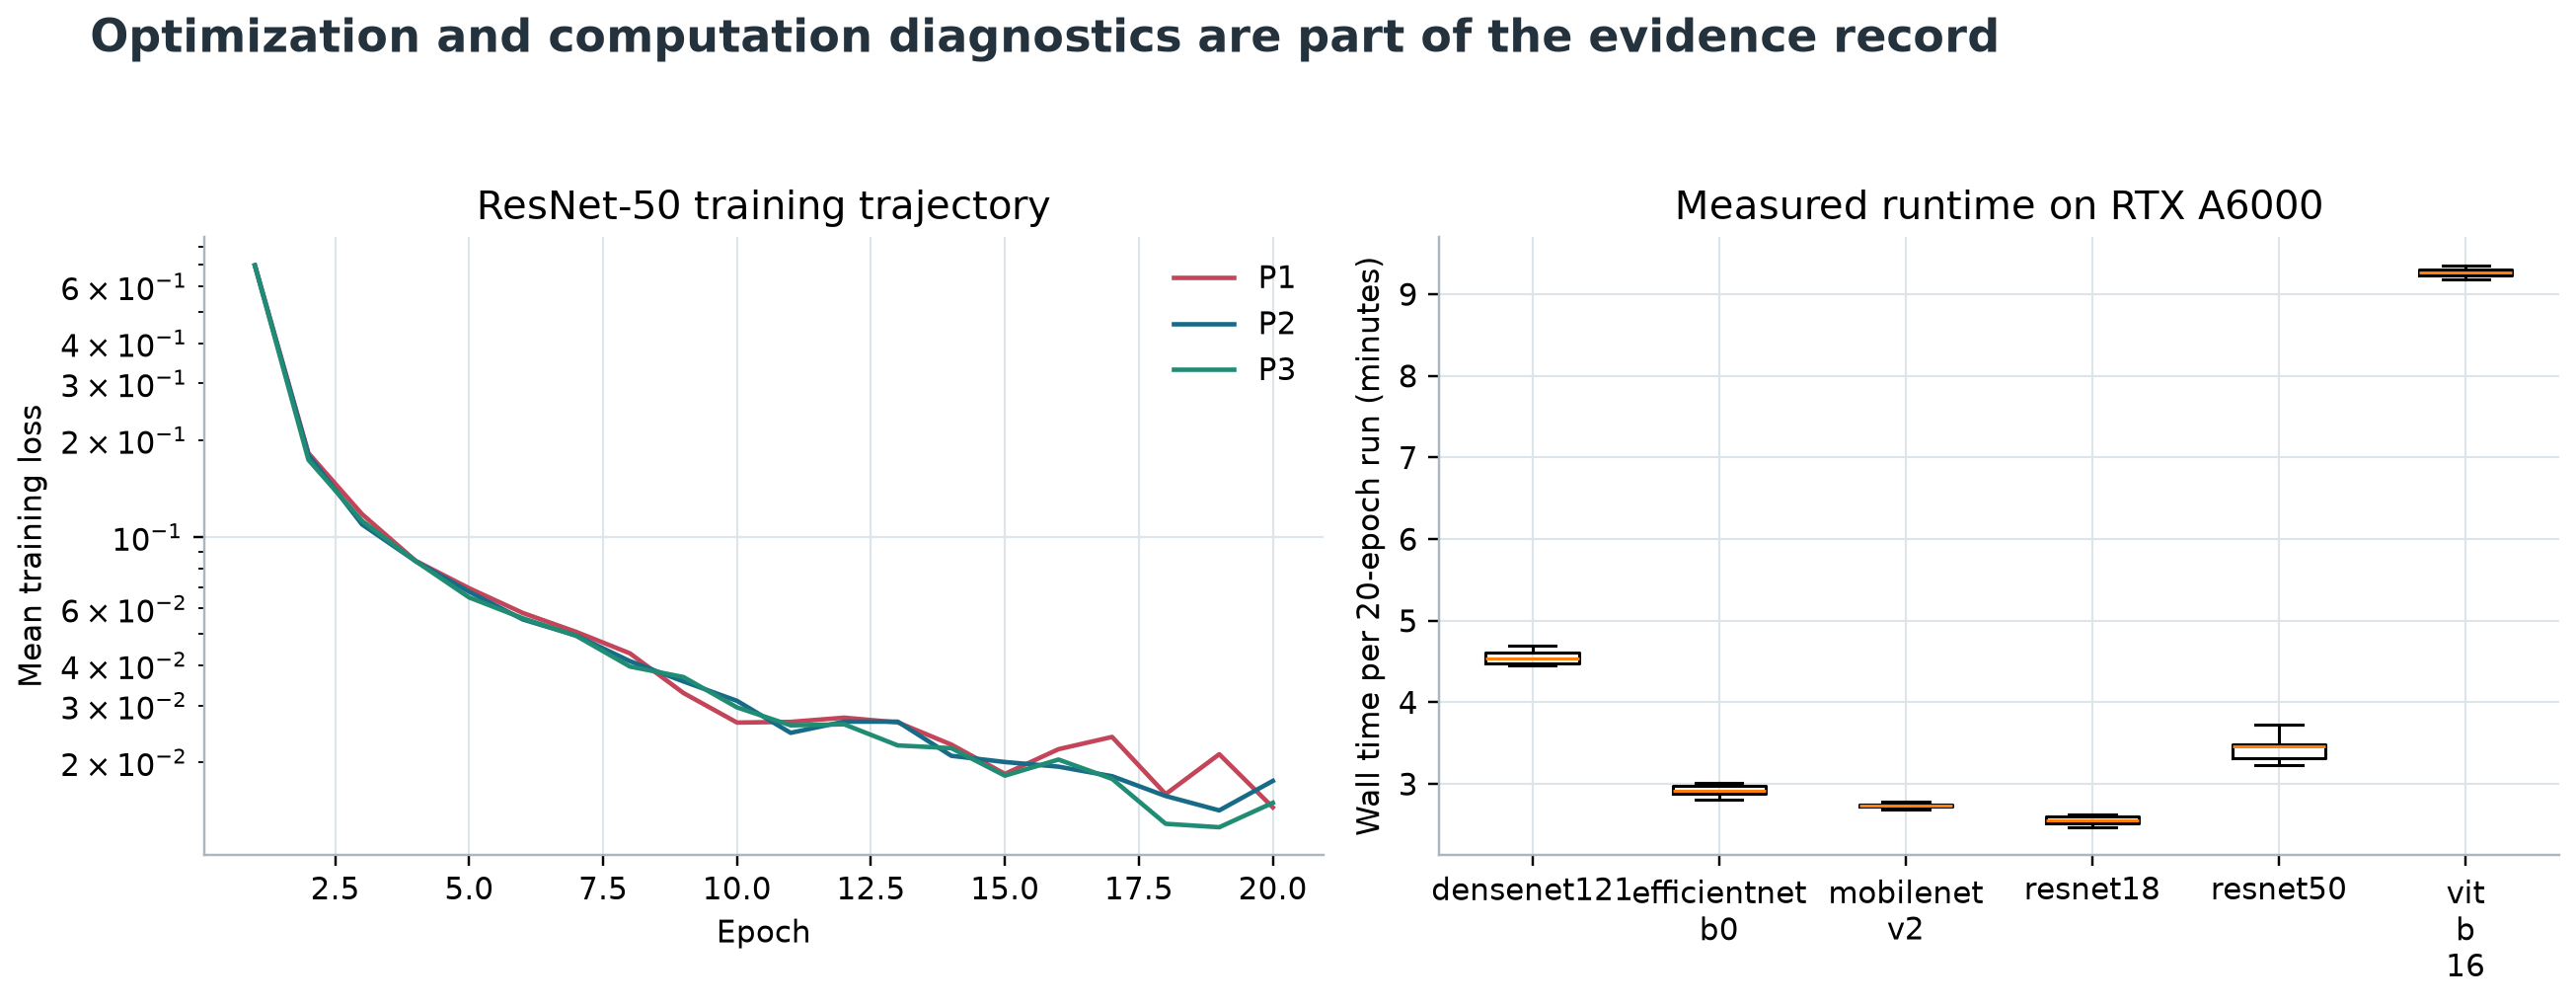
\includegraphics[width=\textwidth]{classification_training_runtime.png}
\caption{Classifier wall-clock summaries from the retained run JSON files. These are same-system measurements and should not be compared to timings reported on unrelated hardware.}
\label{fig:classification-runtime}
\end{figure}

The 120 retained classification runs consumed 8.48 summed run-hours. Because up to three jobs ran concurrently, this is computational work, not elapsed calendar duration. Shorter wall time does not imply a more accurate or better-calibrated model; it is included so the execution cost is auditable.

\chapter{Cx22 segmentation rescore}

\section{Why add a second task and dataset?}

Classification alone could leave two alternative explanations: perhaps the phenomenon is specific to SIPaKMeD, or perhaps it is specific to assigning a single label to a crop. Cx22 offers a different hierarchy and two pixel-level tasks. It therefore tests whether the split logic transfers to semantic and instance segmentation without pretending that its official split is the same estimand as the pooled stress test.

The pooled analysis treats all 1,320 released generated regions as the observation pool and the 514 CCEDD sources as parents. The protocol{OFFICIAL} arm uses only Cx22-Multi-Train (400 observations) and Cx22-Multi-Test (100 observations). These official train and test source-parent sets are disjoint. Pair is not added to the official test comparison: 55 of its source parents overlap Multi-Test and 233 overlap Multi-Train, with Jaccard similarities 0.126 and 0.475 respectively. Pooling and re-splitting is thus a downstream-reuse stress test, not an accusation that the authors' official Multi split is flawed.

\section{Targets and models}

The semantic target has two independent binary channels: cytoplasm and nucleus. Five encoder--decoder families are re-run: U-Net~\cite{ronneberger2015unet}, U-Net++~\cite{zhou2020unetplusplus}, DeepLabV3+~\cite{chen2018deeplabv3plus}, FPN~\cite{lin2017fpn}, and MAnet~\cite{fan2020manet}. ResNet-34 is the encoder except for DeepLabV3+, which uses ResNet-50. All encoders start from ImageNet weights. The output activation is not embedded in the network; logits are passed through sigmoid in the loss and evaluation code.

For image $i$, channel $c$, prediction probability $p_{icu}$, and binary target $y_{icu}$ at pixel $u$, the training objective is
\begin{align}
\mathcal L_{\mathrm{semantic}}
&=\mathcal L_{\mathrm{BCE}}+\mathcal L_{\mathrm{softDice}},\\
\mathcal L_{\mathrm{softDice}}
&=1-\frac{1}{2N}\sum_{i,c}
\frac{2\sum_u p_{icu}y_{icu}+1}
{\sum_u p_{icu}+\sum_u y_{icu}+1}.
\end{align}

The instance task uses Mask R-CNN with a ResNet-50 FPN backbone and its torchvision V2 implementation~\cite{he2017maskrcnn}. The classification and mask heads are replaced for one foreground category plus background. Ground-truth cytoplasm instances are reconstructed from the released MATLAB label structure before resizing. Empty instances after resizing are rejected rather than silently retained.

\section{Deterministic input construction}

All images and masks are resized to $256\times256$; RGB images use antialiased interpolation, while masks use nearest-neighbor interpolation. Training augmentation is determined by a SHA-256 digest of seed, epoch, and crop ID. Digest bits choose horizontal flip, vertical flip, and one of four right-angle rotations. This produces per-epoch augmentation without relying on worker scheduling order. Images are ImageNet-normalized; masks remain binary.

The original JPEGs and generated masks were packed into memory-mappable arrays, each named in a provenance manifest with SHA-256 hashes and a cache version. This was not a scientific transformation. It removed repeated JPEG/MATLAB/NFS decoding from the inner loop while making the exact input bytes auditable.

\begin{table}[H]
\centering
\caption{Cx22 segmentation execution settings.}
\label{tab:cx22-hparams}
\begin{tabular}{lll}
\toprule
Item & Semantic & Instance \\
\midrule
Image size & $256\times256$ & $256\times256$ \\
Epochs & 30 & 30 \\
Batch size & 16 & 2 (test batch 1) \\
Optimizer & AdamW & AdamW \\
Learning rate & $10^{-4}$ fixed & $10^{-4}$ fixed \\
Weight decay & $10^{-4}$ & $10^{-4}$ \\
Precision & FP16 except MAnet FP32 & FP16 \\
Endpoint schedule & every epoch; final retained & final epoch only \\
Checkpointing & every epoch & every 5 epochs \\
Seeds & 17, 29, 43, 71, 101 & 17, 29, 43, 71, 101 \\
Hardware & \multicolumn{2}{l}{NVIDIA RTX A6000; at most three concurrent GPU jobs} \\
\bottomrule
\end{tabular}
\end{table}

\section{Semantic metrics}

Probabilities are thresholded at 0.5. For predicted set $A$ and target set $B$,
\begin{equation}
\operatorname{Dice}(A,B)=\frac{2|A\cap B|}{|A|+|B|},\qquad
\operatorname{IoU}(A,B)=\frac{|A\cap B|}{|A\cup B|}.
\end{equation}
The primary semantic value first averages cytoplasm and nucleus Dice within each image, then averages over test images. This prevents a large cytoplasm region from numerically drowning the smaller nucleus. Channel-specific Dice and IoU are retained as diagnostic endpoints.

\section{Instance matching metric}

Predictions with object score below 0.5 are discarded. Let $D_{jk}$ be Dice between predicted instance $j$ and ground-truth instance $k$. The Hungarian assignment~\cite{kuhn1955hungarian} maximizes
\begin{equation}
\max_{\pi}\sum_{(j,k)\in\pi}D_{jk}
\end{equation}
subject to one-to-one matching. Every unmatched ground-truth instance receives Dice and IoU zero. The primary image value is the mean over that image's ground-truth instances; images are then averaged. Recall@0.70 is the fraction of ground-truth instances whose matched Dice is at least 0.70. This endpoint penalizes missed cells and does not allow an image with many easy instances to dominate the result.

\begin{lstlisting}[style=cyto,caption={Exact logic of the matched-instance endpoint.},label={lst:instance-metric}]
keep predictions with confidence >= 0.50
threshold predicted and target masks at 0.50
compute all predicted-by-target Dice values on the GPU
solve maximum-weight one-to-one assignment
write matched Dice into a zero vector of length n_targets
average the vector within the image
average image means over the test set
\end{lstlisting}

\section{Semantic results}

\begin{table}[H]
\centering
\caption{Cx22 semantic macro-Dice (\%), mean $\pm$ sample SD over five seeds. The official column uses a different 400/100 sample and is descriptive, not a paired protocol contrast.}
\label{tab:cx22-semantic}
\small
\begin{tabular}{lrrrrr}
\toprule
Model & \protocol{P1} & \protocol{P1$'$} & \protocol{P2} & \protocol{P3} & \protocol{OFFICIAL} \\
\midrule
DeepLabV3+ & 88.90$\pm$0.45 & 88.84$\pm$0.45 & 88.64$\pm$0.34 & 88.10$\pm$0.38 & 82.96$\pm$1.54 \\
FPN & 88.90$\pm$0.43 & 88.97$\pm$0.55 & 88.89$\pm$0.48 & 88.33$\pm$0.30 & 84.43$\pm$0.33 \\
MAnet & 90.03$\pm$0.60 & 90.07$\pm$0.63 & 89.97$\pm$0.45 & 89.63$\pm$0.21 & 85.50$\pm$1.41 \\
U-Net & 90.29$\pm$0.48 & 90.32$\pm$0.52 & 89.99$\pm$0.52 & 89.77$\pm$0.16 & 85.64$\pm$0.58 \\
U-Net++ & 90.56$\pm$0.51 & 90.58$\pm$0.54 & 90.38$\pm$0.35 & 90.05$\pm$0.21 & 87.30$\pm$1.13 \\
\bottomrule
\end{tabular}
\end{table}

\begin{figure}[H]
\centering
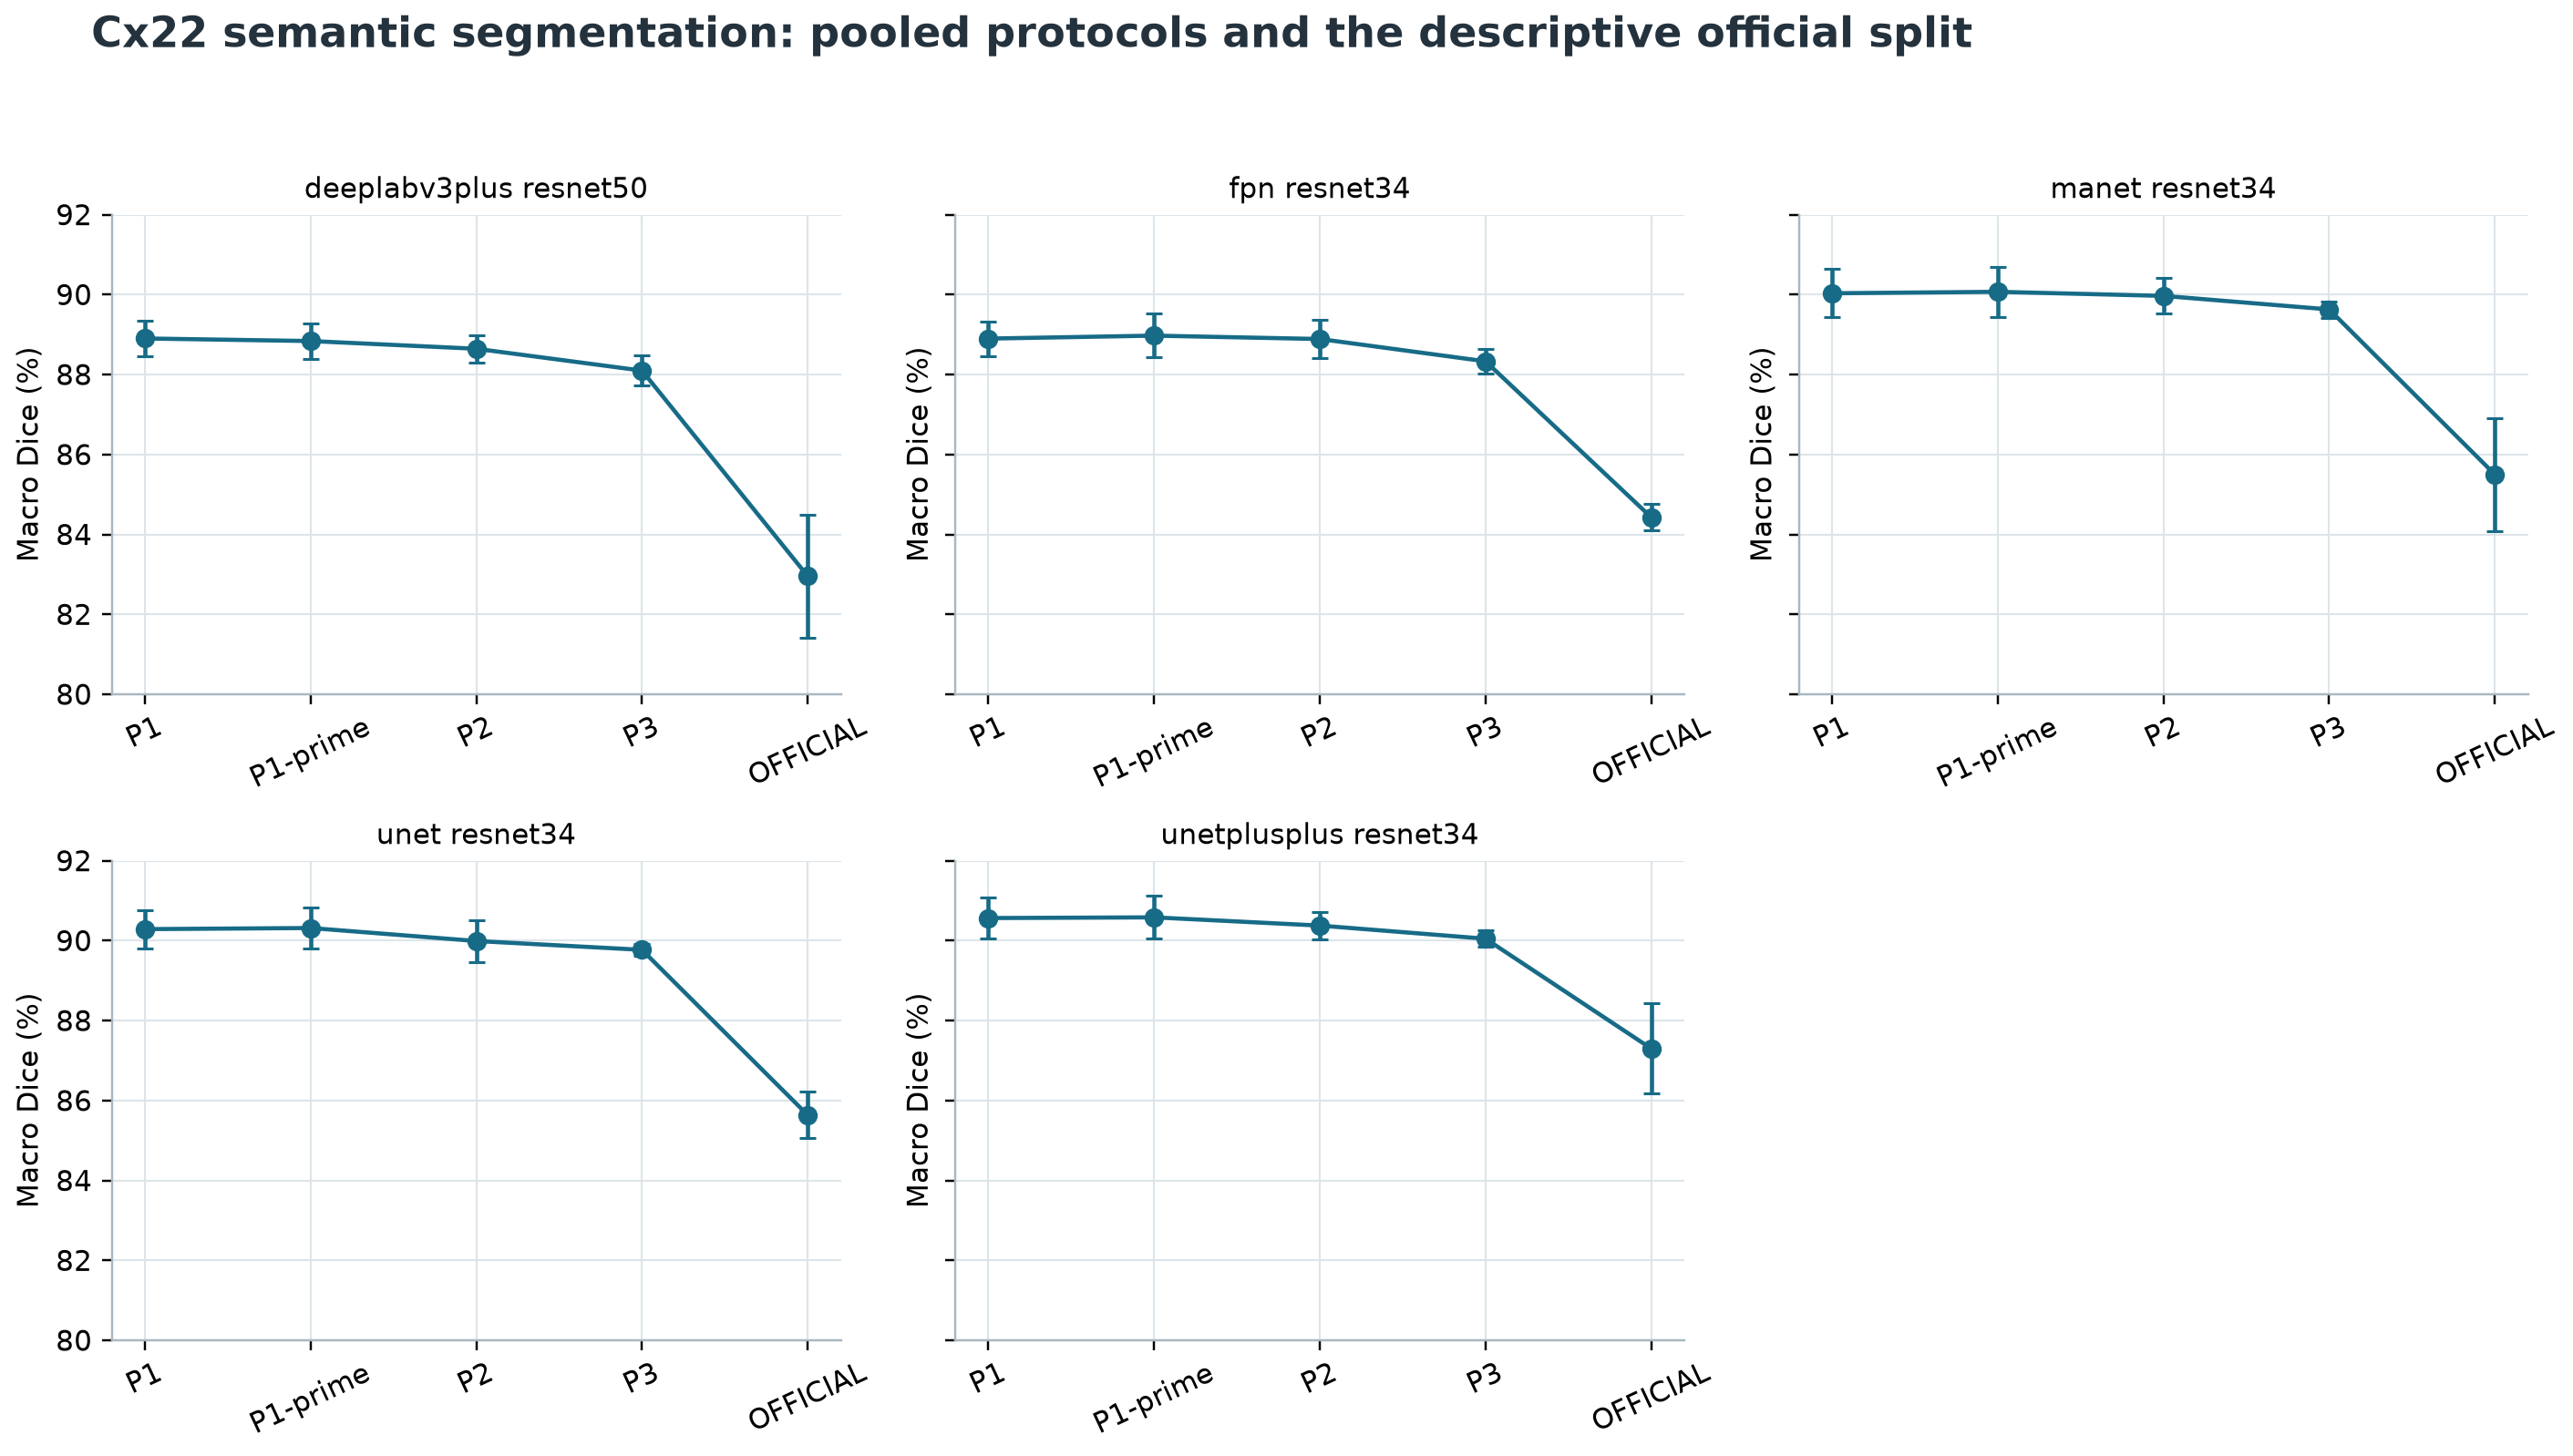
\includegraphics[width=\textwidth]{cx22_semantic_scores.png}
\caption{Cx22 semantic macro-Dice by architecture and protocol. The official arm is visually separated because it is not a same-observation contrast.}
\label{fig:cx22-semantic}
\end{figure}

\begin{figure}[H]
\centering
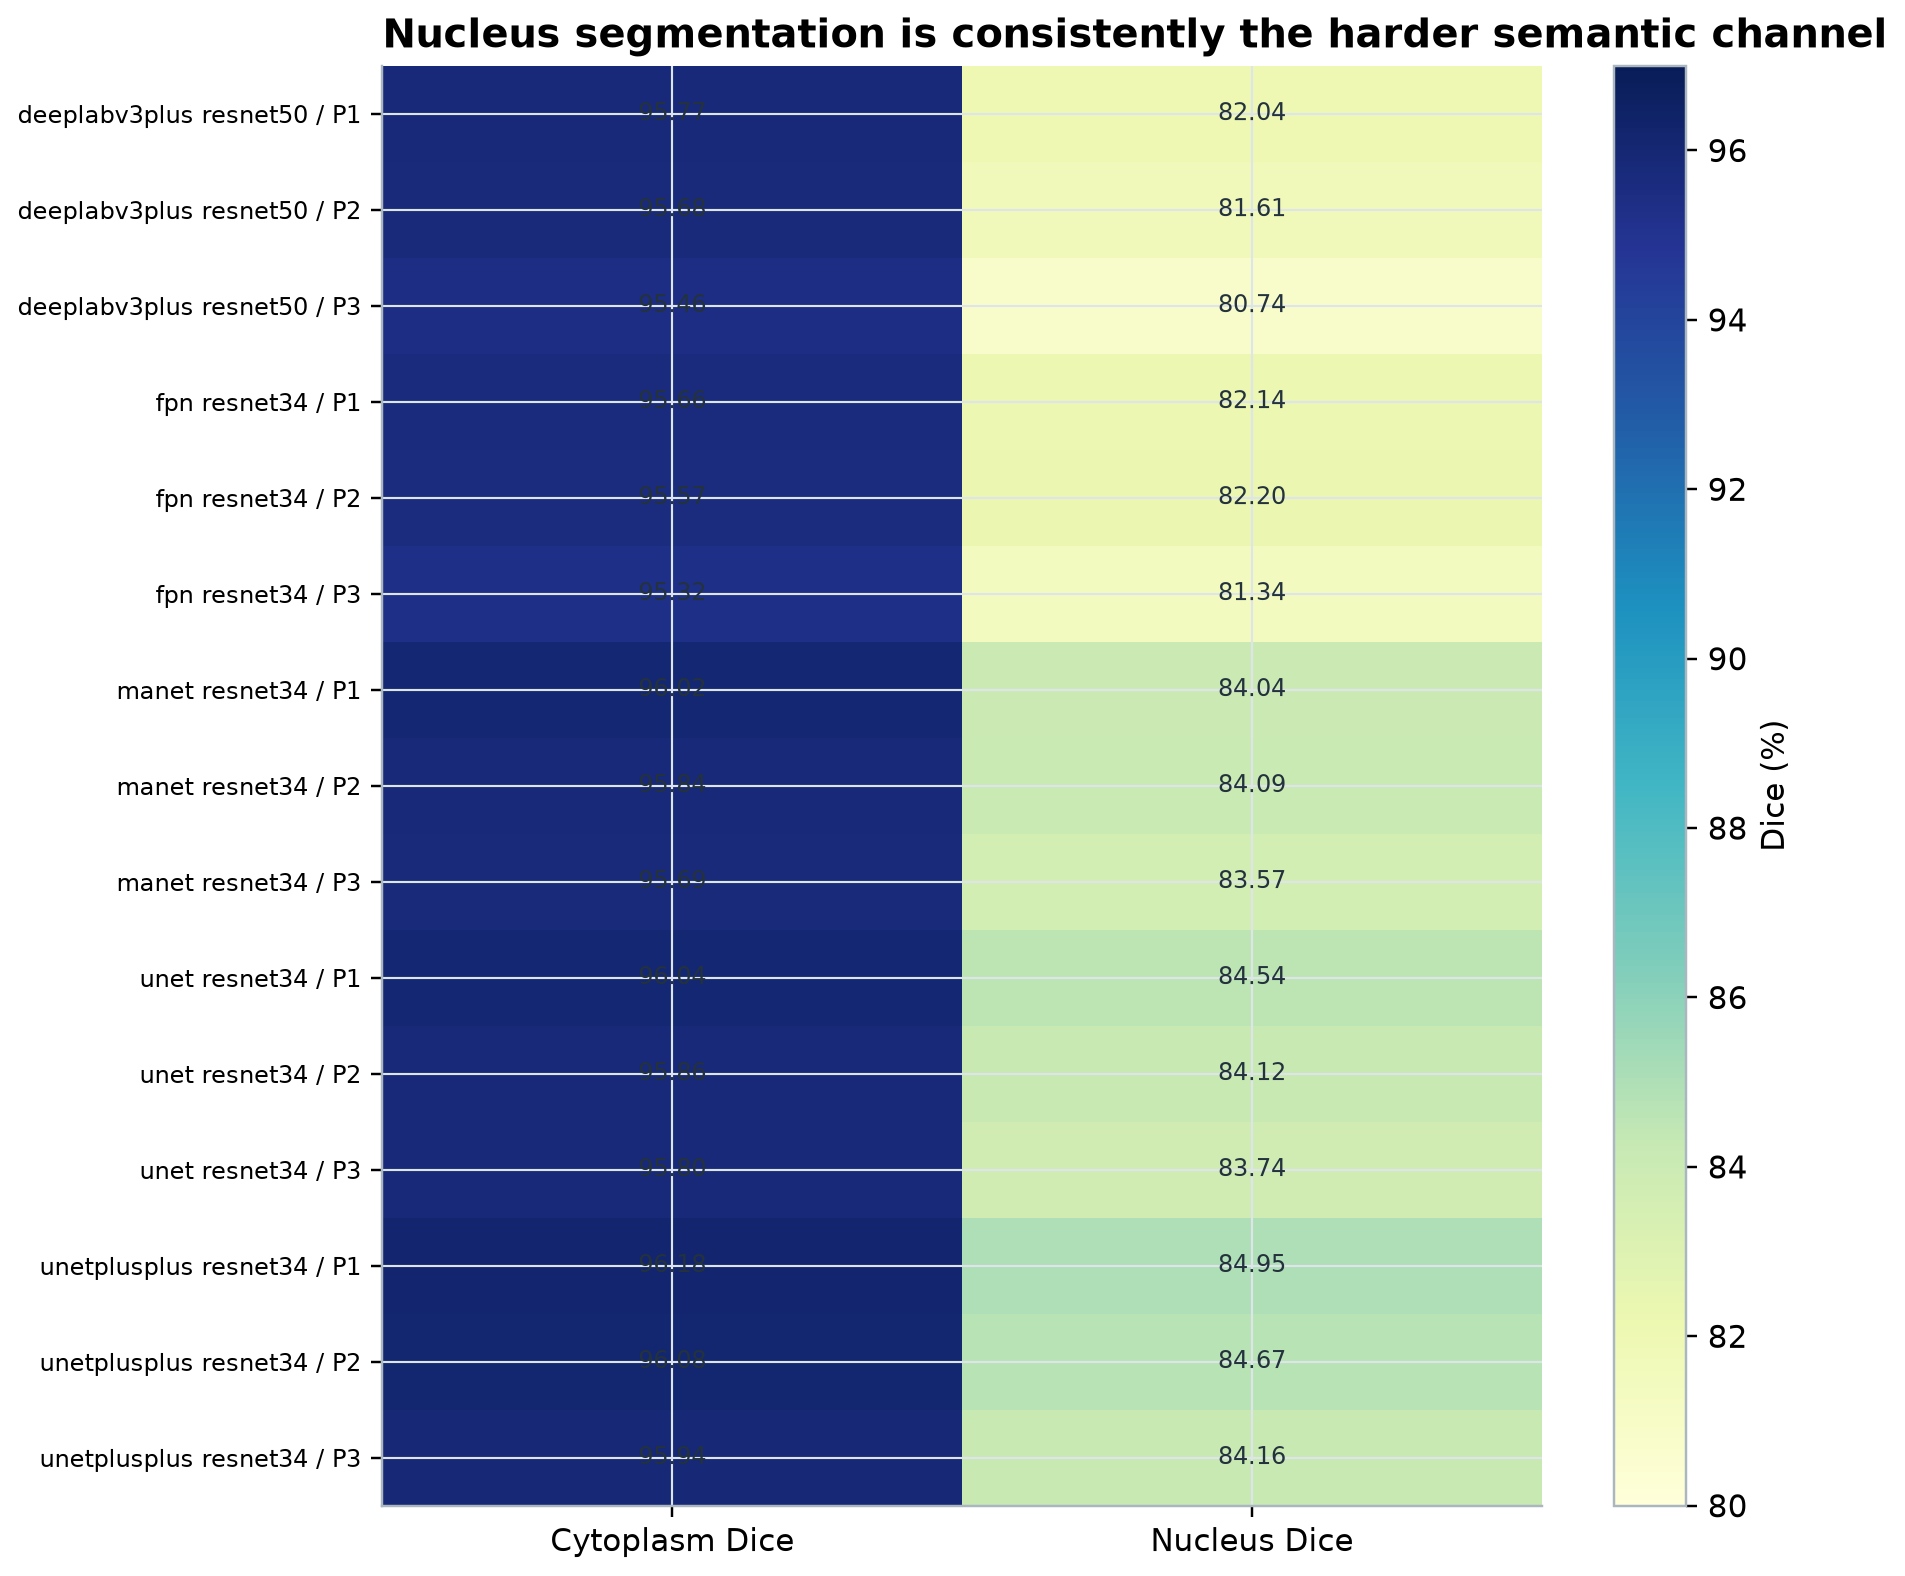
\includegraphics[width=\textwidth]{cx22_channel_heatmap.png}
\caption{Channel-level Dice makes the central difficulty visible: nuclei are consistently harder than cytoplasm. This is the segmentation analogue of a confusion-matrix diagnostic and uses retained aggregate channel measurements, not invented pixel predictions.}
\label{fig:cx22-channels}
\end{figure}

U-Net++ is best in every pooled protocol and on the official Multi arm. The channel breakdown explains the lower official macro score: across models, cytoplasm Dice is roughly 94--95\% while nucleus Dice is roughly 72--79\%. Nuclei are smaller, so a fixed boundary displacement consumes a larger fraction of their area; faint staining and overlap also make the boundary less stable. This is a checkable data property visible in the released masks rather than a generic explanation added after the fact.

\section{Instance results}

\begin{table}[H]
\centering
\caption{Cx22 matched-instance Dice (\%), mean $\pm$ sample SD over five seeds.}
\label{tab:cx22-instance}
\small
\begin{tabular}{lrrrrr}
\toprule
Model & \protocol{P1} & \protocol{P1$'$} & \protocol{P2} & \protocol{P3} & \protocol{OFFICIAL} \\
\midrule
Mask R-CNN & 92.10$\pm$0.52 & 92.05$\pm$0.52 & 91.59$\pm$0.42 & 91.11$\pm$1.09 & 92.29$\pm$0.32 \\
Mask R-CNN V2 & 91.99$\pm$0.57 & 91.95$\pm$0.58 & 91.36$\pm$0.82 & 90.60$\pm$0.52 & 92.18$\pm$0.71 \\
\bottomrule
\end{tabular}
\end{table}

\begin{figure}[H]
\centering
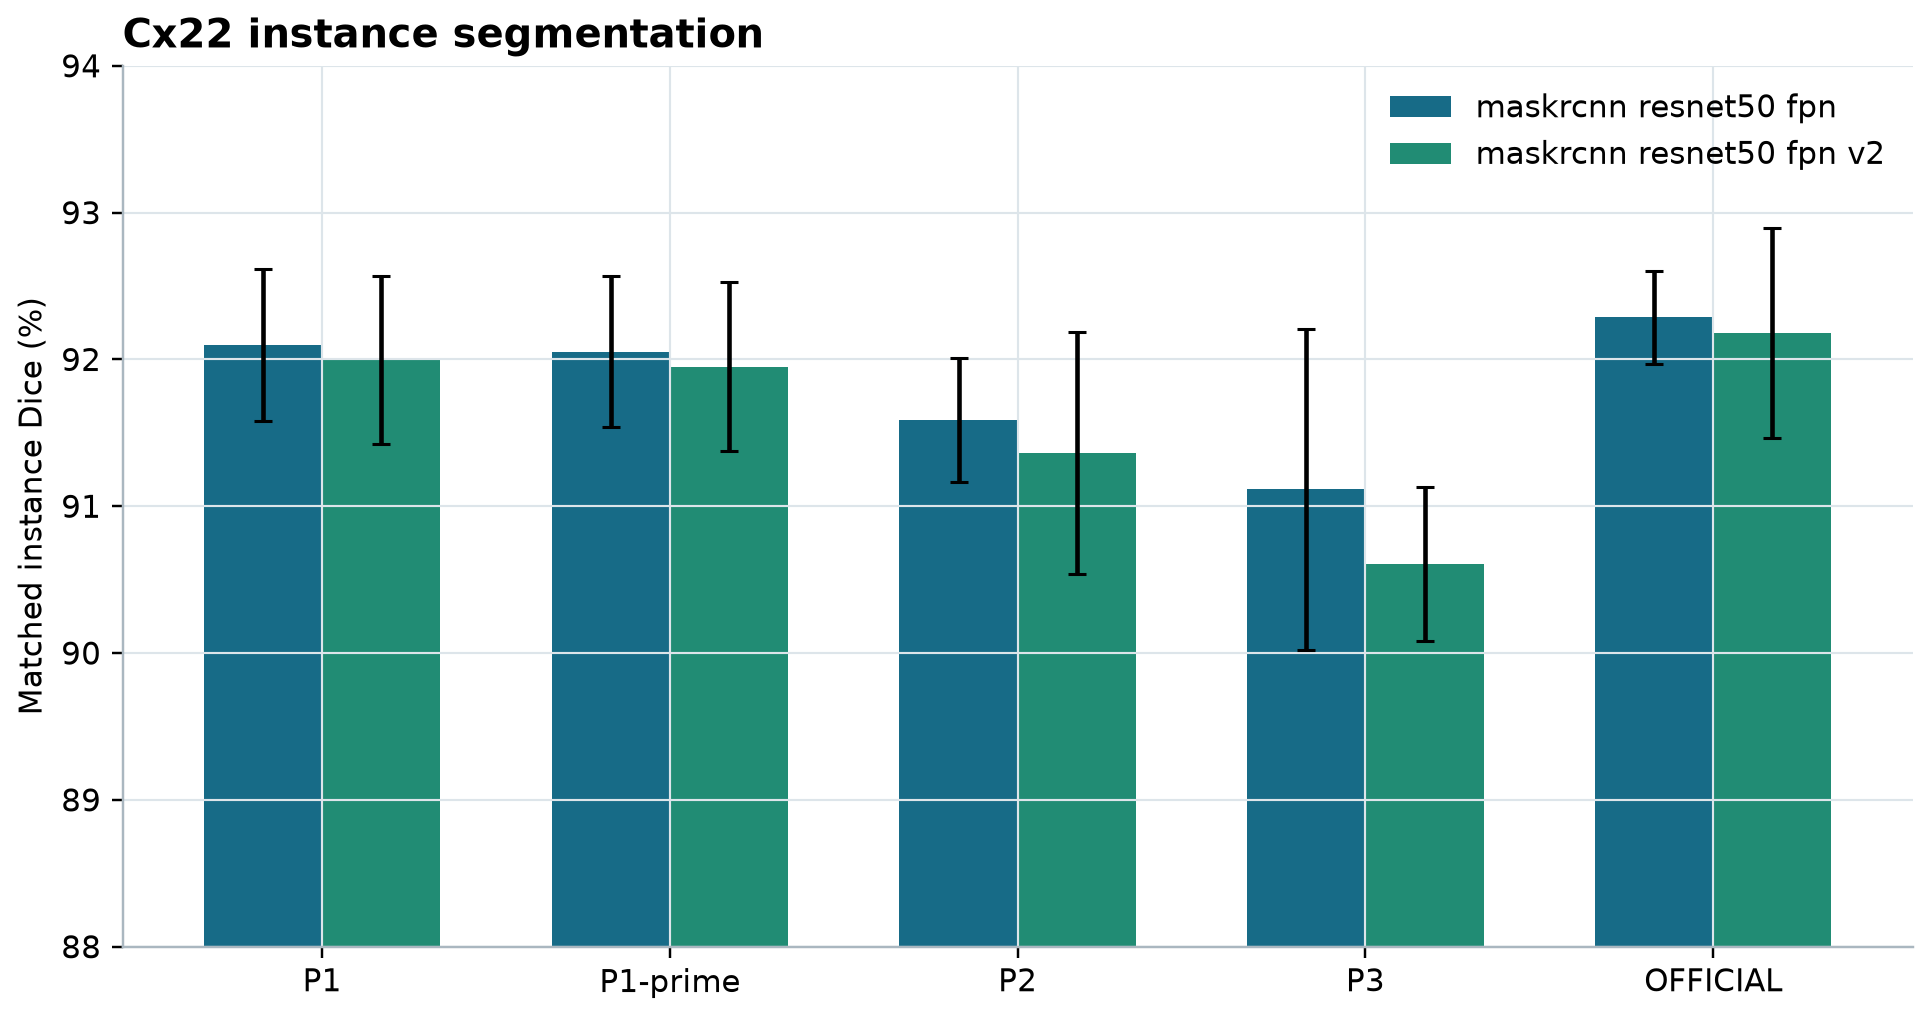
\includegraphics[width=\textwidth]{cx22_instance_scores.png}
\caption{Cx22 matched-instance Dice. Both Mask R-CNN variants follow the complete registered \protocol{P3}$\leq$\protocol{P2}$\leq$\protocol{P1} ordering.}
\label{fig:cx22-instance}
\end{figure}

Unlike SIPaKMeD classification, all seven Cx22 architecture/task rows satisfy the registered ordering. The differences are still small: \protocol{P1}$-$\protocol{P2} is 0.01--0.30 percentage points for semantic models and 0.51--0.63 points for instance models.

\section{Inference and rank stability}

\begin{table}[H]
\centering
\caption{Primary Cx22 \protocol{P1}$-$\protocol{P2} contrasts. Values are mean $\pm$ SD percentage points; $q$ is within the task-specific preregistered family. Effect is Cohen's $d_z$ except DeepLabV3+, whose non-normal seed differences trigger rank-biserial effect size.}
\label{tab:cx22-primary}
\small
\begin{tabular}{llrrrr}
\toprule
Task & Model & Mean$\pm$SD & Raw $p$ & BH $q$ & Effect \\
\midrule
Semantic & DeepLabV3+ & 0.258$\pm$0.418 & 0.3125 & 0.8458 & 0.600$^{\dagger}$ \\
Semantic & FPN & 0.010$\pm$0.468 & 0.9625 & 0.9625 & 0.022 \\
Semantic & MAnet & 0.065$\pm$0.450 & 0.7612 & 0.8458 & 0.146 \\
Semantic & U-Net & 0.297$\pm$0.767 & 0.4353 & 0.8458 & 0.387 \\
Semantic & U-Net++ & 0.188$\pm$0.406 & 0.3582 & 0.8458 & 0.464 \\
Instance & Mask R-CNN & 0.509$\pm$0.581 & 0.1220 & 0.2440 & 0.875 \\
Instance & Mask R-CNN V2 & 0.630$\pm$1.204 & 0.3068 & 0.3116 & 0.523 \\
\bottomrule
\multicolumn{6}{l}{\footnotesize $^{\dagger}$rank-biserial correlation; all other effects are Cohen's $d_z$.}
\end{tabular}
\end{table}

\begin{figure}[H]
\centering
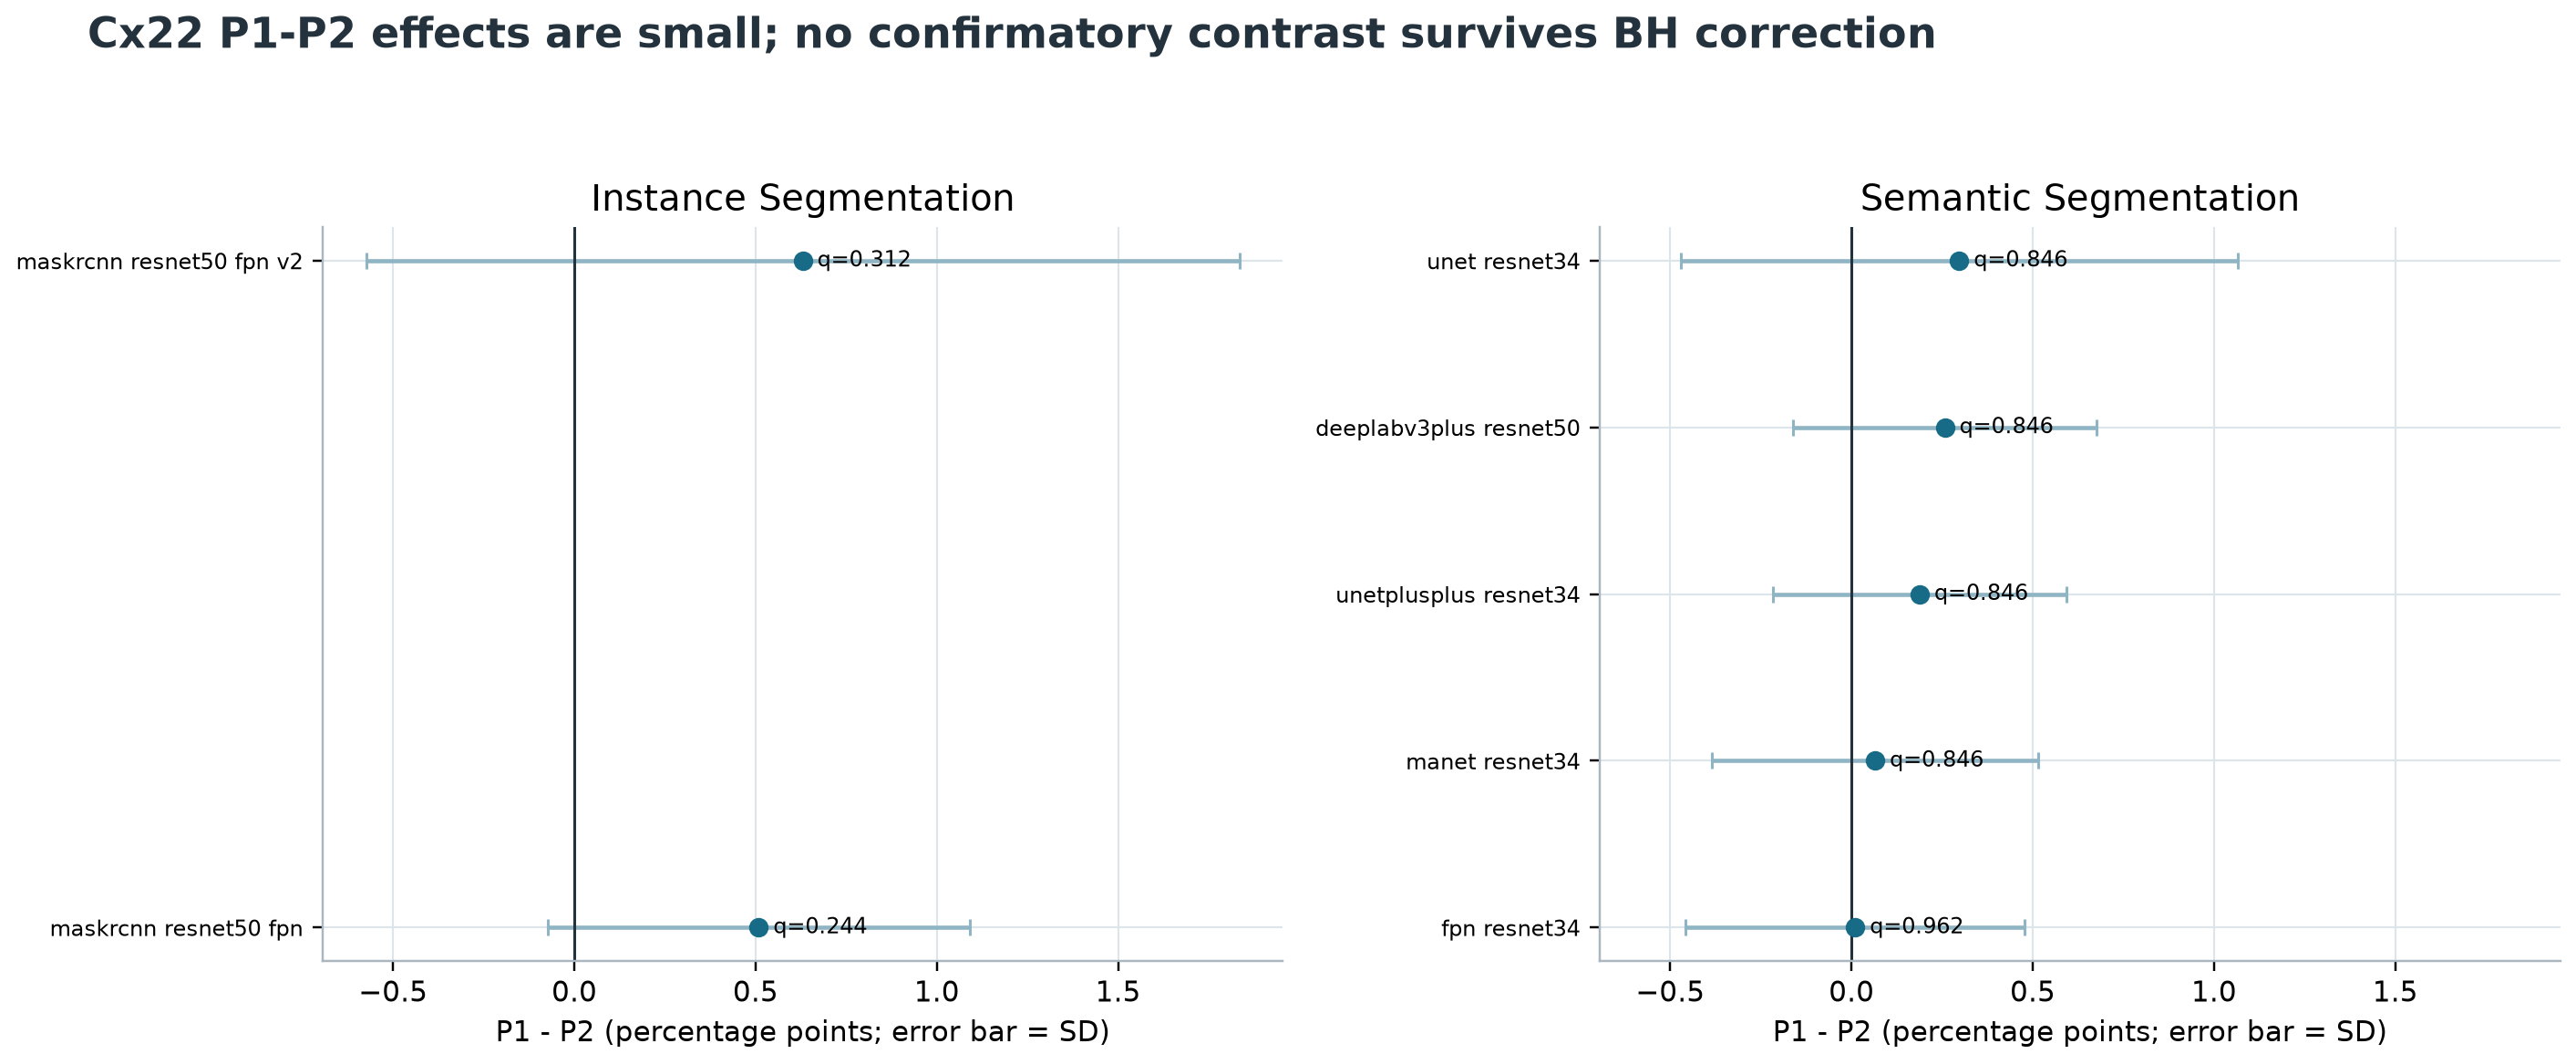
\includegraphics[width=\textwidth]{cx22_contrasts.png}
\caption{Cx22 paired contrast overview. Positive values favor the crop-level protocol. The plot separates point-estimate consistency from multiplicity-adjusted evidence.}
\label{fig:cx22-contrasts}
\end{figure}

No primary Cx22 test survives BH correction. The size-matched \protocol{P1$'$}$-$\protocol{P2} Mask R-CNN contrast has raw $p=0.0377$, $d_z=1.368$, and $q=0.1508$; it is not promoted to a significant claim. In the explicitly secondary \protocol{P2}$-$\protocol{P3} family, FPN has raw $p=0.0226$ and $d_z=1.613$; it remains secondary and is not used to rescue the main conclusion.

Semantic model ranking is comparatively stable: Kendall's $\tau=0.8$ with bootstrap interval [0.6, 1.0], $p=0.0833$, and one of ten model pairs reordered. With only two instance models, $\tau=1.0$ but its bootstrap interval spans [$-1$,1], which is appropriately uninformative.

\section{Training failures, recovery, and runtime}

The first MAnet \protocol{P1}, seed-17 attempts produced non-finite losses at epochs 23 and 24 under FP16, despite dynamic loss scaling. Retaining an epoch-22 model or changing only that seed would have biased the matrix. The matrix stopped at 100 of 175 cells, the failure was amended in writing, and every MAnet cell was restarted in FP32 from its fixed seed. The corrected runs also set \artifact{CUBLAS_WORKSPACE_CONFIG=:4096:8} before any corrected MAnet or instance result existed.

Instance segmentation exposed a different failure: not numerical instability, but pipeline starvation. Per-epoch test inference, CPU pairwise mask matching, and network-filesystem checkpoint writes made GPUs wait. The final endpoint was already preregistered, so evaluation was restricted to the final epoch, exact binary intersections moved to the GPU, checkpoints became five-epoch recovery files, and immutable arrays were staged locally. These changes preserved the endpoint and substantially improved utilization; they did not alter splits, seeds, models, thresholds, or the final metric.

\begin{figure}[H]
\centering
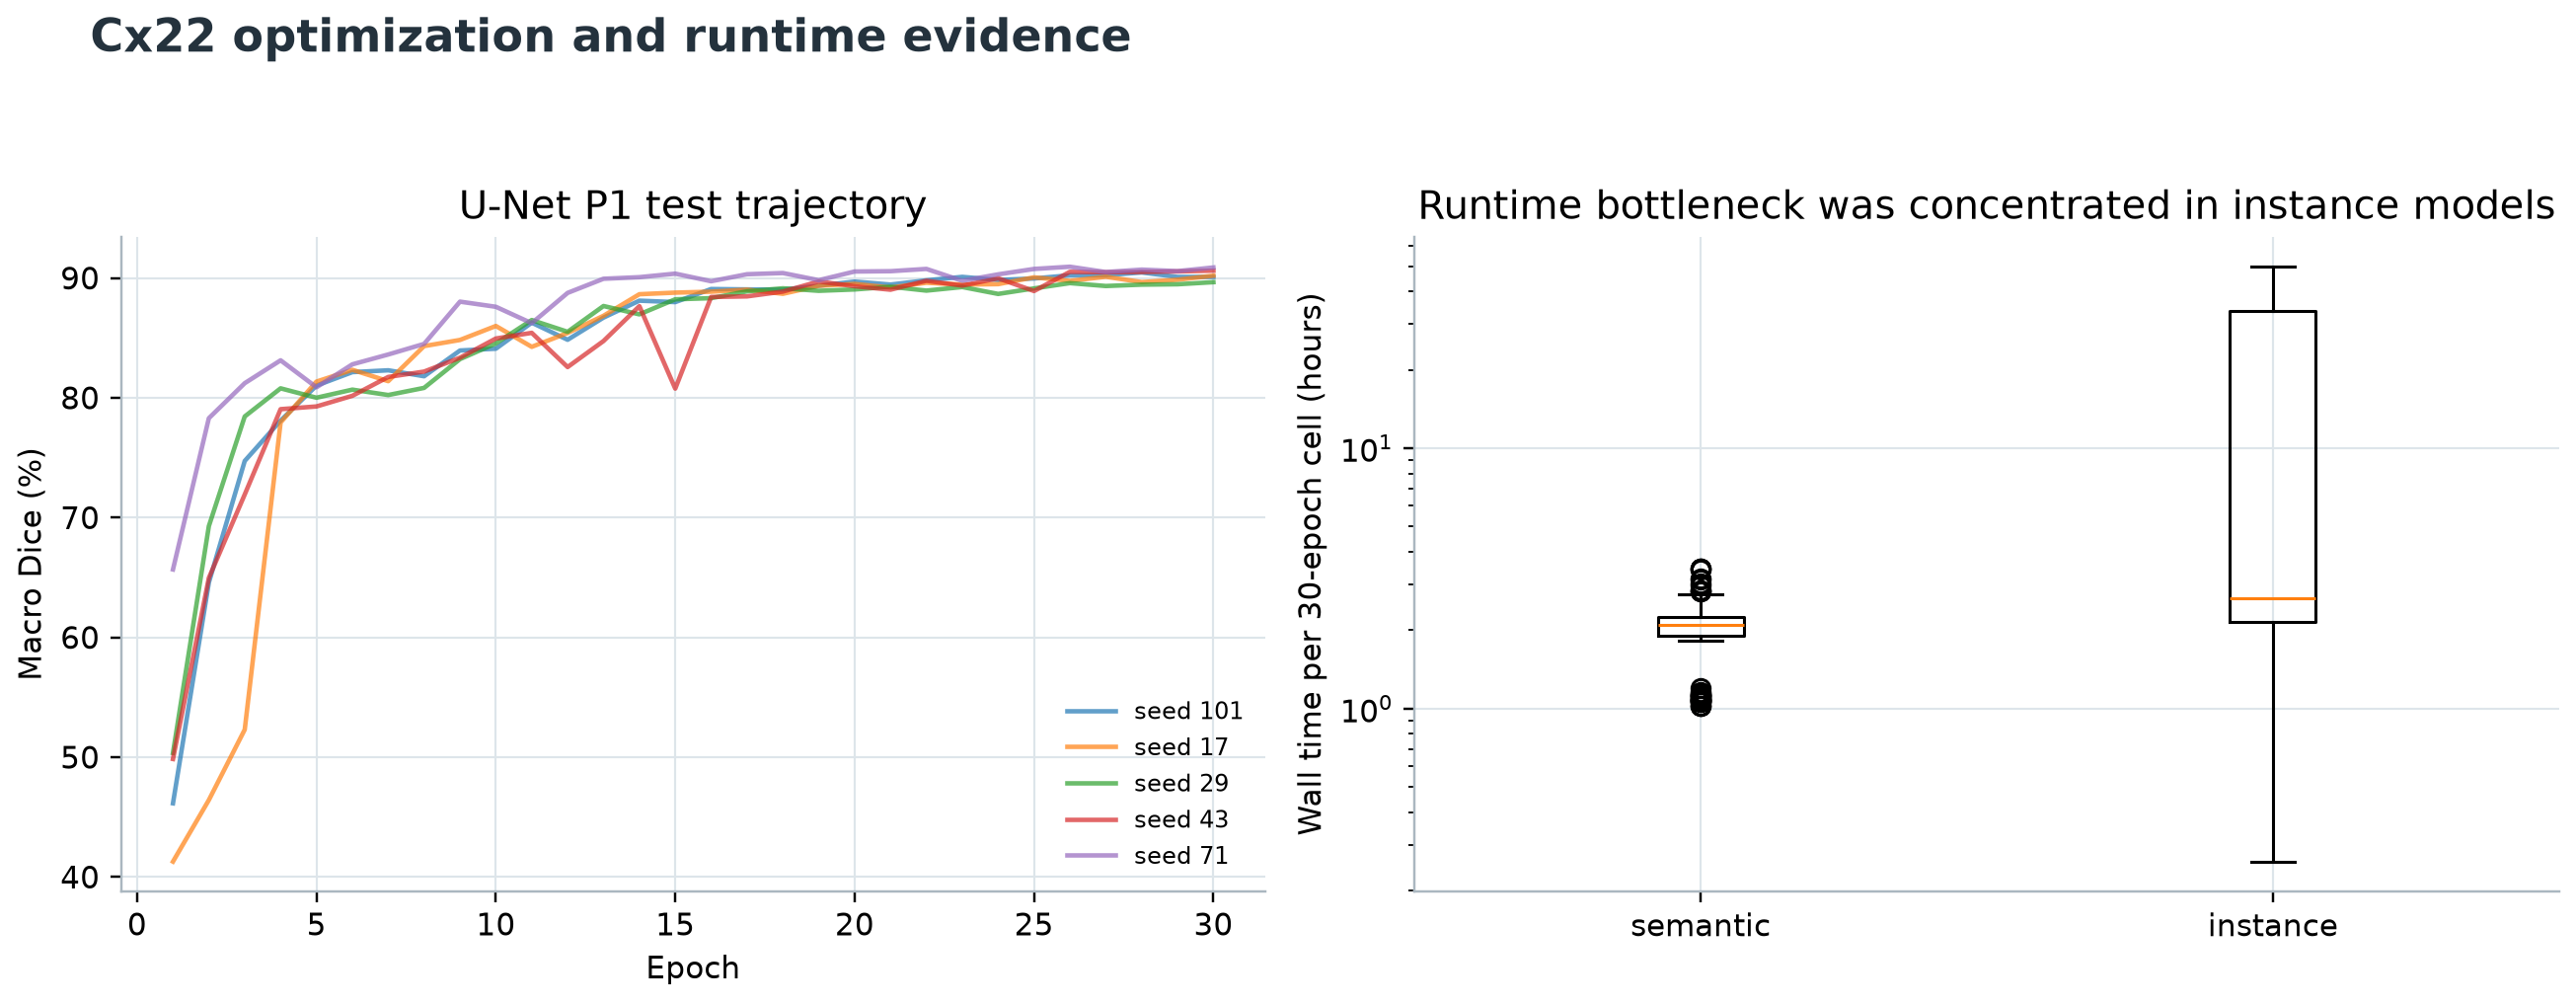
\includegraphics[width=\textwidth]{cx22_training_runtime.png}
\caption{Cx22 run-time distribution. Instance segmentation dominates the computational cost and has a long tail; the plot makes the operational bottleneck explicit.}
\label{fig:cx22-runtime}
\end{figure}

The 125 semantic cells consumed 253.33 summed run-hours, with median cell time 2.09 hours. The 50 instance cells consumed 646.76 summed run-hours, with median 2.64 hours and range 0.258--49.79 hours. The complete Cx22 matrix consumed 900.08 summed run-hours. Up to three jobs were concurrent, so the sum is not wall-clock project duration.

As in classification, final model weights and per-pixel predictions were not retained after the completed JSON was written. Figure~\ref{fig:cx22-labels} therefore visualizes real released ground truth, not a simulated qualitative prediction. A post-hoc prediction gallery would require fresh inference and is deliberately outside the frozen record.

\chapter{Statistical analysis in full}

\section{The experimental unit is the seed-paired run}

Every reported neural summary uses the five fixed seeds 17, 29, 43, 71, and 101 and gives the arithmetic mean with sample standard deviation ($n-1$ denominator). The protocol contrast is paired by seed. This pairing removes seed-to-seed variation that affects both arms and prohibits a favorable run in one protocol from being compared with an unrelated run in another.

For values $m_s$ over $S=5$ seeds,
\begin{equation}
\bar m=\frac{1}{S}\sum_{s=1}^{S}m_s,\qquad
s_m=\sqrt{\frac{1}{S-1}\sum_{s=1}^{S}(m_s-\bar m)^2}.
\end{equation}
A summary is suppressed if fewer than five seeds are present. This is enforced in code rather than remembered during table writing.

\section{Test-selection rule}

The preregistered rule first applies Shapiro--Wilk~\cite{shapiro1965normality} to the five paired differences. If $p\geq0.05$, a two-sided paired $t$-test is emitted; otherwise a two-sided Wilcoxon signed-rank test~\cite{wilcoxon1945rank} is emitted. The effect is Cohen's $d_z$ for a $t$-test and rank-biserial correlation for Wilcoxon. All-zero differences are descriptive; a constant nonzero difference has an infinite standardized effect by definition and is flagged explicitly.

With only five observations, normality screening has little power and neither test can create information that is not present. The rule is retained because it was specified before results, but conclusions emphasize effect direction, variability, and corrected evidence rather than treating the test label as a guarantee.

\section{Bootstrap effect intervals}

Ten thousand deterministic bootstrap replicates resample the vector of paired differences with replacement. Each replicate recomputes the relevant effect-size estimator. The interval is the 2.5th and 97.5th percentiles of finite estimates. A SHA-256-derived bootstrap seed from the dataset/model/protocol key makes intervals repeatable without coupling them to the training seed.

These are intervals for the standardized effect, not raw mean-score intervals. Because $n=5$, they can be wide or asymmetric and can contain values much larger than the point estimate. That apparent awkwardness is a correct display of limited information.

\section{Multiplicity families}

Benjamini--Hochberg~\cite{benjamini1995fdr} is applied once to the exact supplied family:
\begin{itemize}
  \item SIPaKMeD classification: all six \protocol{P1}$-$\protocol{P2} and six \protocol{P1$'$}$-$\protocol{P2} tests in the registered joint family;
  \item Cx22 semantic: five \protocol{P1}$-$\protocol{P2} and five \protocol{P1$'$}$-$\protocol{P2} tests;
  \item Cx22 instance: two \protocol{P1}$-$\protocol{P2} and two \protocol{P1$'$}$-$\protocol{P2} tests.
\end{itemize}
Secondary \protocol{P2}$-$\protocol{P3} tests and ranking stability are clearly labeled secondary/unadjusted and cannot substitute for a failed primary family. For ordered raw values $p_{(1)}\leq\cdots\leq p_{(M)}$, BH computes monotone adjusted values based on
\begin{equation}
q_{(i)}=\min_{j\geq i}\left(1,\frac{M}{j}p_{(j)}\right).
\end{equation}

\section{Structural sampling error}

The expected parent-straddle probability for a parent of size $k$ and 80/20 crop assignment is exact: $1-0.8^k-0.2^k$. Dataset-level analytic expectations average this quantity over recovered parents. Monte Carlo means and SDs over the same five fixed seeds check the split implementation, while 10,000 additional simulations form the broad analytic envelope recorded in the structural table. Herlev is a stronger software test than a confidence interval: because every parent has $k=1$, both the analytic and observed straddle fractions must be exactly zero.

\section{Why a non-significant result is not ``no effect''}

A BH-adjusted $q>0.05$ says that the current five-seed family does not meet its declared evidential threshold. It does not prove a zero effect. Conversely, six same-sign classifier means do not license six independent significance claims. The report keeps both facts visible: the direction is consistent, and the adjusted confirmatory evidence is insufficient.

\chapter{Execution lifecycle, failures, and demotivations}

\section{Run inventory}

\begin{table}[H]
\centering
\caption{Frozen neural-run inventory and summed run time.}
\label{tab:inventory}
\begin{tabular}{lrrr}
\toprule
Experiment & Cells & Retained complete & Summed hours \\
\midrule
SIPaKMeD classification & 120 & 120 & 8.48 \\
SIPaKMeD parent probe & 30 & 30 & 5.75 \\
Cx22 semantic segmentation & 125 & 125 & 253.33 \\
Cx22 instance segmentation & 50 & 50 & 646.76 \\
\midrule
Total & 325 & 325 & 914.31 \\
\bottomrule
\end{tabular}
\end{table}

The total is the sum of recorded per-run elapsed seconds. It is intentionally not converted into ``GPU-days'' without qualification: host I/O stalls and overlapping runs mean elapsed seconds include more than active kernel time, while three concurrent GPUs mean the sum exceeds calendar duration.

\section{The first classification matrix was invalid}

An early classifier attempt used scikit-learn 1.7.2. The resulting \protocol{P2} split counts disagreed across cells, violating the requirement that every architecture see the same seed-specific observations. Twelve JSON files from that attempt were excluded in full. The environment was pinned to scikit-learn 1.9.0, the expected split hashes and counts were made acceptance checks, and the entire 120-cell matrix restarted. Three additional one-epoch files were smoke tests and were never mixed into the result family.

This failure changed the engineering standard: a result is not accepted merely because training finished. Dataset name, architecture, protocol, seed, train/test counts, library versions, provenance hash, split hash, Git SHA, GPU field, metric finiteness, and history length must all match the matrix contract.

\section{MAnet numerical failure}

MAnet attention matrix multiplications overflowed under FP16 late in training. Two attempts failed non-finitely at epochs 23 and 24 for the first MAnet cell. The tempting choices---use the last finite epoch, lower the learning rate only for that cell, or replace seed 17---would each change the estimand after seeing its behavior. The accepted response was broader: freeze an amendment, run every MAnet cell in FP32, restart from the same seeds, and keep the failures in the record.

\section{The host bottleneck}

The remote machine had three available RTX A6000 GPUs but a separate storage/host bottleneck. Heavy concurrent decoding and checkpoint writes could make all GPUs appear slow and could destabilize the SSH session. Launchers therefore queried memory usage and utilization, admitted no more than three idle devices, used atomic result writes, and kept resumable checkpoints. The instance-segmentation redesign reduced expensive network I/O and moved exact matching work to the GPU.

\begin{decisionbox}{What did not work}
The project did not produce a universal multiplicity-corrected classifier inflation result, did not validate the preregistered classification ordering, did not retain prediction-level classifier outputs for a confusion matrix, and has not yet demonstrated a raw-download-to-Table-1 run on a machine that has never seen the project. Each limitation is part of the result, not a cosmetic omission.
\end{decisionbox}

\section{Research stop and evidence freeze}

After the publication verdict, exploration stopped. No architecture was added to chase significance; no seed was replaced; no endpoint was changed; no new confusion matrix was generated. The long-form report reconstructs plots only from frozen aggregates and epoch histories. Images used to explain Otsu/Telea and Cx22 label decoding are implementation demonstrations from locally available released data and are labeled as such.

\chapter{Verification against the acceptance contract}

\section{Gate-by-gate status}

\begin{figure}[H]
\centering
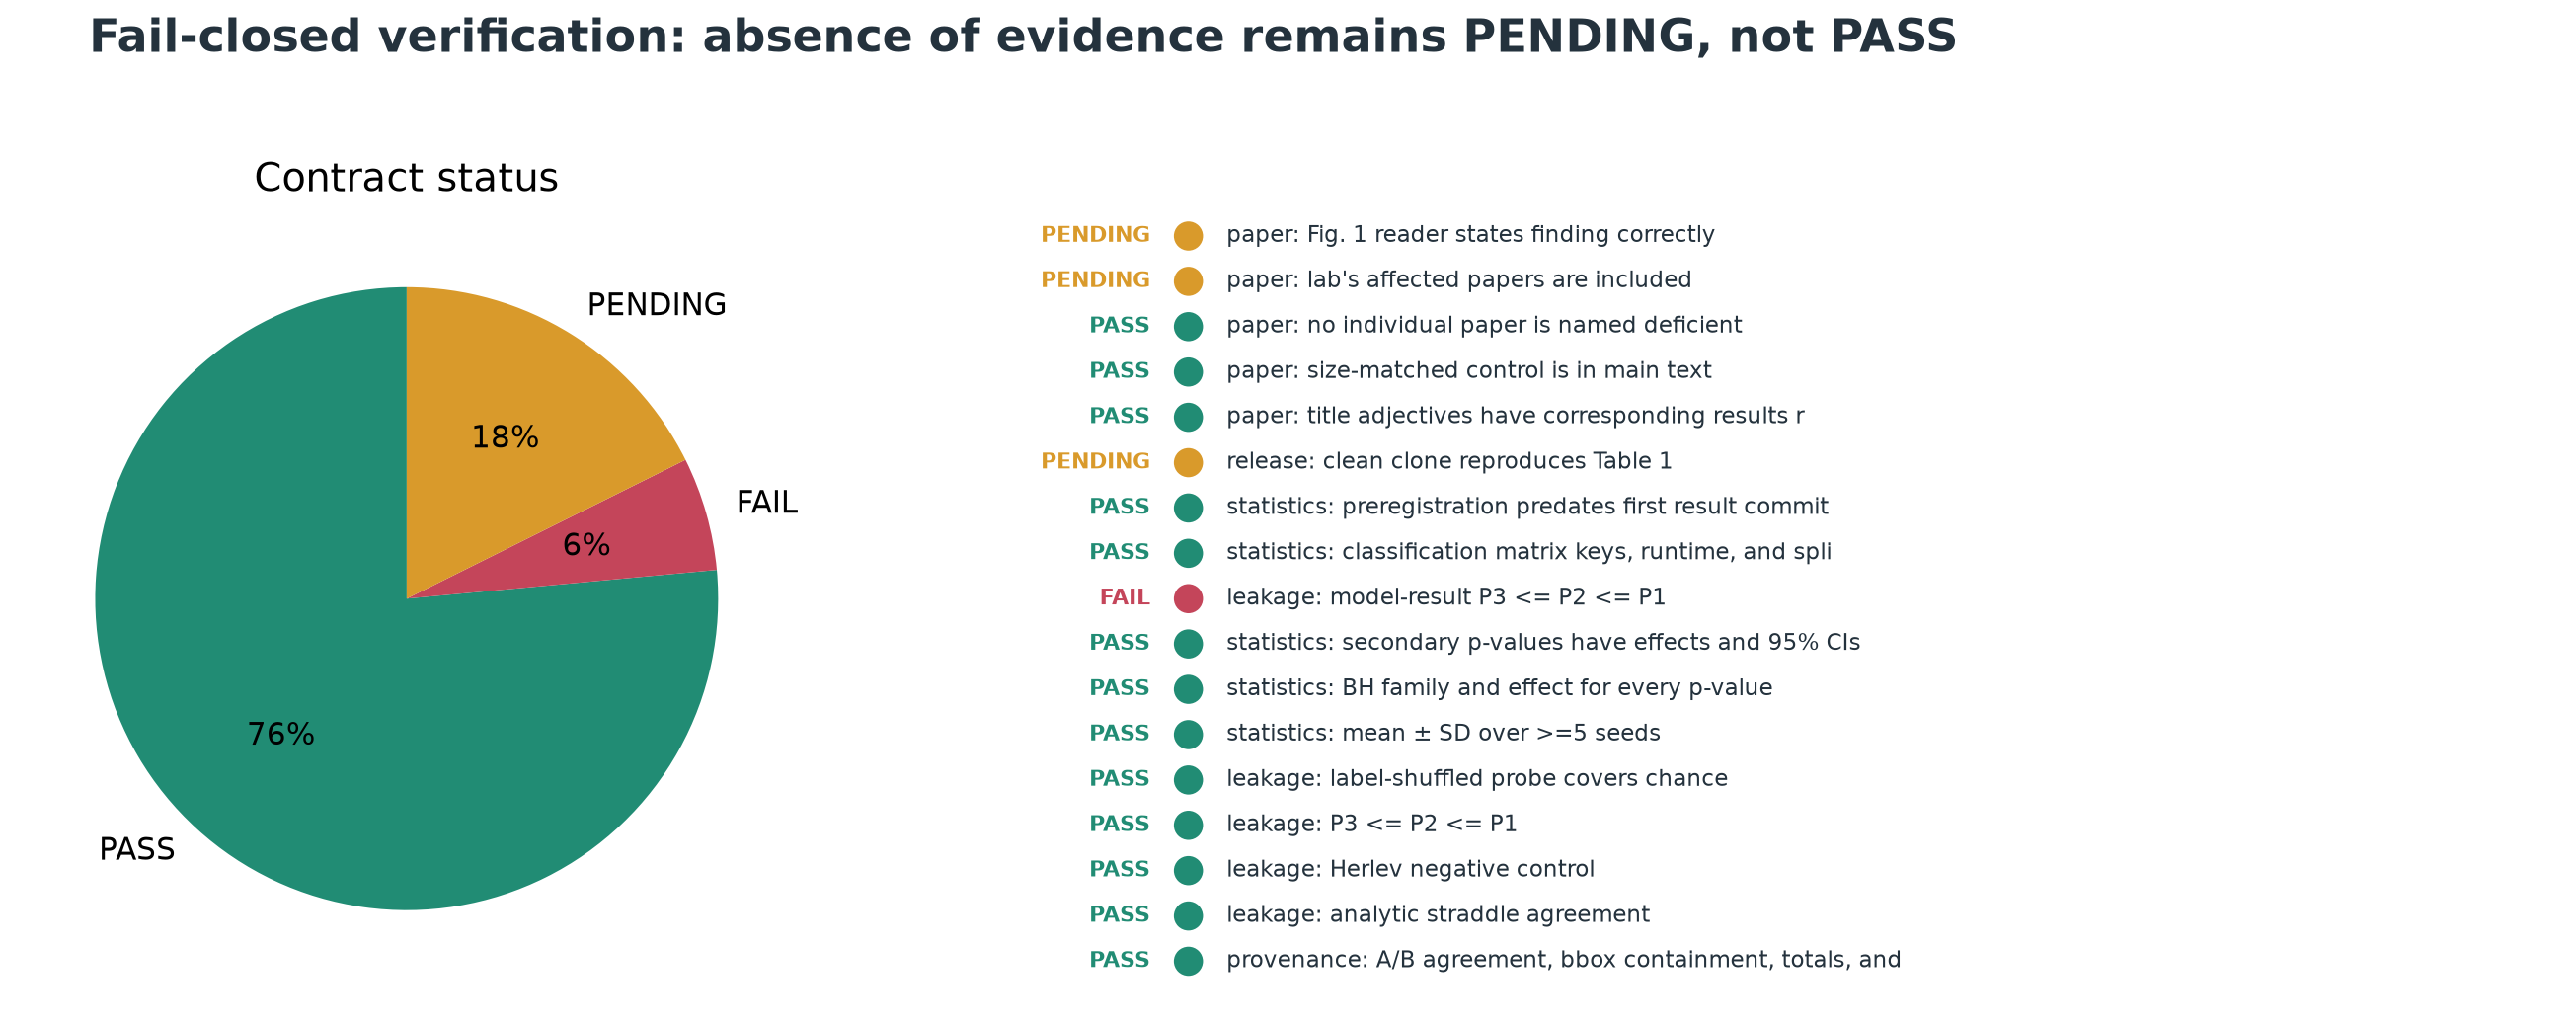
\includegraphics[width=\textwidth]{acceptance_dashboard.png}
\caption{Machine-readable acceptance status: 13 gates pass, one fails, and three remain pending. A pending release gate is not painted green simply because the numerical experiments are complete.}
\label{fig:acceptance}
\end{figure}

\begin{longtable}{p{0.29\textwidth}p{0.14\textwidth}p{0.45\textwidth}}
\caption{Acceptance contract with evidence.}
\label{tab:acceptance}\\
\toprule
Gate & Status & Evidence \\
\midrule
\endfirsthead
\toprule
Gate & Status & Evidence \\
\midrule
\endhead
\bottomrule
\endfoot
SIPaKMeD branch agreement $\geq99\%$ & \pass & 4,049/4,049 mappings agree (100\%). \\
Every bbox lies in parent bounds & \pass & 4,049/4,049 pass geometry checks. \\
Crop and per-class parent totals match & \pass & 4,049 crops; parent vector 126/108/238/271/223. \\
Observed straddle matches analytic prediction & \pass & All audited multi-crop datasets fall inside the recorded simulation envelope. \\
Herlev has no structural effect & \pass & All five seeds return exactly zero in \protocol{P1}; \protocol{P2}/\protocol{P3} also zero. \\
\protocol{P3}$\leq$\protocol{P2}$\leq$\protocol{P1}, structural & \pass & Grouped protocols eliminate measured parent sharing. \\
Shuffled probe confirms chance & \pass & 95\% $t$ interval [$-0.1385$, 0.4687]\% contains 0.2358\%. \\
Every neural summary has $\geq5$ seeds & \pass & 120 classifier, 30 probe, and 175 Cx22 files pass matrix completeness. \\
Plan predates first result commit & \pass & 22 Aug 2026 04:54:10 IST versus 13:22:42 IST. \\
BH applied over stated families & \pass & Stored family labels and $q$ values are reproduced from the exact supplied rows. \\
Effect accompanies every inferential $p$ & \pass & $d_z$, rank-biserial, or Kendall $\tau$ is present. \\
Classifier \protocol{P3}$\leq$\protocol{P2}$\leq$\protocol{P1} & \fail & Only ResNet-50 and ViT-B/16 pass; four of six fail. \\
Cx22 model ordering & \pass & All five semantic and two instance rows pass. \\
Official Cx22 parent disjointness & \pass & Multi-Train and Multi-Test have no shared recovered source parent. \\
Virgin-host clean-clone reproduction & \pending & Script exists, but execution evidence from a never-used host is absent. \\
Lab's own affected papers in audit & \pending & No verified crosswalk in the frozen repository. \\
Figure-1-only independent reader & \pending & No documented colleague response in the frozen repository. \\
\end{longtable}

\section{Why the classification ordering gate fails}

The structural ordering and model-score ordering are different propositions. \protocol{P3} has stricter grouping than \protocol{P2}, but it also creates a different balanced partition. Removing a small duplicate-connected component can alter class composition, parent difficulty, and which observations land in test. A finite test set can therefore score higher under the stricter split even though it contains less structural sharing. The failure warns against using monotonic score ordering as a definition of correctness; leakage absence should be checked directly from IDs and components.

\section{Release-readiness boundary}

The repository contains a one-script verification path, but the strongest release criterion requires a truly clean machine that has never held the repository or data. Running the script on the development host, even in a new directory, would not fully establish that environmental condition. This report therefore leaves the release gate pending. The same standard applies to the human communication gate and lab-paper crosswalk: absence of evidence is not converted into a pass.

\chapter{Interpretation, limitations, and practical guidance}

\section{What the evidence supports}

The source hierarchy is real and recoverable. Random crop splitting predictably separates siblings. In SIPaKMeD it can also put overlapping source pixels into training and test. Parent identity is learnable even after large parts of the apparent cell signal are removed. Parent- and component-disjoint protocols eliminate the directly measured sharing. These conclusions follow from deterministic identities, geometry, and controls, not from a single favorable neural score.

The downstream effect is subtler. Every tested \protocol{P1}$-$\protocol{P2} mean is positive, including six classifiers and seven segmentation models, but the Cx22 semantic differences are often tiny and none of the task-specific confirmatory families survives BH correction. The evidence supports changing split construction because independence is a design requirement, not because a guaranteed score penalty has been estimated.

\section{Two hard visual structures in Cx22}

The most persistent semantic error source is the nucleus channel. Nuclei occupy fewer pixels, so boundary uncertainty has a larger Dice penalty; pale nuclei and overlaps further reduce contrast. The second hard structure is touching cytoplasm instances. A union mask can remain visually plausible while an instance model merges two touching cells; maximum matching then assigns a good overlap to one target and zero or low overlap to the other. These explanations correspond to the actual label geometry in Figure~\ref{fig:cx22-labels} and the channel results in Figure~\ref{fig:cx22-channels}.

\section{Real limitations}

\begin{enumerate}[leftmargin=2em]
  \item \textbf{Dataset hierarchy stops at the released identifier.} SIPaKMeD fields and Cx22/CRIC sources are not guaranteed to be patient IDs. Parent-disjoint is therefore necessary but may not be sufficient for clinical independence.
  \item \textbf{Five seeds leave broad uncertainty.} The complete matrix is large in GPU hours but small in inferential replication. Shapiro screening and bootstrap effects are fragile at $n=5$.
  \item \textbf{No clinical validation.} The study audits public research benchmarks; it does not estimate screening sensitivity, specificity, prevalence calibration, reader impact, or deployment safety.
  \item \textbf{Hardware and host constraint.} Execution occurred on one login node with at most three A6000 GPUs and an unstable I/O bottleneck. Wall times are not portable performance claims.
  \item \textbf{Probe transformations are not surgical interventions.} Grayscale, normalization, inpainting, and high-pass filtering each alter multiple cues. They localize signal classes but do not identify a unique causal artifact.
  \item \textbf{Near-duplicate grouping is conservative and calibrated synthetically.} It found no exact cross-parent duplicates and validated candidate detection on 3 positive/100 negative synthetic examples, but it is not a proof that every biological near-duplicate was linked.
  \item \textbf{Prediction-level artifacts were not retained.} Post-hoc classifier confusion matrices and qualitative prediction panels cannot be reconstructed without new inference.
  \item \textbf{Reproduction remains pending on a virgin host.} Dependency or URL drift may still be exposed by that final test.
\end{enumerate}

\section{Recommended evaluation rule}

For any crop-derived cytology dataset, publish at least four fields for every released observation: a stable observation ID, an acquisition/source parent ID, a patient/specimen ID when ethically and legally possible, and a duplicate-component ID if cross-parent duplication was audited. Construct folds at the highest available independent level and publish the exact fold manifest. Report sample counts at both observation and parent levels. Never compare methods under nominally identical dataset names unless the split identifiers also match.

\section{What to say in a paper}

The defensible headline is: ``Random crop-level evaluation in public cervical cytology can place sibling and even pixel-overlapping crops across train and test; source-disjoint manifests remove this non-independence.'' A stronger sentence---``all published scores are inflated''---is not supported. No individual prior paper needs to be named as deficient; the target is a reusable benchmark practice.

\chapter{Reproduction and release engineering}

\section{From owner downloads to structural Table 1}

\begin{figure}[H]
\centering
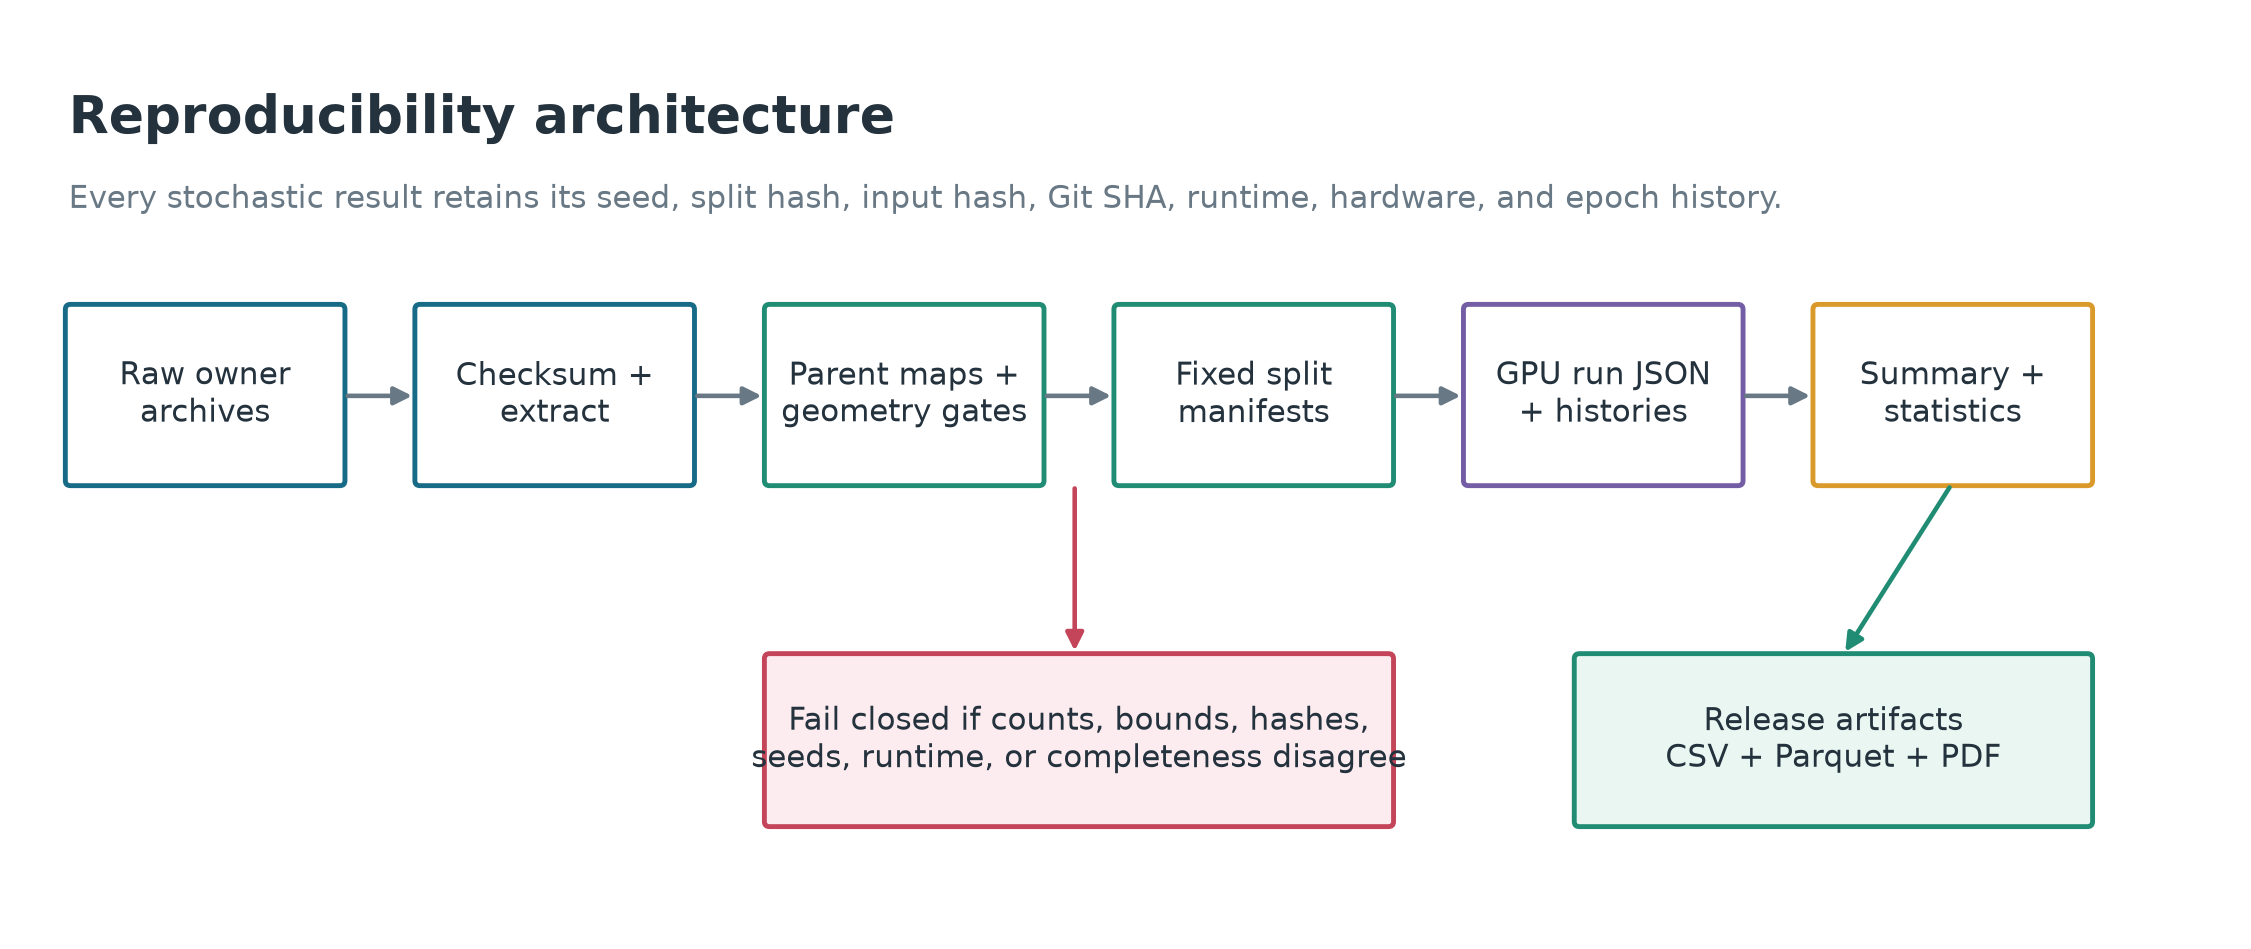
\includegraphics[width=\textwidth]{reproducibility_pipeline.png}
\caption{The intended clean-clone path. Each boundary writes an auditable artifact and performs validation before the next stage begins.}
\label{fig:reproduction}
\end{figure}

The GPU-free structural result has one public entry point:
\begin{lstlisting}[style=cyto,language=bash,caption={Raw-download-to-Table-1 entry point.}]
./scripts/reproduce_table1.sh
\end{lstlisting}
The script performs a locked dependency sync; downloads all declared owner files with at most three connections; verifies exact sizes and SHA-256 values; extracts archives; recovers SIPaKMeD, Cx22, CRIC, and Herlev provenance; runs the SIPaKMeD duplicate and pixel-overlap audits; creates fixed splits; and emits the dataset-level and seed-level structural tables.

Raw images are intentionally excluded from version control. The repository distributes URLs, checksums, IDs, coordinates, derived maps, split assignments, and results, subject to each source's terms. In particular, Cx22/CCEDD assets are non-commercial research resources and are not repackaged in this report.

\section{Clean-clone attestation}

The wrapper requires a repository URL and a destination that does not yet exist:
\begin{lstlisting}[style=cyto,language=bash,caption={Clean-clone verification wrapper.}]
./scripts/verify_clean_clone.sh \
  REPOSITORY_URL NEW_DESTINATION [GIT_REF]
\end{lstlisting}
It uses \artifact{git clone --no-local}, optionally checks out an exact detached ref, runs the reproduction script, and writes an attestation. A human/operator must set \artifact{CYTOFAIR_VIRGIN_HOST_ATTESTED=YES} only on a host that genuinely has never seen the project. The current repository lacks that final attested evidence, so release remains pending rather than assumed.

\section{Pinned software and result metadata}

The package requires Python 3.11 or newer. The result contract records NumPy 2.5.2, pandas 3.0.5, SciPy 1.18.1, scikit-learn 1.9.0, Pillow 12.3.0, OpenCV 5.0.0, PyTorch 2.9.0+cu128, torchvision 0.24.0+cu128, and CUDA 12.8 for the accepted classifier matrix. The lock file, not these prose values, is the install authority. The explicit versions remain useful diagnostics when a future lock update changes a hash.

\section{Atomicity and resumability}

Long GPU runs write checkpoints locally and copy them to a temporary destination name before atomic rename. A checkpoint is accepted only when its protocol, architecture, seed, and manifest hash match the requested cell. The launcher skips a result only after validating its completed JSON. A second launch can therefore resume interrupted work without accepting a mismatched or half-written file.

\section{Human-readable and machine-readable layers}

The project separates three layers:
\begin{itemize}
  \item \textbf{canonical data}: Parquet provenance maps and CSV split assignments;
  \item \textbf{machine evidence}: JSON run records, CSV summaries, hashes, and acceptance states;
  \item \textbf{human interpretation}: Markdown reports, figures, the conference paper, and this lifecycle monograph.
\end{itemize}
This prevents a narrative edit from changing the measured evidence and makes it possible to regenerate prose tables from structured files.

\chapter{Reusable outputs and future work}

\section{What exists now}

The most durable asset is not a new image collection. It is a stable interface between released observations and independent units: canonical parent maps, duplicate-component identifiers, fixed split CSVs, adjacent hashes, a leak-checking API, a run JSON schema, and paired statistics. A downstream model joins on \artifact{crop_id}; it never infers a split from row order or regenerates folds with a library default.

\section{Two publication units}

The conference unit is the complete provenance/leakage argument, mechanism probe, fixed split release, and matched SIPaKMeD rescore. A journal extension can add a separately preregistered annotation study, expanded cross-dataset validation, a broader detector ensemble, and power-oriented learning curves. These are partitioned future studies, not unreported parts of the present evidence.

\section{Projects unblocked}

\begin{table}[H]
\centering
\caption{Immediate technical reuse. These rows describe enabled work, not completed future experiments.}
\label{tab:reuse}
\begin{tabularx}{\textwidth}{lXX}
\toprule
Project & Reused asset & Work no longer rebuilt \\
\midrule
F3: Cx22 seed robustness & Parent map, fixed seeds, run schema, mean/SD and paired inference & Source grouping, seed ledger, rescore scaffold \\
F8: cross-dataset transfer & Canonical maps, split API, runtime metadata, label-crosswalk slot & Leakage-safe source folds and experiment provenance \\
F2: foundation encoders & P1/P1$'$/P2/P3 files and architecture-neutral summarizer & Fair split comparison, seed accounting, BH/effect reporting \\
\bottomrule
\end{tabularx}
\end{table}

\section{Pre-specified V2 in fish imagery}

Fish-Pak contains three views of the same specimen; Croatian Fish contains frames sampled at one frame per second from continuous BRUV/DOV video. The independent units become specimen and video episode. The planned V2 will: recover those units, compute analytic and observed frame straddling, construct specimen/episode-disjoint manifests, run the identity probe, and re-score fixed baselines under \protocol{P1}/\protocol{P1$'$}/\protocol{P2}/\protocol{P3}. No fish-domain result is claimed here.

\section{Adoption goal}

If versioned CytoFair manifests become the default evaluation interface, future papers can cite both the original dataset and the split asset while reporting exactly which parent-disjoint partition they used. This is an intended impact pathway, not a citation prediction or an empirical result.

\chapter{Conclusion}

This project asked whether a file-level train/test boundary corresponds to an independent acquisition boundary in public cervical cytology. It recovered and validated the hidden observation-to-parent hierarchy across four datasets, quantified the analytic and observed structural sharing, demonstrated literal source-pixel sharing in SIPaKMeD, and showed with a shuffled-label-controlled 424-way probe that parent identity remains strongly learnable after multiple cue-removal transformations. It then re-ran six classifiers and seven segmentation models over five fixed seeds and four matched protocols, preserving effect sizes, bootstrap intervals, multiplicity families, failures, and runtime metadata.

The strongest result is methodological: parent-disjoint evaluation is necessary whenever multiple released observations descend from one acquisition unit. The downstream neural results point in a consistent direction but do not justify a universal multiplicity-corrected accuracy-inflation claim. Four of six classifier architectures also violate the preregistered monotonic score ordering, a useful negative result showing that stricter grouping and lower finite-sample score are not synonymous.

CytoFair turns that lesson into reusable artifacts: provenance maps, duplicate components, fixed splits, hashes, fail-closed validators, run ledgers, and a raw-download structural pipeline. The next scientific step is a separately preregistered specimen/episode-disjoint fish-imagery V2; the next release step is a virgin-host clean-clone attestation. Until the latter, the numerical study is complete but the strongest release gate remains honestly pending.

\appendix

\chapter{Complete SIPaKMeD classifier run ledger}

The following 120 rows are the entire accepted classifier matrix. Accuracy, macro-F1, and balanced accuracy are final-epoch test values. This appendix makes every seed visible and prevents mean-only reporting from hiding an outlying run.

\begin{landscape}
\footnotesize
\setlength{\tabcolsep}{3pt}
\begin{longtable}{p{2.25cm}p{1.1cm}rrrrrrrr}
\caption{Complete SIPaKMeD classification run ledger. All values are final-epoch results.}\label{tab:all-class-runs}\\
\toprule
Architecture & Protocol & Seed & Train & Test & Acc. (percent) & Macro-F1 (percent) & Bal. acc. (percent) & min & GPU \\
\midrule
\endfirsthead
\toprule
Architecture & Protocol & Seed & Train & Test & Acc. (percent) & Macro-F1 (percent) & Bal. acc. (percent) & min & GPU \\
\midrule
\endhead
\bottomrule
\endfoot
densenet121 & P1 & 17 & 3239 & 810 & 98.519 & 98.521 & 98.527 & 4.66 & 3 \\ 
densenet121 & P1 & 29 & 3239 & 810 & 98.025 & 98.023 & 98.027 & 4.62 & 2 \\ 
densenet121 & P1 & 43 & 3239 & 810 & 97.778 & 97.776 & 97.803 & 4.54 & 1 \\ 
densenet121 & P1 & 71 & 3239 & 810 & 98.025 & 98.031 & 98.018 & 4.61 & 3 \\ 
densenet121 & P1 & 101 & 3239 & 810 & 98.272 & 98.284 & 98.276 & 4.70 & 2 \\ 
densenet121 & P1-prime & 17 & 3239 & 810 & 98.519 & 98.521 & 98.527 & 4.61 & 1 \\ 
densenet121 & P1-prime & 29 & 3239 & 810 & 98.025 & 98.023 & 98.027 & 4.48 & 3 \\ 
densenet121 & P1-prime & 43 & 3239 & 810 & 97.778 & 97.776 & 97.803 & 4.49 & 2 \\ 
densenet121 & P1-prime & 71 & 3239 & 810 & 98.025 & 98.031 & 98.018 & 4.48 & 1 \\ 
densenet121 & P1-prime & 101 & 3239 & 810 & 98.272 & 98.284 & 98.276 & 4.45 & 3 \\ 
densenet121 & P2 & 17 & 3239 & 810 & 95.926 & 95.972 & 95.946 & 4.47 & 2 \\ 
densenet121 & P2 & 29 & 3239 & 810 & 97.778 & 97.766 & 97.798 & 4.55 & 1 \\ 
densenet121 & P2 & 43 & 3239 & 810 & 96.914 & 96.927 & 96.906 & 4.51 & 3 \\ 
densenet121 & P2 & 71 & 3239 & 810 & 96.543 & 96.561 & 96.566 & 4.47 & 2 \\ 
densenet121 & P2 & 101 & 3239 & 810 & 96.420 & 96.446 & 96.395 & 4.59 & 1 \\ 
densenet121 & P3 & 17 & 3239 & 810 & 97.778 & 97.781 & 97.774 & 4.54 & 3 \\ 
densenet121 & P3 & 29 & 3239 & 810 & 97.901 & 97.895 & 97.904 & 4.64 & 2 \\ 
densenet121 & P3 & 43 & 3239 & 810 & 97.531 & 97.538 & 97.553 & 4.56 & 1 \\ 
densenet121 & P3 & 71 & 3239 & 810 & 96.790 & 96.824 & 96.801 & 4.20 & 3 \\ 
densenet121 & P3 & 101 & 3239 & 810 & 96.914 & 96.945 & 96.894 & 4.00 & 2 \\ 
efficientnet\_b0 & P1 & 17 & 3239 & 810 & 97.654 & 97.659 & 97.662 & 2.84 & 1 \\ 
efficientnet\_b0 & P1 & 29 & 3239 & 810 & 98.272 & 98.276 & 98.273 & 2.89 & 3 \\ 
efficientnet\_b0 & P1 & 43 & 3239 & 810 & 97.160 & 97.183 & 97.177 & 2.92 & 2 \\ 
efficientnet\_b0 & P1 & 71 & 3239 & 810 & 97.531 & 97.540 & 97.541 & 2.98 & 1 \\ 
efficientnet\_b0 & P1 & 101 & 3239 & 810 & 98.272 & 98.279 & 98.288 & 2.87 & 3 \\ 
efficientnet\_b0 & P1-prime & 17 & 3239 & 810 & 97.654 & 97.659 & 97.662 & 2.87 & 2 \\ 
efficientnet\_b0 & P1-prime & 29 & 3239 & 810 & 98.272 & 98.276 & 98.273 & 3.00 & 1 \\ 
efficientnet\_b0 & P1-prime & 43 & 3239 & 810 & 97.160 & 97.183 & 97.177 & 2.96 & 3 \\ 
efficientnet\_b0 & P1-prime & 71 & 3239 & 810 & 97.531 & 97.540 & 97.541 & 2.88 & 2 \\ 
efficientnet\_b0 & P1-prime & 101 & 3239 & 810 & 98.272 & 98.279 & 98.288 & 2.86 & 1 \\ 
efficientnet\_b0 & P2 & 17 & 3239 & 810 & 97.778 & 97.790 & 97.799 & 3.01 & 3 \\ 
efficientnet\_b0 & P2 & 29 & 3239 & 810 & 95.185 & 95.259 & 95.163 & 2.92 & 2 \\ 
efficientnet\_b0 & P2 & 43 & 3239 & 810 & 98.642 & 98.641 & 98.643 & 2.92 & 1 \\ 
efficientnet\_b0 & P2 & 71 & 3239 & 810 & 95.432 & 95.450 & 95.407 & 2.97 & 3 \\ 
efficientnet\_b0 & P2 & 101 & 3239 & 810 & 96.420 & 96.413 & 96.422 & 2.93 & 2 \\ 
efficientnet\_b0 & P3 & 17 & 3239 & 810 & 98.148 & 98.144 & 98.170 & 2.89 & 1 \\ 
efficientnet\_b0 & P3 & 29 & 3239 & 810 & 97.901 & 97.920 & 97.910 & 2.98 & 3 \\ 
efficientnet\_b0 & P3 & 43 & 3239 & 810 & 96.296 & 96.316 & 96.325 & 2.99 & 2 \\ 
efficientnet\_b0 & P3 & 71 & 3239 & 810 & 97.407 & 97.428 & 97.427 & 2.94 & 1 \\ 
efficientnet\_b0 & P3 & 101 & 3239 & 810 & 97.284 & 97.300 & 97.285 & 2.80 & 3 \\ 
mobilenet\_v2 & P1 & 17 & 3239 & 810 & 97.284 & 97.287 & 97.278 & 2.72 & 2 \\ 
mobilenet\_v2 & P1 & 29 & 3239 & 810 & 97.407 & 97.406 & 97.403 & 2.76 & 1 \\ 
mobilenet\_v2 & P1 & 43 & 3239 & 810 & 96.914 & 96.933 & 96.944 & 2.74 & 3 \\ 
mobilenet\_v2 & P1 & 71 & 3239 & 810 & 97.284 & 97.296 & 97.289 & 2.71 & 2 \\ 
mobilenet\_v2 & P1 & 101 & 3239 & 810 & 98.148 & 98.149 & 98.167 & 2.72 & 1 \\ 
mobilenet\_v2 & P1-prime & 17 & 3239 & 810 & 97.284 & 97.287 & 97.278 & 2.69 & 3 \\ 
mobilenet\_v2 & P1-prime & 29 & 3239 & 810 & 97.407 & 97.406 & 97.403 & 2.74 & 2 \\ 
mobilenet\_v2 & P1-prime & 43 & 3239 & 810 & 96.914 & 96.933 & 96.944 & 2.72 & 1 \\ 
mobilenet\_v2 & P1-prime & 71 & 3239 & 810 & 97.284 & 97.296 & 97.289 & 2.71 & 3 \\ 
mobilenet\_v2 & P1-prime & 101 & 3239 & 810 & 98.148 & 98.149 & 98.167 & 2.73 & 2 \\ 
mobilenet\_v2 & P2 & 17 & 3239 & 810 & 96.420 & 96.432 & 96.453 & 2.75 & 1 \\ 
mobilenet\_v2 & P2 & 29 & 3239 & 810 & 93.704 & 93.732 & 93.714 & 2.73 & 3 \\ 
mobilenet\_v2 & P2 & 43 & 3239 & 810 & 96.667 & 96.679 & 96.637 & 2.74 & 2 \\ 
mobilenet\_v2 & P2 & 71 & 3239 & 810 & 93.457 & 93.486 & 93.458 & 2.78 & 1 \\ 
mobilenet\_v2 & P2 & 101 & 3239 & 810 & 95.556 & 95.553 & 95.534 & 2.77 & 3 \\ 
mobilenet\_v2 & P3 & 17 & 3239 & 810 & 97.407 & 97.408 & 97.433 & 2.68 & 2 \\ 
mobilenet\_v2 & P3 & 29 & 3239 & 810 & 96.173 & 96.163 & 96.163 & 2.74 & 1 \\ 
mobilenet\_v2 & P3 & 43 & 3239 & 810 & 96.667 & 96.669 & 96.696 & 2.74 & 3 \\ 
mobilenet\_v2 & P3 & 71 & 3239 & 810 & 95.802 & 95.823 & 95.813 & 2.92 & 2 \\ 
mobilenet\_v2 & P3 & 101 & 3239 & 810 & 94.938 & 94.930 & 94.900 & 2.79 & 1 \\ 
resnet18 & P1 & 17 & 3239 & 810 & 97.901 & 97.900 & 97.930 & 2.57 & 1 \\ 
resnet18 & P1 & 29 & 3239 & 810 & 97.037 & 97.028 & 97.051 & 2.54 & 2 \\ 
resnet18 & P1 & 43 & 3239 & 810 & 96.914 & 96.922 & 96.938 & 2.48 & 3 \\ 
resnet18 & P1 & 71 & 3239 & 810 & 96.420 & 96.455 & 96.410 & 2.61 & 1 \\ 
resnet18 & P1 & 101 & 3239 & 810 & 97.654 & 97.661 & 97.674 & 2.54 & 2 \\ 
resnet18 & P1-prime & 17 & 3239 & 810 & 97.901 & 97.900 & 97.930 & 2.53 & 3 \\ 
resnet18 & P1-prime & 29 & 3239 & 810 & 97.037 & 97.028 & 97.051 & 2.62 & 1 \\ 
resnet18 & P1-prime & 43 & 3239 & 810 & 96.914 & 96.922 & 96.938 & 2.61 & 2 \\ 
resnet18 & P1-prime & 71 & 3239 & 810 & 96.420 & 96.455 & 96.410 & 2.48 & 3 \\ 
resnet18 & P1-prime & 101 & 3239 & 810 & 97.654 & 97.661 & 97.674 & 2.62 & 1 \\ 
resnet18 & P2 & 17 & 3239 & 810 & 96.420 & 96.444 & 96.447 & 2.58 & 2 \\ 
resnet18 & P2 & 29 & 3239 & 810 & 96.049 & 96.051 & 96.058 & 2.47 & 3 \\ 
resnet18 & P2 & 43 & 3239 & 810 & 96.543 & 96.535 & 96.502 & 2.49 & 1 \\ 
resnet18 & P2 & 71 & 3239 & 810 & 96.543 & 96.563 & 96.528 & 2.56 & 2 \\ 
resnet18 & P2 & 101 & 3239 & 810 & 94.444 & 94.436 & 94.384 & 2.50 & 3 \\ 
resnet18 & P3 & 17 & 3239 & 810 & 98.395 & 98.395 & 98.400 & 2.55 & 1 \\ 
resnet18 & P3 & 29 & 3239 & 810 & 95.062 & 95.069 & 95.014 & 2.55 & 3 \\ 
resnet18 & P3 & 43 & 3239 & 810 & 96.173 & 96.165 & 96.215 & 2.52 & 2 \\ 
resnet18 & P3 & 71 & 3239 & 810 & 96.543 & 96.578 & 96.561 & 2.79 & 1 \\ 
resnet18 & P3 & 101 & 3239 & 810 & 95.556 & 95.576 & 95.526 & 2.79 & 3 \\ 
resnet50 & P1 & 17 & 3239 & 810 & 97.778 & 97.781 & 97.792 & 3.73 & 2 \\ 
resnet50 & P1 & 29 & 3239 & 810 & 97.284 & 97.304 & 97.275 & 3.29 & 1 \\ 
resnet50 & P1 & 43 & 3239 & 810 & 96.790 & 96.801 & 96.805 & 3.32 & 3 \\ 
resnet50 & P1 & 71 & 3239 & 810 & 97.901 & 97.903 & 97.904 & 3.48 & 2 \\ 
resnet50 & P1 & 101 & 3239 & 810 & 97.778 & 97.776 & 97.777 & 3.45 & 1 \\ 
resnet50 & P1-prime & 17 & 3239 & 810 & 97.778 & 97.781 & 97.792 & 3.26 & 3 \\ 
resnet50 & P1-prime & 29 & 3239 & 810 & 97.284 & 97.304 & 97.275 & 3.45 & 2 \\ 
resnet50 & P1-prime & 43 & 3239 & 810 & 96.790 & 96.801 & 96.805 & 3.52 & 1 \\ 
resnet50 & P1-prime & 71 & 3239 & 810 & 97.901 & 97.903 & 97.904 & 3.34 & 3 \\ 
resnet50 & P1-prime & 101 & 3239 & 810 & 97.778 & 97.776 & 97.777 & 3.54 & 2 \\ 
resnet50 & P2 & 17 & 3239 & 810 & 97.037 & 97.067 & 97.053 & 3.47 & 1 \\ 
resnet50 & P2 & 29 & 3239 & 810 & 96.914 & 96.931 & 96.916 & 3.24 & 3 \\ 
resnet50 & P2 & 43 & 3239 & 810 & 97.284 & 97.298 & 97.290 & 3.45 & 2 \\ 
resnet50 & P2 & 71 & 3239 & 810 & 96.420 & 96.422 & 96.433 & 3.47 & 1 \\ 
resnet50 & P2 & 101 & 3239 & 810 & 96.296 & 96.303 & 96.288 & 3.29 & 3 \\ 
resnet50 & P3 & 17 & 3239 & 810 & 96.543 & 96.519 & 96.573 & 3.47 & 2 \\ 
resnet50 & P3 & 29 & 3239 & 810 & 97.037 & 97.071 & 97.049 & 3.46 & 1 \\ 
resnet50 & P3 & 43 & 3239 & 810 & 95.679 & 95.701 & 95.703 & 3.25 & 3 \\ 
resnet50 & P3 & 71 & 3239 & 810 & 95.926 & 95.945 & 95.958 & 3.73 & 2 \\ 
resnet50 & P3 & 101 & 3239 & 810 & 96.173 & 96.168 & 96.161 & 3.89 & 1 \\ 
vit\_b\_16 & P1 & 17 & 3239 & 810 & 97.407 & 97.414 & 97.430 & 9.30 & 3 \\ 
vit\_b\_16 & P1 & 29 & 3239 & 810 & 97.037 & 97.050 & 97.061 & 9.25 & 2 \\ 
vit\_b\_16 & P1 & 43 & 3239 & 810 & 95.556 & 95.541 & 95.606 & 9.35 & 1 \\ 
vit\_b\_16 & P1 & 71 & 3239 & 810 & 98.025 & 98.036 & 98.023 & 9.31 & 3 \\ 
vit\_b\_16 & P1 & 101 & 3239 & 810 & 97.654 & 97.666 & 97.684 & 9.27 & 2 \\ 
vit\_b\_16 & P1-prime & 17 & 3239 & 810 & 97.407 & 97.414 & 97.430 & 9.29 & 1 \\ 
vit\_b\_16 & P1-prime & 29 & 3239 & 810 & 97.037 & 97.050 & 97.061 & 9.19 & 3 \\ 
vit\_b\_16 & P1-prime & 43 & 3239 & 810 & 95.556 & 95.541 & 95.606 & 9.24 & 2 \\ 
vit\_b\_16 & P1-prime & 71 & 3239 & 810 & 98.025 & 98.036 & 98.023 & 9.30 & 1 \\ 
vit\_b\_16 & P1-prime & 101 & 3239 & 810 & 97.654 & 97.666 & 97.684 & 9.24 & 3 \\ 
vit\_b\_16 & P2 & 17 & 3239 & 810 & 95.556 & 95.618 & 95.526 & 9.27 & 2 \\ 
vit\_b\_16 & P2 & 29 & 3239 & 810 & 95.802 & 95.821 & 95.788 & 9.36 & 1 \\ 
vit\_b\_16 & P2 & 43 & 3239 & 810 & 96.667 & 96.693 & 96.688 & 9.32 & 3 \\ 
vit\_b\_16 & P2 & 71 & 3239 & 810 & 95.432 & 95.432 & 95.392 & 9.30 & 2 \\ 
vit\_b\_16 & P2 & 101 & 3239 & 810 & 94.321 & 94.421 & 94.283 & 9.28 & 1 \\ 
vit\_b\_16 & P3 & 17 & 3239 & 810 & 96.296 & 96.258 & 96.328 & 9.19 & 3 \\ 
vit\_b\_16 & P3 & 29 & 3239 & 810 & 95.185 & 95.218 & 95.214 & 9.23 & 2 \\ 
vit\_b\_16 & P3 & 43 & 3239 & 810 & 92.840 & 92.915 & 92.770 & 9.26 & 1 \\ 
vit\_b\_16 & P3 & 71 & 3239 & 810 & 97.284 & 97.292 & 97.301 & 9.00 & 3 \\ 
vit\_b\_16 & P3 & 101 & 3239 & 810 & 96.049 & 96.039 & 96.066 & 8.81 & 2 \\ 
\end{longtable}

\end{landscape}

\chapter{Complete parent-probe run ledger}

These 30 rows include five preprocessing arms and the label-shuffled negative control. All use exactly 424 parent classes, 848 training crops, and 848 held-out sibling crops.

\begin{landscape}
\footnotesize
\setlength{\tabcolsep}{3pt}
\begin{longtable}{p{2.4cm}p{1.0cm}rrrrrrrr}
\caption{Complete parent-identity probe ledger.}\label{tab:all-probe-runs}\\
\toprule
Mode & Shuffle & Seed & Parents & Train & Test & Chance (percent) & Accuracy (percent) & min & GPU \\
\midrule
\endfirsthead
\toprule
Mode & Shuffle & Seed & Parents & Train & Test & Chance (percent) & Accuracy (percent) & min & GPU \\
\midrule
\endhead
\bottomrule
\endfoot
background\_only & no & 17 & 424 & 848 & 848 & 0.2358 & 18.514 & 21.00 & 3 \\ 
background\_only & no & 29 & 424 & 848 & 848 & 0.2358 & 20.047 & 20.55 & 1 \\ 
background\_only & no & 43 & 424 & 848 & 848 & 0.2358 & 19.811 & 20.23 & 2 \\ 
background\_only & no & 71 & 424 & 848 & 848 & 0.2358 & 17.925 & 89.59 & 3 \\ 
background\_only & no & 101 & 424 & 848 & 848 & 0.2358 & 17.099 & 89.40 & 2 \\ 
grayscale & no & 17 & 424 & 848 & 848 & 0.2358 & 15.212 & 0.93 & 3 \\ 
grayscale & no & 29 & 424 & 848 & 848 & 0.2358 & 13.208 & 0.88 & 2 \\ 
grayscale & no & 43 & 424 & 848 & 848 & 0.2358 & 14.741 & 1.02 & 1 \\ 
grayscale & no & 71 & 424 & 848 & 848 & 0.2358 & 13.208 & 0.97 & 2 \\ 
grayscale & no & 101 & 424 & 848 & 848 & 0.2358 & 12.618 & 1.02 & 3 \\ 
highpass & no & 17 & 424 & 848 & 848 & 0.2358 & 16.863 & 15.73 & 1 \\ 
highpass & no & 29 & 424 & 848 & 848 & 0.2358 & 16.156 & 15.87 & 1 \\ 
highpass & no & 43 & 424 & 848 & 848 & 0.2358 & 16.863 & 15.93 & 1 \\ 
highpass & no & 71 & 424 & 848 & 848 & 0.2358 & 16.038 & 15.80 & 1 \\ 
highpass & no & 101 & 424 & 848 & 848 & 0.2358 & 15.448 & 16.04 & 1 \\ 
rgb & no & 17 & 424 & 848 & 848 & 0.2358 & 25.943 & 0.89 & 1 \\ 
rgb & no & 29 & 424 & 848 & 848 & 0.2358 & 26.769 & 0.76 & 2 \\ 
rgb & no & 43 & 424 & 848 & 848 & 0.2358 & 25.236 & 0.76 & 3 \\ 
rgb & no & 71 & 424 & 848 & 848 & 0.2358 & 25.590 & 0.77 & 1 \\ 
rgb & no & 101 & 424 & 848 & 848 & 0.2358 & 25.118 & 0.79 & 2 \\ 
rgb & yes & 17 & 424 & 848 & 848 & 0.2358 & 0.590 & 0.78 & 3 \\ 
rgb & yes & 29 & 424 & 848 & 848 & 0.2358 & 0.000 & 0.88 & 1 \\ 
rgb & yes & 43 & 424 & 848 & 848 & 0.2358 & 0.118 & 0.86 & 3 \\ 
rgb & yes & 71 & 424 & 848 & 848 & 0.2358 & 0.000 & 0.76 & 2 \\ 
rgb & yes & 101 & 424 & 848 & 848 & 0.2358 & 0.118 & 0.82 & 1 \\ 
stain\_normalized & no & 17 & 424 & 848 & 848 & 0.2358 & 17.335 & 2.49 & 1 \\ 
stain\_normalized & no & 29 & 424 & 848 & 848 & 0.2358 & 17.099 & 2.41 & 2 \\ 
stain\_normalized & no & 43 & 424 & 848 & 848 & 0.2358 & 18.396 & 2.26 & 3 \\ 
stain\_normalized & no & 71 & 424 & 848 & 848 & 0.2358 & 16.745 & 2.42 & 1 \\ 
stain\_normalized & no & 101 & 424 & 848 & 848 & 0.2358 & 16.981 & 2.20 & 2 \\ 
\end{longtable}

\end{landscape}

\chapter{Complete Cx22 model run ledger}

The following 175 rows are all accepted Cx22 cells: five semantic architectures and two instance architectures, each under five protocols and five seeds. ``Primary'' is semantic macro-Dice or matched-instance Dice; ``Nuc./R70'' is nucleus Dice for semantic rows and Recall@0.70 for instance rows.

\begin{landscape}
\scriptsize
\setlength{\tabcolsep}{2.2pt}
\begin{longtable}{p{1.6cm}p{4.4cm}p{1.5cm}rrrrrrr}
\caption{Complete Cx22 run ledger. Primary is macro Dice for semantic models and matched-instance Dice for instance models; the ninth column is nucleus Dice or recall at Dice 0.70.}\label{tab:all-cx22-runs}\\
\toprule
Task & Architecture & Protocol & Seed & Train & Test & Primary (percent) & IoU (percent) & Nuc./R70 (percent) & hours \\
\midrule
\endfirsthead
\toprule
Task & Architecture & Protocol & Seed & Train & Test & Primary (percent) & IoU (percent) & Nuc./R70 (percent) & hours \\
\midrule
\endhead
\bottomrule
\endfoot
instance & \path{maskrcnn_resnet50_fpn} & OFFICIAL & 17 & 400 & 100 & 92.117 & 87.060 & 96.991 & 14.35 \\ 
instance & \path{maskrcnn_resnet50_fpn} & OFFICIAL & 29 & 400 & 100 & 92.372 & 87.354 & 97.068 & 14.92 \\ 
instance & \path{maskrcnn_resnet50_fpn} & OFFICIAL & 43 & 400 & 100 & 91.844 & 86.861 & 96.682 & 15.89 \\ 
instance & \path{maskrcnn_resnet50_fpn} & OFFICIAL & 71 & 400 & 100 & 92.669 & 87.541 & 97.608 & 0.49 \\ 
instance & \path{maskrcnn_resnet50_fpn} & OFFICIAL & 101 & 400 & 100 & 92.433 & 87.559 & 97.145 & 1.29 \\ 
instance & \path{maskrcnn_resnet50_fpn} & P1 & 17 & 1056 & 264 & 92.683 & 87.370 & 96.540 & 33.85 \\ 
instance & \path{maskrcnn_resnet50_fpn} & P1 & 29 & 1056 & 264 & 91.354 & 86.327 & 95.009 & 33.71 \\ 
instance & \path{maskrcnn_resnet50_fpn} & P1 & 43 & 1056 & 264 & 92.282 & 87.191 & 96.854 & 35.84 \\ 
instance & \path{maskrcnn_resnet50_fpn} & P1 & 71 & 1056 & 264 & 92.343 & 87.320 & 96.550 & 37.54 \\ 
instance & \path{maskrcnn_resnet50_fpn} & P1 & 101 & 1056 & 264 & 91.819 & 86.735 & 96.471 & 2.55 \\ 
instance & \path{maskrcnn_resnet50_fpn} & P1-prime & 17 & 1056 & 264 & 92.683 & 87.370 & 96.540 & 33.94 \\ 
instance & \path{maskrcnn_resnet50_fpn} & P1-prime & 29 & 1056 & 264 & 91.354 & 86.327 & 95.009 & 33.95 \\ 
instance & \path{maskrcnn_resnet50_fpn} & P1-prime & 43 & 1056 & 264 & 92.282 & 87.191 & 96.854 & 35.19 \\ 
instance & \path{maskrcnn_resnet50_fpn} & P1-prime & 71 & 1055 & 264 & 91.733 & 86.958 & 95.483 & 38.29 \\ 
instance & \path{maskrcnn_resnet50_fpn} & P1-prime & 101 & 1053 & 264 & 92.213 & 87.257 & 97.248 & 2.56 \\ 
instance & \path{maskrcnn_resnet50_fpn} & P2 & 17 & 1056 & 264 & 91.815 & 86.503 & 95.983 & 33.84 \\ 
instance & \path{maskrcnn_resnet50_fpn} & P2 & 29 & 1056 & 264 & 91.313 & 86.228 & 95.159 & 34.29 \\ 
instance & \path{maskrcnn_resnet50_fpn} & P2 & 43 & 1056 & 264 & 92.024 & 86.559 & 96.750 & 35.88 \\ 
instance & \path{maskrcnn_resnet50_fpn} & P2 & 71 & 1055 & 265 & 90.993 & 85.998 & 92.239 & 0.26 \\ 
instance & \path{maskrcnn_resnet50_fpn} & P2 & 101 & 1053 & 267 & 91.793 & 86.639 & 94.671 & 2.57 \\ 
instance & \path{maskrcnn_resnet50_fpn} & P3 & 17 & 891 & 429 & 89.855 & 84.435 & 94.937 & 47.44 \\ 
instance & \path{maskrcnn_resnet50_fpn} & P3 & 29 & 825 & 495 & 91.606 & 86.357 & 95.207 & 49.79 \\ 
instance & \path{maskrcnn_resnet50_fpn} & P3 & 43 & 894 & 426 & 90.023 & 84.807 & 94.415 & 47.25 \\ 
instance & \path{maskrcnn_resnet50_fpn} & P3 & 71 & 773 & 547 & 92.181 & 86.751 & 96.205 & 1.16 \\ 
instance & \path{maskrcnn_resnet50_fpn} & P3 & 101 & 791 & 529 & 91.910 & 86.399 & 96.806 & 1.98 \\ 
instance & \path{maskrcnn_resnet50_fpn_v2} & OFFICIAL & 17 & 400 & 100 & 91.970 & 87.274 & 95.910 & 1.31 \\ 
instance & \path{maskrcnn_resnet50_fpn_v2} & OFFICIAL & 29 & 400 & 100 & 92.548 & 87.588 & 96.991 & 1.33 \\ 
instance & \path{maskrcnn_resnet50_fpn_v2} & OFFICIAL & 43 & 400 & 100 & 91.041 & 86.290 & 94.367 & 1.32 \\ 
instance & \path{maskrcnn_resnet50_fpn_v2} & OFFICIAL & 71 & 400 & 100 & 92.442 & 87.459 & 97.068 & 1.69 \\ 
instance & \path{maskrcnn_resnet50_fpn_v2} & OFFICIAL & 101 & 400 & 100 & 92.886 & 87.943 & 97.531 & 1.40 \\ 
instance & \path{maskrcnn_resnet50_fpn_v2} & P1 & 17 & 1056 & 264 & 91.235 & 86.322 & 91.816 & 2.63 \\ 
instance & \path{maskrcnn_resnet50_fpn_v2} & P1 & 29 & 1056 & 264 & 91.543 & 86.726 & 92.276 & 2.64 \\ 
instance & \path{maskrcnn_resnet50_fpn_v2} & P1 & 43 & 1056 & 264 & 92.536 & 87.688 & 94.870 & 2.65 \\ 
instance & \path{maskrcnn_resnet50_fpn_v2} & P1 & 71 & 1056 & 264 & 92.342 & 87.566 & 94.856 & 2.63 \\ 
instance & \path{maskrcnn_resnet50_fpn_v2} & P1 & 101 & 1056 & 264 & 92.318 & 87.546 & 95.131 & 2.99 \\ 
instance & \path{maskrcnn_resnet50_fpn_v2} & P1-prime & 17 & 1056 & 264 & 91.235 & 86.322 & 91.816 & 2.63 \\ 
instance & \path{maskrcnn_resnet50_fpn_v2} & P1-prime & 29 & 1056 & 264 & 91.543 & 86.726 & 92.276 & 2.63 \\ 
instance & \path{maskrcnn_resnet50_fpn_v2} & P1-prime & 43 & 1056 & 264 & 92.536 & 87.688 & 94.870 & 2.64 \\ 
instance & \path{maskrcnn_resnet50_fpn_v2} & P1-prime & 71 & 1055 & 264 & 91.938 & 87.241 & 93.915 & 2.62 \\ 
instance & \path{maskrcnn_resnet50_fpn_v2} & P1-prime & 101 & 1053 & 264 & 92.502 & 87.584 & 95.272 & 2.85 \\ 
instance & \path{maskrcnn_resnet50_fpn_v2} & P2 & 17 & 1056 & 264 & 92.036 & 87.121 & 95.303 & 2.64 \\ 
instance & \path{maskrcnn_resnet50_fpn_v2} & P2 & 29 & 1056 & 264 & 91.737 & 86.754 & 94.870 & 2.65 \\ 
instance & \path{maskrcnn_resnet50_fpn_v2} & P2 & 43 & 1056 & 264 & 92.056 & 86.980 & 95.297 & 2.65 \\ 
instance & \path{maskrcnn_resnet50_fpn_v2} & P2 & 71 & 1055 & 265 & 90.232 & 85.363 & 87.492 & 2.64 \\ 
instance & \path{maskrcnn_resnet50_fpn_v2} & P2 & 101 & 1053 & 267 & 90.762 & 85.672 & 92.038 & 2.70 \\ 
instance & \path{maskrcnn_resnet50_fpn_v2} & P3 & 17 & 891 & 429 & 91.242 & 85.867 & 94.762 & 2.26 \\ 
instance & \path{maskrcnn_resnet50_fpn_v2} & P3 & 29 & 825 & 495 & 89.960 & 84.956 & 91.273 & 2.10 \\ 
instance & \path{maskrcnn_resnet50_fpn_v2} & P3 & 43 & 894 & 426 & 90.317 & 85.094 & 91.622 & 2.29 \\ 
instance & \path{maskrcnn_resnet50_fpn_v2} & P3 & 71 & 773 & 547 & 90.474 & 85.440 & 90.769 & 1.98 \\ 
instance & \path{maskrcnn_resnet50_fpn_v2} & P3 & 101 & 791 & 529 & 91.026 & 85.770 & 94.358 & 2.02 \\ 
semantic & \path{deeplabv3plus_resnet50} & OFFICIAL & 17 & 400 & 100 & 82.697 & 72.771 & 71.084 & 1.02 \\ 
semantic & \path{deeplabv3plus_resnet50} & OFFICIAL & 29 & 400 & 100 & 83.602 & 73.897 & 72.700 & 1.13 \\ 
semantic & \path{deeplabv3plus_resnet50} & OFFICIAL & 43 & 400 & 100 & 84.126 & 74.580 & 73.775 & 1.08 \\ 
semantic & \path{deeplabv3plus_resnet50} & OFFICIAL & 71 & 400 & 100 & 83.972 & 74.385 & 73.418 & 1.12 \\ 
semantic & \path{deeplabv3plus_resnet50} & OFFICIAL & 101 & 400 & 100 & 80.382 & 70.180 & 66.995 & 1.11 \\ 
semantic & \path{deeplabv3plus_resnet50} & P1 & 17 & 1056 & 264 & 88.570 & 80.909 & 81.412 & 2.09 \\ 
semantic & \path{deeplabv3plus_resnet50} & P1 & 29 & 1056 & 264 & 88.464 & 80.728 & 81.373 & 1.91 \\ 
semantic & \path{deeplabv3plus_resnet50} & P1 & 43 & 1056 & 264 & 89.196 & 81.695 & 82.572 & 2.02 \\ 
semantic & \path{deeplabv3plus_resnet50} & P1 & 71 & 1056 & 264 & 89.542 & 82.165 & 83.162 & 2.14 \\ 
semantic & \path{deeplabv3plus_resnet50} & P1 & 101 & 1056 & 264 & 88.738 & 81.195 & 81.662 & 2.32 \\ 
semantic & \path{deeplabv3plus_resnet50} & P1-prime & 17 & 1056 & 264 & 88.570 & 80.909 & 81.412 & 2.13 \\ 
semantic & \path{deeplabv3plus_resnet50} & P1-prime & 29 & 1056 & 264 & 88.464 & 80.728 & 81.373 & 1.93 \\ 
semantic & \path{deeplabv3plus_resnet50} & P1-prime & 43 & 1056 & 264 & 89.196 & 81.695 & 82.572 & 2.03 \\ 
semantic & \path{deeplabv3plus_resnet50} & P1-prime & 71 & 1055 & 264 & 89.443 & 82.040 & 82.958 & 2.14 \\ 
semantic & \path{deeplabv3plus_resnet50} & P1-prime & 101 & 1053 & 264 & 88.514 & 80.848 & 81.162 & 2.28 \\ 
semantic & \path{deeplabv3plus_resnet50} & P2 & 17 & 1056 & 264 & 88.304 & 80.549 & 81.070 & 1.90 \\ 
semantic & \path{deeplabv3plus_resnet50} & P2 & 29 & 1056 & 264 & 88.930 & 81.407 & 82.016 & 2.03 \\ 
semantic & \path{deeplabv3plus_resnet50} & P2 & 43 & 1056 & 264 & 88.731 & 80.967 & 81.799 & 1.99 \\ 
semantic & \path{deeplabv3plus_resnet50} & P2 & 71 & 1055 & 265 & 88.988 & 81.513 & 82.202 & 2.22 \\ 
semantic & \path{deeplabv3plus_resnet50} & P2 & 101 & 1053 & 267 & 88.268 & 80.470 & 80.952 & 2.28 \\ 
semantic & \path{deeplabv3plus_resnet50} & P3 & 17 & 891 & 429 & 88.332 & 80.528 & 81.111 & 2.13 \\ 
semantic & \path{deeplabv3plus_resnet50} & P3 & 29 & 825 & 495 & 87.707 & 79.682 & 80.088 & 2.57 \\ 
semantic & \path{deeplabv3plus_resnet50} & P3 & 43 & 894 & 426 & 88.621 & 80.940 & 81.705 & 2.70 \\ 
semantic & \path{deeplabv3plus_resnet50} & P3 & 71 & 773 & 547 & 88.041 & 80.050 & 80.594 & 3.46 \\ 
semantic & \path{deeplabv3plus_resnet50} & P3 & 101 & 791 & 529 & 87.790 & 79.677 & 80.185 & 3.43 \\ 
semantic & \path{fpn_resnet34} & OFFICIAL & 17 & 400 & 100 & 84.378 & 74.779 & 74.746 & 1.08 \\ 
semantic & \path{fpn_resnet34} & OFFICIAL & 29 & 400 & 100 & 84.801 & 75.377 & 75.422 & 1.12 \\ 
semantic & \path{fpn_resnet34} & OFFICIAL & 43 & 400 & 100 & 84.389 & 74.760 & 74.723 & 1.10 \\ 
semantic & \path{fpn_resnet34} & OFFICIAL & 71 & 400 & 100 & 84.630 & 75.136 & 75.152 & 1.07 \\ 
semantic & \path{fpn_resnet34} & OFFICIAL & 101 & 400 & 100 & 83.934 & 74.231 & 73.850 & 1.09 \\ 
semantic & \path{fpn_resnet34} & P1 & 17 & 1056 & 264 & 88.606 & 80.936 & 81.657 & 2.30 \\ 
semantic & \path{fpn_resnet34} & P1 & 29 & 1056 & 264 & 88.376 & 80.651 & 81.204 & 2.17 \\ 
semantic & \path{fpn_resnet34} & P1 & 43 & 1056 & 264 & 89.242 & 81.731 & 82.802 & 2.29 \\ 
semantic & \path{fpn_resnet34} & P1 & 71 & 1056 & 264 & 89.415 & 81.991 & 83.139 & 2.29 \\ 
semantic & \path{fpn_resnet34} & P1 & 101 & 1056 & 264 & 88.854 & 81.286 & 81.903 & 2.31 \\ 
semantic & \path{fpn_resnet34} & P1-prime & 17 & 1056 & 264 & 88.606 & 80.936 & 81.657 & 2.23 \\ 
semantic & \path{fpn_resnet34} & P1-prime & 29 & 1056 & 264 & 88.376 & 80.651 & 81.204 & 2.19 \\ 
semantic & \path{fpn_resnet34} & P1-prime & 43 & 1056 & 264 & 89.242 & 81.731 & 82.802 & 2.30 \\ 
semantic & \path{fpn_resnet34} & P1-prime & 71 & 1055 & 264 & 89.760 & 82.473 & 83.695 & 2.30 \\ 
semantic & \path{fpn_resnet34} & P1-prime & 101 & 1053 & 264 & 88.880 & 81.350 & 81.891 & 2.26 \\ 
semantic & \path{fpn_resnet34} & P2 & 17 & 1056 & 264 & 88.539 & 80.901 & 81.452 & 2.18 \\ 
semantic & \path{fpn_resnet34} & P2 & 29 & 1056 & 264 & 89.006 & 81.470 & 82.385 & 2.20 \\ 
semantic & \path{fpn_resnet34} & P2 & 43 & 1056 & 264 & 89.498 & 82.080 & 83.321 & 2.22 \\ 
semantic & \path{fpn_resnet34} & P2 & 71 & 1055 & 265 & 89.102 & 81.618 & 82.649 & 2.24 \\ 
semantic & \path{fpn_resnet34} & P2 & 101 & 1053 & 267 & 88.296 & 80.471 & 81.211 & 2.25 \\ 
semantic & \path{fpn_resnet34} & P3 & 17 & 891 & 429 & 88.029 & 80.133 & 80.698 & 2.84 \\ 
semantic & \path{fpn_resnet34} & P3 & 29 & 825 & 495 & 88.080 & 80.127 & 80.967 & 3.16 \\ 
semantic & \path{fpn_resnet34} & P3 & 43 & 894 & 426 & 88.744 & 81.048 & 82.174 & 2.75 \\ 
semantic & \path{fpn_resnet34} & P3 & 71 & 773 & 547 & 88.510 & 80.711 & 81.583 & 3.46 \\ 
semantic & \path{fpn_resnet34} & P3 & 101 & 791 & 529 & 88.287 & 80.367 & 81.266 & 3.45 \\ 
semantic & \path{manet_resnet34} & OFFICIAL & 17 & 400 & 100 & 83.189 & 73.517 & 71.864 & 1.06 \\ 
semantic & \path{manet_resnet34} & OFFICIAL & 29 & 400 & 100 & 86.409 & 77.571 & 77.856 & 1.08 \\ 
semantic & \path{manet_resnet34} & OFFICIAL & 43 & 400 & 100 & 86.521 & 77.608 & 78.266 & 1.07 \\ 
semantic & \path{manet_resnet34} & OFFICIAL & 71 & 400 & 100 & 86.256 & 77.306 & 77.825 & 1.15 \\ 
semantic & \path{manet_resnet34} & OFFICIAL & 101 & 400 & 100 & 85.118 & 75.878 & 75.519 & 1.19 \\ 
semantic & \path{manet_resnet34} & P1 & 17 & 1056 & 264 & 89.317 & 81.998 & 82.837 & 2.13 \\ 
semantic & \path{manet_resnet34} & P1 & 29 & 1056 & 264 & 89.510 & 82.294 & 83.125 & 2.19 \\ 
semantic & \path{manet_resnet34} & P1 & 43 & 1056 & 264 & 90.535 & 83.620 & 85.003 & 2.09 \\ 
semantic & \path{manet_resnet34} & P1 & 71 & 1056 & 264 & 90.674 & 83.752 & 85.088 & 2.06 \\ 
semantic & \path{manet_resnet34} & P1 & 101 & 1056 & 264 & 90.128 & 83.049 & 84.158 & 2.14 \\ 
semantic & \path{manet_resnet34} & P1-prime & 17 & 1056 & 264 & 89.317 & 81.998 & 82.837 & 2.17 \\ 
semantic & \path{manet_resnet34} & P1-prime & 29 & 1056 & 264 & 89.510 & 82.294 & 83.125 & 2.06 \\ 
semantic & \path{manet_resnet34} & P1-prime & 43 & 1056 & 264 & 90.535 & 83.620 & 85.003 & 2.05 \\ 
semantic & \path{manet_resnet34} & P1-prime & 71 & 1055 & 264 & 90.764 & 83.957 & 85.467 & 2.05 \\ 
semantic & \path{manet_resnet34} & P1-prime & 101 & 1053 & 264 & 90.221 & 83.230 & 84.212 & 2.07 \\ 
semantic & \path{manet_resnet34} & P2 & 17 & 1056 & 264 & 89.337 & 81.962 & 83.086 & 2.14 \\ 
semantic & \path{manet_resnet34} & P2 & 29 & 1056 & 264 & 90.185 & 83.160 & 84.409 & 2.08 \\ 
semantic & \path{manet_resnet34} & P2 & 43 & 1056 & 264 & 90.170 & 83.032 & 84.460 & 2.01 \\ 
semantic & \path{manet_resnet34} & P2 & 71 & 1055 & 265 & 90.458 & 83.608 & 84.919 & 2.09 \\ 
semantic & \path{manet_resnet34} & P2 & 101 & 1053 & 267 & 89.687 & 82.410 & 83.599 & 2.00 \\ 
semantic & \path{manet_resnet34} & P3 & 17 & 891 & 429 & 89.762 & 82.615 & 83.748 & 2.75 \\ 
semantic & \path{manet_resnet34} & P3 & 29 & 825 & 495 & 89.392 & 82.029 & 83.305 & 2.62 \\ 
semantic & \path{manet_resnet34} & P3 & 43 & 894 & 426 & 89.895 & 82.761 & 83.970 & 2.16 \\ 
semantic & \path{manet_resnet34} & P3 & 71 & 773 & 547 & 89.469 & 82.176 & 83.199 & 3.03 \\ 
semantic & \path{manet_resnet34} & P3 & 101 & 791 & 529 & 89.625 & 82.349 & 83.609 & 1.96 \\ 
semantic & \path{unet_resnet34} & OFFICIAL & 17 & 400 & 100 & 85.332 & 76.145 & 75.734 & 1.03 \\ 
semantic & \path{unet_resnet34} & OFFICIAL & 29 & 400 & 100 & 85.420 & 76.382 & 75.839 & 1.11 \\ 
semantic & \path{unet_resnet34} & OFFICIAL & 43 & 400 & 100 & 85.102 & 75.810 & 75.351 & 1.03 \\ 
semantic & \path{unet_resnet34} & OFFICIAL & 71 & 400 & 100 & 86.580 & 77.740 & 78.197 & 1.13 \\ 
semantic & \path{unet_resnet34} & OFFICIAL & 101 & 400 & 100 & 85.749 & 76.664 & 76.744 & 1.06 \\ 
semantic & \path{unet_resnet34} & P1 & 17 & 1056 & 264 & 90.196 & 83.235 & 84.389 & 2.09 \\ 
semantic & \path{unet_resnet34} & P1 & 29 & 1056 & 264 & 89.654 & 82.414 & 83.452 & 2.16 \\ 
semantic & \path{unet_resnet34} & P1 & 43 & 1056 & 264 & 90.616 & 83.797 & 85.081 & 2.01 \\ 
semantic & \path{unet_resnet34} & P1 & 71 & 1056 & 264 & 90.880 & 84.082 & 85.657 & 2.09 \\ 
semantic & \path{unet_resnet34} & P1 & 101 & 1056 & 264 & 90.093 & 82.967 & 84.100 & 2.04 \\ 
semantic & \path{unet_resnet34} & P1-prime & 17 & 1056 & 264 & 90.196 & 83.235 & 84.389 & 2.12 \\ 
semantic & \path{unet_resnet34} & P1-prime & 29 & 1056 & 264 & 89.654 & 82.414 & 83.452 & 2.20 \\ 
semantic & \path{unet_resnet34} & P1-prime & 43 & 1056 & 264 & 90.616 & 83.797 & 85.081 & 1.98 \\ 
semantic & \path{unet_resnet34} & P1-prime & 71 & 1055 & 264 & 91.020 & 84.317 & 85.849 & 2.06 \\ 
semantic & \path{unet_resnet34} & P1-prime & 101 & 1053 & 264 & 90.092 & 83.064 & 84.113 & 1.95 \\ 
semantic & \path{unet_resnet34} & P2 & 17 & 1056 & 264 & 89.429 & 82.217 & 83.000 & 2.10 \\ 
semantic & \path{unet_resnet34} & P2 & 29 & 1056 & 264 & 90.249 & 83.272 & 84.602 & 2.17 \\ 
semantic & \path{unet_resnet34} & P2 & 43 & 1056 & 264 & 90.674 & 83.773 & 85.275 & 2.03 \\ 
semantic & \path{unet_resnet34} & P2 & 71 & 1055 & 265 & 89.519 & 82.235 & 83.280 & 2.16 \\ 
semantic & \path{unet_resnet34} & P2 & 101 & 1053 & 267 & 90.082 & 82.951 & 84.446 & 2.01 \\ 
semantic & \path{unet_resnet34} & P3 & 17 & 891 & 429 & 89.911 & 82.788 & 83.948 & 2.23 \\ 
semantic & \path{unet_resnet34} & P3 & 29 & 825 & 495 & 89.629 & 82.392 & 83.516 & 2.85 \\ 
semantic & \path{unet_resnet34} & P3 & 43 & 894 & 426 & 89.892 & 82.748 & 83.984 & 2.82 \\ 
semantic & \path{unet_resnet34} & P3 & 71 & 773 & 547 & 89.840 & 82.694 & 83.704 & 3.12 \\ 
semantic & \path{unet_resnet34} & P3 & 101 & 791 & 529 & 89.576 & 82.274 & 83.557 & 2.96 \\ 
semantic & \path{unetplusplus_resnet34} & OFFICIAL & 17 & 400 & 100 & 85.933 & 77.036 & 76.615 & 1.06 \\ 
semantic & \path{unetplusplus_resnet34} & OFFICIAL & 29 & 400 & 100 & 86.864 & 78.288 & 78.526 & 1.15 \\ 
semantic & \path{unetplusplus_resnet34} & OFFICIAL & 43 & 400 & 100 & 86.771 & 78.140 & 78.396 & 1.11 \\ 
semantic & \path{unetplusplus_resnet34} & OFFICIAL & 71 & 400 & 100 & 88.276 & 79.991 & 81.686 & 1.08 \\ 
semantic & \path{unetplusplus_resnet34} & OFFICIAL & 101 & 400 & 100 & 88.645 & 80.557 & 82.123 & 1.08 \\ 
semantic & \path{unetplusplus_resnet34} & P1 & 17 & 1056 & 264 & 90.270 & 83.391 & 84.440 & 1.97 \\ 
semantic & \path{unetplusplus_resnet34} & P1 & 29 & 1056 & 264 & 89.890 & 82.832 & 83.858 & 1.88 \\ 
semantic & \path{unetplusplus_resnet34} & P1 & 43 & 1056 & 264 & 90.909 & 84.191 & 85.525 & 2.05 \\ 
semantic & \path{unetplusplus_resnet34} & P1 & 71 & 1056 & 264 & 91.190 & 84.587 & 86.038 & 1.89 \\ 
semantic & \path{unetplusplus_resnet34} & P1 & 101 & 1056 & 264 & 90.564 & 83.715 & 84.868 & 2.26 \\ 
semantic & \path{unetplusplus_resnet34} & P1-prime & 17 & 1056 & 264 & 90.270 & 83.391 & 84.440 & 1.97 \\ 
semantic & \path{unetplusplus_resnet34} & P1-prime & 29 & 1056 & 264 & 89.890 & 82.832 & 83.858 & 1.85 \\ 
semantic & \path{unetplusplus_resnet34} & P1-prime & 43 & 1056 & 264 & 90.909 & 84.191 & 85.525 & 2.03 \\ 
semantic & \path{unetplusplus_resnet34} & P1-prime & 71 & 1055 & 264 & 91.266 & 84.711 & 86.229 & 1.85 \\ 
semantic & \path{unetplusplus_resnet34} & P1-prime & 101 & 1053 & 264 & 90.576 & 83.692 & 84.939 & 2.27 \\ 
semantic & \path{unetplusplus_resnet34} & P2 & 17 & 1056 & 264 & 90.077 & 83.064 & 84.058 & 1.87 \\ 
semantic & \path{unetplusplus_resnet34} & P2 & 29 & 1056 & 264 & 90.324 & 83.431 & 84.639 & 1.91 \\ 
semantic & \path{unetplusplus_resnet34} & P2 & 43 & 1056 & 264 & 90.205 & 83.068 & 84.221 & 2.03 \\ 
semantic & \path{unetplusplus_resnet34} & P2 & 71 & 1055 & 265 & 90.977 & 84.343 & 85.735 & 1.81 \\ 
semantic & \path{unetplusplus_resnet34} & P2 & 101 & 1053 & 267 & 90.300 & 83.261 & 84.697 & 2.02 \\ 
semantic & \path{unetplusplus_resnet34} & P3 & 17 & 891 & 429 & 90.011 & 82.987 & 84.055 & 2.10 \\ 
semantic & \path{unetplusplus_resnet34} & P3 & 29 & 825 & 495 & 89.719 & 82.531 & 83.578 & 2.58 \\ 
semantic & \path{unetplusplus_resnet34} & P3 & 43 & 894 & 426 & 90.126 & 83.176 & 84.281 & 2.19 \\ 
semantic & \path{unetplusplus_resnet34} & P3 & 71 & 773 & 547 & 90.283 & 83.365 & 84.578 & 2.56 \\ 
semantic & \path{unetplusplus_resnet34} & P3 & 101 & 791 & 529 & 90.099 & 83.076 & 84.302 & 2.83 \\ 
\end{longtable}

\end{landscape}

\chapter{Owner data files and integrity hashes}

This table is generated from \artifact{data_sources.json}. A reproduction refuses a file whose byte length or SHA-256 differs, even if its archive name is unchanged.

\begin{landscape}
\scriptsize
\setlength{\tabcolsep}{3pt}
\begin{longtable}{p{1.5cm}p{3.5cm}rp{8.0cm}p{9.0cm}}
\caption{Declared owner-source files, exact byte sizes, checksums, and use notes.}\label{tab:data-sources}\\
\toprule
Dataset & File & Bytes & SHA-256 & Terms note \\
\midrule
\endfirsthead
\toprule
Dataset & File & Bytes & SHA-256 & Terms note \\
\midrule
\endhead
\bottomrule
\endfoot
sipakmed & im\_Superficial-Intermediate.7z & 762,939,737 & \seqsplit{3b73e406df14d60b1bd9c8ac3b01b594e70bb51ba32fb080141fc6a7f489a599} & Public for experimental use; cite Plissiti et al., ICIP 2018 \\ 
sipakmed & im\_Parabasal.7z & 548,667,699 & \seqsplit{13e9c29f016a5b83731e038cfe518671a7815df28836dee706acba6ecd2369a8} & Public for experimental use; cite Plissiti et al., ICIP 2018 \\ 
sipakmed & im\_Koilocytotic.7z & 1,290,478,065 & \seqsplit{653578e878e3cc63a8510cd7ec26d918637d9881e913e29a5bb205d0d9cfb70d} & Public for experimental use; cite Plissiti et al., ICIP 2018 \\ 
sipakmed & im\_Metaplastic.7z & 1,396,480,123 & \seqsplit{97f1badc5f606f127d2af0d18a008ebd41a2b60f44785cb332a6eaa33004d2af} & Public for experimental use; cite Plissiti et al., ICIP 2018 \\ 
sipakmed & im\_Dyskeratotic.7z & 1,182,980,549 & \seqsplit{a8768bc03c9e814063ff946b7ef7548067e16b760168267d2b12e95a66955cce} & Public for experimental use; cite Plissiti et al., ICIP 2018 \\ 
cx22 & Cx22-Multi-Test.zip & 1,780,461 & \seqsplit{6d444e6e4bf8734073bc90e6e2bb29b0e36c66f7b783cbad9f969208621624bb} & Non-commercial research and education only \\ 
cx22 & Cx22-Multi-Train.zip & 6,361,959 & \seqsplit{171be9caf6d0709f3fce2b81a07e1974229c5faae355f197efe553ec1d6d1992} & Non-commercial research and education only \\ 
cx22 & Cx22-Pair.zip & 3,705,743 & \seqsplit{130b6a92db9811151a60e27dc70f4180965ecf0f1dbc84146c87d00c41d7ba9f} & Non-commercial research and education only \\ 
ccedd & CCEDD.zip & 1,507,832,267 & \seqsplit{d85e6a380a15923f0c2b38e13dd31467f75d11b49e8d21740f16ee69082cdcb1} & Non-commercial research and education only; redistribution prohibited \\ 
cric & classifications.csv & 1,224,400 & \seqsplit{e1f50183998ddb7392d2a0d4c96dce44c00dbe3833df03f266cc36e047445de5} & CC BY 4.0; cite Rezende et al. and the Figshare record \\ 
herlev & Cervical Cell Image Database.zip & 44,688,829 & \seqsplit{5b5b740abb599710b9d97fe72954540df9ca7255b2b40a52c8b25ac90d0c50da} & CC BY 4.0; repackaging of the original Herlev cervical-cell images \\ 
\end{longtable}

\end{landscape}

\chapter{Released split hashes}

Each CSV contains crop ID, parent ID, partition, protocol, and seed. Hashes identify the exact semantic assignment rather than merely naming a random seed.

{\scriptsize
\setlength{\tabcolsep}{3pt}
\begin{longtable}{p{1.5cm}rp{4.8cm}p{6.4cm}}
\caption{Released SIPaKMeD split manifests and hashes.}\label{tab:split-hashes}\\
\toprule
Protocol & Seed & File & SHA-256 \\
\midrule
\endfirsthead
\toprule
Protocol & Seed & File & SHA-256 \\
\midrule
\endhead
\bottomrule
\endfoot
P1 & 17 & sipakmed\_p1\_seed17.csv & \seqsplit{28abd1605d72d888f561cecbc4d987b0dafff671653c37d0460bccac8d3c0cac} \\ 
P1-prime & 17 & sipakmed\_p1\_prime\_seed17.csv & \seqsplit{611fcb7e6ed98e66a86f9cbdbcb27644850e15d93a4143249dc611d00364d784} \\ 
P2 & 17 & sipakmed\_p2\_seed17.csv & \seqsplit{488077976eb9397b2a772597e4453e2a31e809d67cb1a21595ece5b143b35262} \\ 
P3 & 17 & sipakmed\_p3\_seed17.csv & \seqsplit{797a4c0d73fd0722aebec95a14cf798ac3cf94575ac7e93812a85b738df0ea14} \\ 
P1 & 29 & sipakmed\_p1\_seed29.csv & \seqsplit{adef646d2edabf02bf92a00a7a8e68eefee876159ee2d43d1ab4c25fc80e1e75} \\ 
P1-prime & 29 & sipakmed\_p1\_prime\_seed29.csv & \seqsplit{72f36aa2713e5dbd4a7d16f471ec466f88dacefbf597d5831bf3b409cc9cb256} \\ 
P2 & 29 & sipakmed\_p2\_seed29.csv & \seqsplit{4088e6c4b03fca9e16ecb7db57b221e1769e09a5bf6f9c2f36b52519332aed21} \\ 
P3 & 29 & sipakmed\_p3\_seed29.csv & \seqsplit{3722ec8802c1bbfdf4fe7d9aad2ecd99be4ca66da83add1e331f6d816ed936cc} \\ 
P1 & 43 & sipakmed\_p1\_seed43.csv & \seqsplit{d5087a1636cceebd8943accfbeb2129046772df01276a693b202f02340846beb} \\ 
P1-prime & 43 & sipakmed\_p1\_prime\_seed43.csv & \seqsplit{a7417cb3eeccbc4629bd212afffc2c3f42045e9d864f10b232b2c1f15e3a4b1b} \\ 
P2 & 43 & sipakmed\_p2\_seed43.csv & \seqsplit{bd1a079eadacd51adbeb0dc169d0bcca5cf3b011d3d6b71bb98e4fa71988a62f} \\ 
P3 & 43 & sipakmed\_p3\_seed43.csv & \seqsplit{877f62465214f160aaa2776bd4ba92c2054c78d744261ae9ada9a4ce66343de8} \\ 
P1 & 71 & sipakmed\_p1\_seed71.csv & \seqsplit{5148ddbc11d90a927f6cf7d9bc5213d0b1431b9d80cb58fa0d870de76c889198} \\ 
P1-prime & 71 & sipakmed\_p1\_prime\_seed71.csv & \seqsplit{21ce3cab719badee5dad0bb192c2e55e695fe44d35d58c0a9c6921e4aa7c5b3a} \\ 
P2 & 71 & sipakmed\_p2\_seed71.csv & \seqsplit{52095a0a39a27f439d64646ed50b07f15bfc729dee195a42f0dcb4c4739d0e25} \\ 
P3 & 71 & sipakmed\_p3\_seed71.csv & \seqsplit{bbf975f39f790159dcc903bb3d53eb87968e6d612066bfe0cd5c1e8fb6cc860e} \\ 
P1 & 101 & sipakmed\_p1\_seed101.csv & \seqsplit{1dadec3ecdbce04080b796d735ca7ecfe84cc4b74342d8480326b7c95dd9ff44} \\ 
P1-prime & 101 & sipakmed\_p1\_prime\_seed101.csv & \seqsplit{d9e096b00642b40eb979f3d75e827f6929e15d0c62a3a9a3738eb4490526185f} \\ 
P2 & 101 & sipakmed\_p2\_seed101.csv & \seqsplit{178418b059a5c924b305ca5a05472b2076f3423626538e27416ad39f6e1f891f} \\ 
P3 & 101 & sipakmed\_p3\_seed101.csv & \seqsplit{269ac8e1badbad7c11a5a45cd72b2c2d17ac0fa2c09cb0fa007b45ce51bbef90} \\ 
\end{longtable}

}

\chapter{Git decision chronology}

The chronology below is descriptive provenance for major decisions and corrections. The authoritative ordering remains the Git object database. In particular, the first entry is the original preregistration commit.

{\scriptsize
\setlength{\tabcolsep}{3pt}
\begin{longtable}{p{1.5cm}p{2.0cm}p{11.5cm}}
\caption{Complete repository decision chronology through the frozen result set.}\label{tab:git-timeline}\\
\toprule
Commit & Date & Recorded change \\
\midrule
\endfirsthead
\toprule
Commit & Date & Recorded change \\
\midrule
\endhead
\bottomrule
\endfoot
67e8ded & 2026-08-22 & preregister confirmatory analysis \\ 
8ebc6d5 & 2026-08-22 & build leakage verification pipeline \\ 
12c9de7 & 2026-08-22 & add parent identity probe and complete source checksums \\ 
4ba6a96 & 2026-08-22 & make image provenance recovery independent \\ 
1dbd6ac & 2026-08-22 & separate provenance recovery stages \\ 
c551f2d & 2026-08-22 & add matched classification harness \\ 
14a1569 & 2026-08-22 & add near duplicate audit and P3 grouping \\ 
79b798a & 2026-08-22 & amend SIPaKMeD class order before analysis \\ 
70b5ffa & 2026-08-22 & add bounded GPU probe launcher \\ 
4aa3e60 & 2026-08-22 & fail closed on image provenance confidence \\ 
c18d393 & 2026-08-22 & validate Cx22 against declared source images \\ 
f7ca331 & 2026-08-22 & add bounded matched evaluation launcher \\ 
318120f & 2026-08-22 & summarize matched runs in one correction family \\ 
8f6f76e & 2026-08-22 & complete preregistered probe ablations \\ 
680fa53 & 2026-08-22 & record reproducible model run metadata \\ 
0c5166e & 2026-08-22 & checkpoint exhaustive provenance matching \\ 
ea053e9 & 2026-08-22 & verify structural protocol ordering \\ 
65b0230 & 2026-08-22 & export fixed protocol split assets \\ 
3261dc0 & 2026-08-22 & render fail-closed verification contract \\ 
79e5b31 & 2026-08-22 & require named provenance evidence in report \\ 
cded044 & 2026-08-22 & measure literal cross-split pixel overlap \\ 
55708d4 & 2026-08-22 & keep training commands free of analysis-only imports \\ 
6369698 & 2026-08-22 & generate self-contained thesis figure \\ 
da548a4 & 2026-08-22 & bound clean reproduction matcher to three workers \\ 
83d56af & 2026-08-22 & verify published class crop counts \\ 
03e7442 & 2026-08-22 & document fail-closed release workflow \\ 
be46a53 & 2026-08-22 & separate canonical and audit provenance maps \\ 
c617374 & 2026-08-22 & bound provenance image cache to class working set \\ 
4c6282e & 2026-08-22 & use multiscale provenance matching only as fallback \\ 
67892b7 & 2026-08-22 & align provenance validation with registered criteria \\ 
268e56a & 2026-08-22 & build explicit section 11 acceptance ledger \\ 
438fa3f & 2026-08-22 & measure duplicate detector precision and recall \\ 
62a51ef & 2026-08-22 & record virgin-host reproduction evidence \\ 
dd0a56e & 2026-08-22 & generate five-seed parent probe figure \\ 
b90805a & 2026-08-22 & reproduce P3 splits and pixel overlap end to end \\ 
82e541d & 2026-08-22 & add matched protocol results figure \\ 
adf5539 & 2026-08-22 & document full matched classifier matrix \\ 
bf8a4ec & 2026-08-22 & enforce paper table reporting contract \\ 
ab40681 & 2026-08-22 & separate Figure 2 control labels \\ 
a72fb5f & 2026-08-22 & record split and image library versions \\ 
4da9f62 & 2026-08-22 & pin CUDA 12.8 training environment \\ 
f936802 & 2026-08-22 & verify classification matrix integrity \\ 
157b882 & 2026-08-22 & report secondary ordering violations \\ 
10fb2a3 & 2026-08-22 & pin reproducible split runtime \\ 
970c74e & 2026-08-22 & gate acceptance on matrix integrity \\ 
8ebb2b9 & 2026-08-22 & simulate exact P1 allocation rule \\ 
525df1d & 2026-08-22 & report architecture ranking stability \\ 
1c2da7f & 2026-08-22 & record preregistered provenance and five-seed results \\ 
2c5d5c3 & 2026-08-22 & record post-result acceptance evidence \\ 
d347b07 & 2026-08-24 & preregister Cx22 segmentation rescore \\ 
a58f72f & 2026-08-24 & add resumable Cx22 segmentation extension \\ 
635e660 & 2026-08-24 & decode Cx22 instance labels with bounded memory \\ 
2fdb136 & 2026-08-24 & refresh Cx22 controller heartbeat during epochs \\ 
d66dba4 & 2026-08-24 & add memory-mapped Cx22 training cache \\ 
a18ddef & 2026-08-24 & preregister mixed-precision Cx22 execution \\ 
f10c9c5 & 2026-08-24 & enable preregistered mixed precision for Cx22 \\ 
48c9b65 & 2026-08-28 & stabilize Cx22 MAnet training in FP32 \\ 
373276a & 2026-08-28 & enforce deterministic CUDA workspace for Cx22 \\ 
a9594b3 & 2026-09-06 & remove redundant Cx22 instance runtime overhead \\ 
01c4c31 & 2026-09-06 & stage Cx22 checkpoints off network storage \\ 
\end{longtable}

}

\chapter{Exact command cookbook}

\section{Local checks}

\begin{lstlisting}[style=cyto,language=bash]
uv sync --extra dev
uv run pytest
uv run ruff check .
uv run cytofair --help
\end{lstlisting}

\section{Recover and verify structural evidence}

\begin{lstlisting}[style=cyto,language=bash]
uv run cytofair recover-sipakmed data/extracted/sipakmed --workers 3
uv run cytofair recover-cx22 data/extracted/cx22 \
  --image-root data/extracted/ccedd/png
uv run cytofair recover-cric data/raw/cric/classifications.csv
uv run cytofair recover-herlev data/extracted/herlev

uv run cytofair audit-duplicates \
  provenance/sipakmed_parent_map.parquet \
  --hashes results/duplicates/sipakmed_hashes.parquet \
  --pairs results/duplicates/sipakmed_near_duplicate_pairs.csv \
  --output provenance/sipakmed_parent_map_p3.parquet

uv run cytofair make-splits \
  provenance/sipakmed_parent_map_p3.parquet \
  --dataset SIPaKMeD --output splits/generated

uv run cytofair pixel-overlap \
  provenance/sipakmed_branch_b.parquet --dataset SIPaKMeD
\end{lstlisting}

\section{Launch the probe and classifier matrices}

\begin{lstlisting}[style=cyto,language=bash]
python scripts/launch_probe_matrix.py \
  provenance/sipakmed_parent_map_p3.parquet results/probe \
  --max-gpus 3 \
  --modes rgb grayscale stain_normalized background_only highpass

python scripts/launch_classification_matrix.py \
  --dataset-map SIPaKMeD=provenance/sipakmed_parent_map_p3.parquet \
  --output results/classification --max-gpus 3 \
  --architectures resnet18 resnet50 densenet121 \
    efficientnet_b0 mobilenet_v2 vit_b_16 \
  --protocols P1 P1-prime P2 P3
\end{lstlisting}

\section{Materialize and launch Cx22}

\begin{lstlisting}[style=cyto,language=bash]
cytofair materialize-cx22 provenance/cx22_parent_map.parquet \
  --labels /path/to/extracted/cx22 \
  --assets /path/to/cx22_assets \
  --output provenance/cx22_model_map.parquet

cytofair audit-duplicates provenance/cx22_model_map.parquet \
  --hashes results/cx22_duplicates/hashes.parquet \
  --pairs results/cx22_duplicates/pairs.csv \
  --output provenance/cx22_model_map_p3.parquet

cytofair cache-cx22 provenance/cx22_model_map_p3.parquet \
  --cache /path/to/cx22_assets/cache256 \
  --output provenance/cx22_cached_model_map_p3.parquet

nohup python scripts/launch_cx22_segmentation_matrix.py \
  --map provenance/cx22_cached_model_map_p3.parquet \
  --output results/cx22_segmentation --max-gpus 3 \
  > results/cx22_segmentation/controller.log 2>&1 < /dev/null &

python scripts/check_cx22_segmentation.py results/cx22_segmentation
\end{lstlisting}

\chapter{Artifact index and evidence status}

\begin{longtable}{p{0.29\textwidth}p{0.20\textwidth}p{0.43\textwidth}}
\caption{Principal repository artifacts.}
\label{tab:artifacts}\\
\toprule
Artifact & Status & Purpose \\
\midrule
\endfirsthead
\toprule
Artifact & Status & Purpose \\
\midrule
\endhead
\bottomrule
\endfoot
\artifact{PREREGISTRATION.md} & Frozen plan & Endpoints, seeds, protocols, exclusions, corrections, amendments. \\
\artifact{data_sources.json} & Versioned & Owner URLs, filenames, sizes, hashes, and terms notes. \\
\artifact{provenance/*.parquet} & Complete derived maps & Observation-to-parent identities, match diagnostics, boxes, hashes, and P3 components. \\
\artifact{splits/*.csv} & Versioned interface & Exact per-seed assignments joined by crop ID. \\
\artifact{results/classification/*.json} & 120 accepted & Classifier metrics, environment, split hash, and history. \\
\artifact{results/probe/*.json} & 30 accepted & Mechanism probe metrics, chance, environment, and history. \\
\artifact{results/cx22_segmentation/*.json} & 175 accepted & Semantic/instance metrics, manifests, runtime, and history. \\
\artifact{results/attempts/} & Excluded, retained & Twelve incompatible split-library runs and three smoke tests. \\
\artifact{reports/generated/acceptance_contract.*} & Current & Machine-readable PASS/FAIL/PENDING gates. \\
\artifact{scripts/reproduce_table1.sh} & Implemented & GPU-free raw-download-to-structural-table workflow. \\
\artifact{scripts/verify_clean_clone.sh} & Implemented, unattested & Non-local clone wrapper and optional virgin-host attestation. \\
\artifact{reports/lab_paper_self_audit.md} & Pending & Nine-record title/protocol crosswalk requiring source-paper checks. \\
\artifact{reports/figure1_reader_test.md} & Pending & Independent reader protocol and blank response record. \\
\end{longtable}

\chapter{Complete derived-result ledgers}

These tables expose every structural seed, literal-overlap seed/protocol, registered classifier contrast, registered Cx22 contrast, and rank-stability result. The model run ledgers in Appendices A--C are the underlying run-level evidence; this appendix is the complete derived statistical layer.

\section{Structural and literal-overlap seeds}

{\small
\setlength{\tabcolsep}{3pt}
\begin{longtable}{p{2.0cm}p{1.0cm}p{2.5cm}p{2.8cm}p{2.5cm}p{2.5cm}}
\caption{Complete structural seed ledger.}\label{tab:structural-seed-ledger}\\
\toprule
Dataset & Seed & P1 parent straddle (percent) & P1 test parent in train (percent) & P2 straddle (percent) & P3 straddle (percent) \\
\midrule
\endfirsthead
\toprule
Dataset & Seed & P1 parent straddle (percent) & P1 test parent in train (percent) & P2 straddle (percent) & P3 straddle (percent) \\
\midrule
\endhead
\bottomrule
\endfoot
SIPaKMeD & 17 & 45.549 & 92.222 & 0.000 & 0.000 \\ 
SIPaKMeD & 29 & 45.445 & 92.840 & 0.000 & 0.000 \\ 
SIPaKMeD & 43 & 44.203 & 92.469 & 0.000 & 0.000 \\ 
SIPaKMeD & 71 & 47.101 & 93.210 & 0.000 & 0.000 \\ 
SIPaKMeD & 101 & 45.859 & 92.346 & 0.000 & 0.000 \\ 
Cx22 & 17 & 34.241 & 85.985 & 0.000 & 0.000 \\ 
Cx22 & 29 & 32.685 & 80.682 & 0.000 & 0.000 \\ 
Cx22 & 43 & 35.214 & 89.773 & 0.000 & 0.000 \\ 
Cx22 & 71 & 34.825 & 86.742 & 0.000 & 0.000 \\ 
Cx22 & 101 & 33.074 & 82.955 & 0.000 & 0.000 \\ 
CRIC & 17 & 94.750 & 99.827 & 0.000 & 0.000 \\ 
CRIC & 29 & 95.000 & 100.000 & 0.000 & 0.000 \\ 
CRIC & 43 & 94.250 & 100.000 & 0.000 & 0.000 \\ 
CRIC & 71 & 92.500 & 100.000 & 0.000 & 0.000 \\ 
CRIC & 101 & 95.250 & 100.000 & 0.000 & 0.000 \\ 
Herlev & 17 & 0.000 & 0.000 & 0.000 & 0.000 \\ 
Herlev & 29 & 0.000 & 0.000 & 0.000 & 0.000 \\ 
Herlev & 43 & 0.000 & 0.000 & 0.000 & 0.000 \\ 
Herlev & 71 & 0.000 & 0.000 & 0.000 & 0.000 \\ 
Herlev & 101 & 0.000 & 0.000 & 0.000 & 0.000 \\ 
\end{longtable}

\begin{longtable}{p{1.4cm}p{1.0cm}p{2.0cm}p{2.0cm}p{2.0cm}p{2.8cm}p{2.3cm}}
\caption{Complete SIPaKMeD literal source-pixel overlap ledger.}\label{tab:pixel-seed-ledger}\\
\toprule
Protocol & Seed & Cross-split pairs & Overlapping pairs & Pair overlap (percent) & Test crops overlapping train & Test-crop overlap (percent) \\
\midrule
\endfirsthead
\toprule
Protocol & Seed & Cross-split pairs & Overlapping pairs & Pair overlap (percent) & Test crops overlapping train & Test-crop overlap (percent) \\
\midrule
\endhead
\bottomrule
\endfoot
P1 & 17 & 4294 & 673 & 15.673 & 411 & 50.741 \\ 
P2 & 17 & 0 & 0 & 0.000 & 0 & 0.000 \\ 
P3 & 17 & 0 & 0 & 0.000 & 0 & 0.000 \\ 
P1 & 29 & 4153 & 695 & 16.735 & 415 & 51.235 \\ 
P2 & 29 & 0 & 0 & 0.000 & 0 & 0.000 \\ 
P3 & 29 & 0 & 0 & 0.000 & 0 & 0.000 \\ 
P1 & 43 & 4222 & 749 & 17.740 & 443 & 54.691 \\ 
P2 & 43 & 0 & 0 & 0.000 & 0 & 0.000 \\ 
P3 & 43 & 0 & 0 & 0.000 & 0 & 0.000 \\ 
P1 & 71 & 4240 & 705 & 16.627 & 418 & 51.605 \\ 
P2 & 71 & 0 & 0 & 0.000 & 0 & 0.000 \\ 
P3 & 71 & 0 & 0 & 0.000 & 0 & 0.000 \\ 
P1 & 101 & 4199 & 724 & 17.242 & 444 & 54.815 \\ 
P2 & 101 & 0 & 0 & 0.000 & 0 & 0.000 \\ 
P3 & 101 & 0 & 0 & 0.000 & 0 & 0.000 \\ 
\end{longtable}

}

\begin{landscape}
\section{Classifier contrasts}
\scriptsize
\setlength{\tabcolsep}{3pt}
\begin{longtable}{p{1.4cm}p{3.1cm}p{1.0cm}p{1.0cm}rrrp{1.7cm}rrp{2.0cm}rp{2.6cm}r}
\caption{Complete SIPaKMeD classifier contrast ledger. Secondary tests have no confirmatory BH q-value.}\label{tab:all-class-contrasts}\\
\toprule
Family & Architecture & Left & Right & n & Mean diff. (pp) & SD (pp) & Test & p & BH q & Effect & Value & Effect 95 percent CI & Shapiro p \\
\midrule
\endfirsthead
\toprule
Family & Architecture & Left & Right & n & Mean diff. (pp) & SD (pp) & Test & p & BH q & Effect & Value & Effect 95 percent CI & Shapiro p \\
\midrule
\endhead
\bottomrule
\endfoot
primary & \path{densenet121} & P1 & P2 & 5 & 1.407 & 0.901 & paired\_t & 0.0251 & 0.1109 & cohens\_dz & 1.561 & [0.985, 4.747] & 0.9922 \\ 
primary & \path{efficientnet_b0} & P1 & P2 & 5 & 1.086 & 1.849 & paired\_t & 0.2591 & 0.2591 & cohens\_dz & 0.588 & [-0.316, 4.668] & 0.6215 \\ 
primary & \path{mobilenet_v2} & P1 & P2 & 5 & 2.247 & 1.632 & paired\_t & 0.0370 & 0.1109 & cohens\_dz & 1.377 & [0.809, 6.686] & 0.3183 \\ 
primary & \path{resnet18} & P1 & P2 & 5 & 1.185 & 1.285 & paired\_t & 0.1081 & 0.1511 & cohens\_dz & 0.922 & [0.442, 2.365] & 0.6256 \\ 
primary & \path{resnet50} & P1 & P2 & 5 & 0.716 & 0.830 & paired\_t & 0.1260 & 0.1511 & cohens\_dz & 0.863 & [0.085, 4.025] & 0.4504 \\ 
primary & \path{vit_b_16} & P1 & P2 & 5 & 1.580 & 1.698 & paired\_t & 0.1059 & 0.1511 & cohens\_dz & 0.931 & [0.057, 4.950] & 0.6216 \\ 
primary & \path{densenet121} & P1-prime & P2 & 5 & 1.407 & 0.901 & paired\_t & 0.0251 & 0.1109 & cohens\_dz & 1.561 & [0.932, 4.747] & 0.9922 \\ 
primary & \path{efficientnet_b0} & P1-prime & P2 & 5 & 1.086 & 1.849 & paired\_t & 0.2591 & 0.2591 & cohens\_dz & 0.588 & [-0.316, 4.610] & 0.6215 \\ 
primary & \path{mobilenet_v2} & P1-prime & P2 & 5 & 2.247 & 1.632 & paired\_t & 0.0370 & 0.1109 & cohens\_dz & 1.377 & [0.809, 6.686] & 0.3183 \\ 
primary & \path{resnet18} & P1-prime & P2 & 5 & 1.185 & 1.285 & paired\_t & 0.1081 & 0.1511 & cohens\_dz & 0.922 & [0.426, 2.442] & 0.6256 \\ 
primary & \path{resnet50} & P1-prime & P2 & 5 & 0.716 & 0.830 & paired\_t & 0.1260 & 0.1511 & cohens\_dz & 0.863 & [0.085, 4.025] & 0.4504 \\ 
primary & \path{vit_b_16} & P1-prime & P2 & 5 & 1.580 & 1.698 & paired\_t & 0.1059 & 0.1511 & cohens\_dz & 0.931 & [0.120, 4.950] & 0.6216 \\ 
secondary & \path{densenet121} & P2 & P3 & 5 & -0.667 & 0.691 & paired\_t & 0.0971 & -- & cohens\_dz & -0.965 & [-3.266, -0.725] & 0.0863 \\ 
secondary & \path{efficientnet_b0} & P2 & P3 & 5 & -0.716 & 1.943 & paired\_t & 0.4562 & -- & cohens\_dz & -0.369 & [-2.708, 0.467] & 0.6101 \\ 
secondary & \path{mobilenet_v2} & P2 & P3 & 5 & -1.037 & 1.376 & paired\_t & 0.1673 & -- & cohens\_dz & -0.753 & [-3.329, 0.075] & 0.4329 \\ 
secondary & \path{resnet18} & P2 & P3 & 5 & -0.346 & 1.189 & paired\_t & 0.5510 & -- & cohens\_dz & -0.291 & [-1.516, 1.255] & 0.7941 \\ 
secondary & \path{resnet50} & P2 & P3 & 5 & 0.519 & 0.661 & paired\_t & 0.1545 & -- & cohens\_dz & 0.784 & [0.361, 2.534] & 0.2922 \\ 
secondary & \path{vit_b_16} & P2 & P3 & 5 & 0.025 & 2.345 & paired\_t & 0.9823 & -- & cohens\_dz & 0.011 & [-3.338, 0.817] & 0.2169 \\ 
\end{longtable}

\end{landscape}

\begin{landscape}
\section{Cx22 contrasts}
\scriptsize
\setlength{\tabcolsep}{3pt}
\begin{longtable}{p{1.4cm}p{4.1cm}p{1.0cm}p{1.0cm}rrrp{1.7cm}rrp{2.0cm}rp{2.6cm}r}
\caption{Complete Cx22 contrast ledger. Semantic and instance primary families were corrected separately by task.}\label{tab:all-cx22-contrasts}\\
\toprule
Family & Architecture & Left & Right & n & Mean diff. (pp) & SD (pp) & Test & p & BH q & Effect & Value & Effect 95 percent CI & Shapiro p \\
\midrule
\endfirsthead
\toprule
Family & Architecture & Left & Right & n & Mean diff. (pp) & SD (pp) & Test & p & BH q & Effect & Value & Effect 95 percent CI & Shapiro p \\
\midrule
\endhead
\bottomrule
\endfoot
primary & \path{deeplabv3plus_resnet50} & P1 & P2 & 5 & 0.258 & 0.418 & wilcoxon & 0.3125 & 0.8458 & rank\_biserial & 0.600 & [-0.200, 1.000] & 0.0338 \\ 
primary & \path{fpn_resnet34} & P1 & P2 & 5 & 0.010 & 0.468 & paired\_t & 0.9625 & 0.9625 & cohens\_dz & 0.022 & [-1.157, 1.799] & 0.9413 \\ 
primary & \path{manet_resnet34} & P1 & P2 & 5 & 0.065 & 0.450 & paired\_t & 0.7612 & 0.8458 & cohens\_dz & 0.146 & [-0.653, 3.986] & 0.2308 \\ 
primary & \path{unet_resnet34} & P1 & P2 & 5 & 0.297 & 0.767 & paired\_t & 0.4353 & 0.8458 & cohens\_dz & 0.387 & [-0.840, 1.537] & 0.7640 \\ 
primary & \path{unetplusplus_resnet34} & P1 & P2 & 5 & 0.188 & 0.406 & paired\_t & 0.3582 & 0.8458 & cohens\_dz & 0.464 & [-0.447, 7.482] & 0.4491 \\ 
primary & \path{deeplabv3plus_resnet50} & P1-prime & P2 & 5 & 0.193 & 0.382 & wilcoxon & 0.6250 & 0.8458 & rank\_biserial & 0.333 & [-0.600, 1.000] & 0.0411 \\ 
primary & \path{fpn_resnet34} & P1-prime & P2 & 5 & 0.085 & 0.549 & paired\_t & 0.7474 & 0.8458 & cohens\_dz & 0.154 & [-1.157, 2.035] & 0.5968 \\ 
primary & \path{manet_resnet34} & P1-prime & P2 & 5 & 0.102 & 0.479 & paired\_t & 0.6583 & 0.8458 & cohens\_dz & 0.213 & [-0.694, 4.502] & 0.2960 \\ 
primary & \path{unet_resnet34} & P1-prime & P2 & 5 & 0.325 & 0.817 & paired\_t & 0.4240 & 0.8458 & cohens\_dz & 0.398 & [-0.842, 1.506] & 0.7316 \\ 
primary & \path{unetplusplus_resnet34} & P1-prime & P2 & 5 & 0.206 & 0.409 & paired\_t & 0.3233 & 0.8458 & cohens\_dz & 0.503 & [-0.375, 6.594] & 0.4512 \\ 
primary & \path{maskrcnn_resnet50_fpn} & P1 & P2 & 5 & 0.509 & 0.581 & paired\_t & 0.1220 & 0.2440 & cohens\_dz & 0.875 & [0.516, 2.175] & 0.2370 \\ 
primary & \path{maskrcnn_resnet50_fpn_v2} & P1 & P2 & 5 & 0.630 & 1.204 & paired\_t & 0.3068 & 0.3116 & cohens\_dz & 0.523 & [-0.568, 2.360] & 0.7974 \\ 
primary & \path{maskrcnn_resnet50_fpn} & P1-prime & P2 & 5 & 0.466 & 0.340 & paired\_t & 0.0377 & 0.1508 & cohens\_dz & 1.368 & [0.769, 4.031] & 0.7993 \\ 
primary & \path{maskrcnn_resnet50_fpn_v2} & P1-prime & P2 & 5 & 0.586 & 1.133 & paired\_t & 0.3116 & 0.3116 & cohens\_dz & 0.518 & [-0.568, 2.651] & 0.4050 \\ 
secondary & \path{deeplabv3plus_resnet50} & P2 & P3 & 5 & 0.546 & 0.534 & paired\_t & 0.0843 & -- & cohens\_dz & 1.022 & [0.461, 3.165] & 0.6257 \\ 
secondary & \path{fpn_resnet34} & P2 & P3 & 5 & 0.558 & 0.346 & paired\_t & 0.0226 & -- & cohens\_dz & 1.613 & [0.738, 7.765] & 0.6155 \\ 
secondary & \path{manet_resnet34} & P2 & P3 & 5 & 0.339 & 0.569 & paired\_t & 0.2537 & -- & cohens\_dz & 0.596 & [-0.284, 2.625] & 0.8303 \\ 
secondary & \path{unet_resnet34} & P2 & P3 & 5 & 0.221 & 0.579 & paired\_t & 0.4421 & -- & cohens\_dz & 0.381 & [-0.533, 6.386] & 0.1888 \\ 
secondary & \path{unetplusplus_resnet34} & P2 & P3 & 5 & 0.329 & 0.299 & paired\_t & 0.0696 & -- & cohens\_dz & 1.101 & [0.722, 2.785] & 0.1372 \\ 
secondary & \path{maskrcnn_resnet50_fpn} & P2 & P3 & 5 & 0.473 & 1.435 & paired\_t & 0.5021 & -- & cohens\_dz & 0.330 & [-1.325, 1.664] & 0.2311 \\ 
secondary & \path{maskrcnn_resnet50_fpn_v2} & P2 & P3 & 5 & 0.761 & 1.006 & paired\_t & 0.1661 & -- & cohens\_dz & 0.756 & [-0.093, 3.627] & 0.1440 \\ 
\end{longtable}

\end{landscape}

\section{Rank stability}

{\scriptsize
\setlength{\tabcolsep}{3pt}
\begin{longtable}{p{3.2cm}p{1.3cm}p{1.0cm}p{1.7cm}p{2.3cm}p{1.2cm}p{1.8cm}p{1.4cm}}
\caption{Complete secondary P1-versus-P2 rank-stability ledger.}\label{tab:all-rank-results}\\
\toprule
Task & Arch. & Seeds & Kendall tau & 95 percent CI & p & Reordered pairs & Tie changes \\
\midrule
\endfirsthead
\toprule
Task & Arch. & Seeds & Kendall tau & 95 percent CI & p & Reordered pairs & Tie changes \\
\midrule
\endhead
\bottomrule
\endfoot
classification & 6 & 5 & 0.467 & [0.071, 0.733] & 0.2722 & 4/15 & 0 \\ 
semantic segmentation & 5 & 5 & 0.800 & [0.600, 1.000] & 0.0833 & 1/10 & 0 \\ 
instance segmentation & 2 & 5 & 1.000 & [-1.000, 1.000] & 1.0000 & 0/1 & 0 \\ 
\end{longtable}

}

\chapter{Excluded attempt ledger}

No row below was excluded for its score or direction. The twelve twenty-epoch rows belong to the incompatible scikit-learn 1.7.2 split matrix; all were excluded when the entire matrix restarted. The three one-epoch rows are execution smoke tests that were never eligible for confirmatory summaries.

\begin{landscape}
\small
\setlength{\tabcolsep}{4pt}
\begin{longtable}{p{3.7cm}p{3.3cm}p{1.5cm}rrrrrp{1.2cm}}
\caption{Complete excluded-attempt ledger. Metrics are shown only to demonstrate that exclusion was rule-based, not score-based.}\label{tab:invalid-attempts}\\
\toprule
Reason & Architecture/mode & Protocol & Seed & Epochs & Train & Test & Recorded metric (percent) & Eligible \\
\midrule
\endfirsthead
\toprule
Reason & Architecture/mode & Protocol & Seed & Epochs & Train & Test & Recorded metric (percent) & Eligible \\
\midrule
\endhead
\bottomrule
\endfoot
split-library failure & resnet18 & P1-prime & 101 & 20 & 3223 & 810 & 98.395 & No \\ 
split-library failure & resnet18 & P1-prime & 17 & 20 & 3214 & 810 & 96.914 & No \\ 
split-library failure & resnet18 & P1-prime & 29 & 20 & 3237 & 810 & 97.901 & No \\ 
split-library failure & resnet18 & P1-prime & 43 & 20 & 3215 & 810 & 97.284 & No \\ 
split-library failure & resnet18 & P1-prime & 71 & 20 & 3236 & 810 & 98.148 & No \\ 
split-library failure & resnet18 & P1 & 101 & 20 & 3239 & 810 & 97.654 & No \\ 
split-library failure & resnet18 & P1 & 17 & 20 & 3239 & 810 & 97.901 & No \\ 
split-library failure & resnet18 & P1 & 29 & 20 & 3239 & 810 & 97.037 & No \\ 
split-library failure & resnet18 & P1 & 43 & 20 & 3239 & 810 & 96.914 & No \\ 
split-library failure & resnet18 & P1 & 71 & 20 & 3239 & 810 & 96.420 & No \\ 
split-library failure & resnet18 & P2 & 17 & 20 & 3214 & 835 & 96.647 & No \\ 
split-library failure & resnet18 & P2 & 29 & 20 & 3237 & 812 & 95.936 & No \\ 
smoke test & resnet18/rgb & -- & 17 & 1 & 848 & 848 & 0.590 & No \\ 
smoke test & resnet18 & P1 & 17 & 1 & 3239 & 810 & 95.556 & No \\ 
smoke test & vit\_b\_16 & P1 & 17 & 1 & 3239 & 810 & 95.679 & No \\ 
\end{longtable}

\end{landscape}

\chapter{Reading guide for future maintainers}

Start with the acceptance contract, not the paper prose. If a gate fails, follow its evidence path into the structured output. Regenerate a summary rather than editing a number. If a library upgrade changes a split, do not overwrite the published CSV: create a new version and preserve the previous hash. If new data supply patient IDs, introduce a stronger protocol rather than relabeling source-disjoint as patient-disjoint. If a model is rerun, retain its per-sample predictions and checkpoint so confusion matrices and qualitative panels become reproducible first-class artifacts.

The simplest invariant is also the most important: an observation may be the tensor consumed by a network, but it is not automatically the independent unit represented by the test set.

\bibliographystyle{plainnat}
\bibliography{../paper/references,references}

\end{document}
